\PassOptionsToPackage{table}{xcolor}
\documentclass[journal]{vgtc}                % final (journal style)
%\documentclass[review,journal]{vgtc}         % review (journal style)
%\documentclass[widereview]{vgtc}             % wide-spaced review
%\documentclass[preprint,journal]{vgtc}       % preprint (journal style)

%% Uncomment one of the lines above depending on where your paper is
%% in the conference process. ``review'' and ``widereview'' are for review
%% submission, ``preprint'' is for pre-publication, and the final version
%% doesn't use a specific qualifier.

%% Please use one of the ``review'' options in combination with the
%% assigned online id (see below) ONLY if your paper uses a double blind
%% review process. Some conferences, like IEEE Vis and InfoVis, have NOT
%% in the past.

%% Please note that the use of figures other than the optional teaser is not permitted on the first page
%% of the journal version.  Figures should begin on the second page and be
%% in CMYK or Grey scale format, otherwise, colour shifting may occur
%% during the printing process.  Papers submitted with figures other than the optional teaser on the
%% first page will be refused. Also, the teaser figure should only have the
%% width of the abstract as the template enforces it.

%% These few lines make a distinction between latex and pdflatex calls and they
%% bring in essential packages for graphics and font handling.
%% Note that due to the \DeclareGraphicsExtensions{} call it is no longer necessary
%% to provide the the path and extension of a graphics file:
%% 
\includegraphics{diamondrule} is completely sufficient.
%%
\ifpdf%                                % if we use pdflatex
  \pdfoutput=1\relax                   % create PDFs from pdfLaTeX
  \pdfcompresslevel=9                  % PDF Compression
  \pdfoptionpdfminorversion=7          % create PDF 1.7
  \ExecuteOptions{pdftex}
  \usepackage{graphicx}                % allow us to embed graphics files
  \DeclareGraphicsExtensions{.pdf,.png,.jpg,.jpeg} % for pdflatex we expect .pdf, .png, or .jpg files
\else%                                 % else we use pure latex
  \ExecuteOptions{dvips}
  \usepackage{graphicx}                % allow us to embed graphics files
  \DeclareGraphicsExtensions{.eps}     % for pure latex we expect eps files
\fi%

% for including postscript figures
% mind: package option 'draft' will replace PS figure by a filname within a frame

\usepackage{multirow}

%% it is recomended to use ``\autoref{sec:bla}'' instead of ``Fig.~\ref{sec:bla}''
\graphicspath{{figures/}{pictures/}{images/}{./}} % where to search for the images

\usepackage{microtype}                 % use micro-typography (slightly more compact, better to read)
\PassOptionsToPackage{warn}{textcomp}  % to address font issues with \textrightarrow
\usepackage{textcomp}                  % use better special symbols
\usepackage{mathptmx}                  % use matching math font
\renewcommand*\ttdefault{txtt}         % a nicer typewriter font
\usepackage{cite}                      % needed to automatically sort the references
\usepackage{tabu}                      % only used for the table example
\usepackage{booktabs}                  % only used for the table example
\usepackage{cite}
\usepackage{balance}  % to better equalize the last page
\usepackage{graphics} % for EPS, load graphicx instead
\usepackage[T1]{fontenc}
\usepackage{txfonts}
\usepackage{mathptmx}
\usepackage[htt]{hyphenat}
% \usepackage[pdftex]{hyperref}

% \usepackage{booktabs}
% \usepackage{textcomp}
\usepackage{array}
\usepackage{booktabs}
\usepackage{pifont}
\usepackage{xspace}
\usepackage{setspace}
\usepackage{titlesec}
\usepackage{graphicx}
\usepackage[skip=5pt,font=small]{caption}%
% \usepackage[textsize=tiny]{todonotes}
% Some optional stuff you might like/need.
\usepackage{microtype} % Improved Tracking and Kerning
% \usepackage[all]{hypcap}  % Fixes bug in hyperref caption linking
\usepackage{ccicons}  % Cite your images correctly!
% \usepackage[utf8]{inputenc} % for a UTF8 editor only
\usepackage{verbatim}
\usepackage{relsize}
\usepackage{etoolbox}
\usepackage{lipsum}   % for filler text
\usepackage{setspace} % for \onehalfspacing and \singlespacing macros
\usepackage[normalem]{ulem}
\usepackage{enumitem}
\usepackage{relsize,etoolbox}% http://ctan.org/pkg/{relsize,etoolbox}
\usepackage{makecell}
\renewcommand\theadalign{bc}
\renewcommand\theadgape{\Gape[4pt]}
\renewcommand\cellgape{\Gape[4pt]}
\newcommand{\tabitem}{~\llap{{\tiny\textbullet}}~}
\AtBeginEnvironment{quote}{\small}% Step font down one size relative to current font.
\newenvironment{denselist}{
    \begin{list}{\small{$\bullet$}}%
    {\setlength{\itemsep}{0ex} \setlength{\topsep}{0ex}
    \setlength{\parsep}{0pt} \setlength{\itemindent}{0pt}
    \setlength{\leftmargin}{1.5em}
    \setlength{\partopsep}{0pt}}}%
    {\end{list}}
\newcommand{\squishlist}{
   \begin{list}{$\bullet$}
    { \setlength{\itemsep}{0pt}
      \setlength{\parsep}{2pt}
      \setlength{\topsep}{0pt}
      \setlength{\partopsep}{0pt}
      \leftmargin=25pt
\rightmargin=0pt
\labelsep=5pt
\labelwidth=10pt
\itemindent=0pt
\listparindent=0pt
\itemsep=\parsep
    }
}
% Custom section spacing
% \titlespacing*{\section}
% {0pt}{1ex}{0.1ex}
% \titlespacing*{\subsection}
% {0pt}{0.1ex}{0.05ex}

\newcommand*{\img}[1]{%
    \raisebox{-.3\baselineskip}{%
        \includegraphics[
        height=\baselineskip,
        width=\baselineskip,
        keepaspectratio,
        ]{#1}%
    }%
}
\newcommand{\squishend}{\end{list}}
\newcommand{\npar}{\par\noindent}
% use extensively to toggle between paper and TR
\newcommand{\eat}[1]{}
% \newcommand{\papertext}[1]{{\leavevmode\color{blue}{#1}}}
% \newcommand{\techreport}[1]{{\leavevmode\color{red}{#1}}}
\newcommand{\papertext}[1]{#1}
\newcommand{\techreport}[1]{}
\newcommand{\nonannon}[1]{#1}
\newcommand{\annon}[1]{}
\newcommand{\boldpara}[1]{\par\noindent\textbf{#1}}
% de-facto paragraph format
% \newcommand{\stitle}[1]{{\setstretch{1.5}\noindent\textbf{#1}}}
\newcommand{\stitle}[1]{\noindent\textbf{#1}}
%\newcommand{\stitle}[1]{\noindent\textit{#1}}
\newcommand{\sectitle}[1]{\vspace*{2pt}\noindent\textbf{#1}}
\newcommand{\nstitle}[1]{\\\noindent\textbf{#1}}
% \newcommand{\rot}[1]{\rotatebox{90}{#1}}
\newcommand{\rot}[1]{\rotatebox[origin=c]{90}{\parbox{2.6cm}{\centering#1}}}
\newcommand{\A}{\textbf{A: }}
\newcommand{\M}{\textbf{M: }}
\newcommand{\G}{\textbf{G: }}
\newcommand{\problemlist}{
    \nstitle{Motivating Use Case Challenges:}
    \vspace{-5pt}
    \begin{enumerate}[label=\textbf{C\arabic*:},leftmargin=0.7cm]
}
\newcommand{\featurelist}{
    \stitle{Instantiated Feature:}
    \vspace{-5pt}
    \begin{enumerate}[label=\textbf{F\arabic*:},leftmargin=0.7cm]
}
\newcommand{\enumend}{
  \end{enumerate}
  \vspace{-5pt}
}
% \urlstyle{leo}

% To make various LaTeX processors do the right thing with page size.
\def\pprw{8.5in}
\def\pprh{11in}
\special{papersize=\pprw,\pprh}
\setlength{\paperwidth}{\pprw}
\setlength{\paperheight}{\pprh}
\setlength{\pdfpagewidth}{\pprw}
\setlength{\pdfpageheight}{\pprh}

\usepackage{xcolor}
% create a shortcut to typeset table headings
% \newcommand\tabhead[1]{\small\textbf{#1}}
\newcommand{\zv}{Zenvisage\xspace}
\newcommand{\zvpp}{\textit{zenvisage++}\xspace}
\newcommand{\astro}{\textit{astro}\xspace}
\newcommand{\bio}{\textit{genetics}\xspace}
\newcommand{\matsci}{\textit{matsci}\xspace}


\newcommand{\ccut}[1]{} %confirmed cut
% \newcommand{\cut}[1]{{\leavevmode\color{lightgray}{#1}}}
% \newcommand{\rchange}[1]{{\leavevmode\color{red}#1}}%Revision change
% \newcommand{\cchange}[1]{{\leavevmode\color{red}#1}}%Camera-Ready change
\newcommand{\cchange}[1]{#1}%Camera-Ready change
\newcommand{\cut}[1]{}
\newcommand{\rchange}[1]{#1}
\newcommand{\bartext}[1]{{\small \textsf{#1}}}

\newcommand{\todo}[1]{\textcolor{red}{TODO: #1}}
\newcommand{\agp}[1]{\textcolor{blue}{Aditya: #1}}
\newcommand{\dor}[1]{\textcolor{teal}{Doris: #1}}
\newcommand{\kar}[1]{\textcolor{magenta}{Karrie: #1}}

\usepackage{xparse}   % http://ctan.org/pkg/xparse

%% We encourage the use of mathptmx for consistent usage of times font
%% throughout the proceedings. However, if you encounter conflicts
%% with other math-related packages, you may want to disable it.

%% In preprint mode you may define your own headline.
%\preprinttext{To appear in IEEE Transactions on Visualization and Computer Graphics.}

%% If you are submitting a paper to a conference for review with a double
%% blind reviewing process, please replace the value ``0'' below with your
%% OnlineID. Otherwise, you may safely leave it at ``0''.
\onlineid{1041}

%% declare the category of your paper, only shown in review mode
\vgtccategory{Research}
%% please declare the paper type of your paper to help reviewers, only shown in review mode
%% choices:
%% * algorithm/technique
%% * application/design study
%% * evaluation
%% * system
%% * theory/model
\vgtcpapertype{application/design study}

%% Paper title.
\title{\emph{You can't always sketch what you want}: \\ Understanding Sensemaking in Visual Query Systems}

%% This is how authors are specified in the journal style

%% indicate IEEE Member or Student Member in form indicated below
% \author{Submission ID: 1041}
\author{Doris Jung-Lin Lee, John Lee, Tarique Siddiqui, Jaewoo Kim, Karrie Karahalios, Aditya Parameswaran}
%other entries to be set up for journal
% \shortauthortitle{Biv \MakeLowercase{\textit{et al.}}: Global Illumination for Fun and Profit}
\shortauthortitle{Lee \MakeLowercase{\textit{et al.}}: \emph{You can't always sketch what you want}: \\ Understanding Sensemaking in Visual Query Systems}

\abstract{
  Visual query systems (VQSs) empower users to interactively search for line charts with desired visual patterns, typically specified using intuitive sketch-based interfaces. Despite decades of past work on VQSs, these efforts have not translated to adoption in practice, possibly because VQSs are largely evaluated in unrealistic lab-based settings. To remedy this gap in adoption, we collaborated with experts from three diverse domains---astronomy, genetics, and material science---via a year-long \rchange{user-centered} design process to develop a VQS that supports their workflow and analytical needs, and evaluate how VQSs can be used in practice. Our study results reveal that ad-hoc sketch-only querying is not as commonly used as prior work suggests, since analysts are often unable to precisely express their patterns of interest. In addition, we characterize three essential sensemaking processes supported by our enhanced VQS. We discover that participants employ all three processes, but in different proportions, depending on the analytical needs in each domain. \cchange{Our findings suggest that all three sensemaking processes must be integrated in order to make future VQSs useful for a wide range of analytical inquiries.}
  % to make VQSs useful for a wide range of analytical inquiries, all three sensemaking processes need to be integrated into the design of future VQSs.}
  %Our findings discovered the need for integrating all three sensemaking processes into the design of future VQSs to make them useful and practical, by addressing a wide range of analytical inquiries.
}
%. Through a year-long collaboration with experts from three diverse domains, we examine the role of VQSs in real data exploration workflows, enhance an existing VQS to support these workflows via a participatory design process, we discover that participants from different domains rely heavily on one of the three essential sensemaking processes that we identify, while making use of the two other processes to support their analytical goals\dor{Karrie said that this sentence is confusing, I've tried to fix it a little.}.
\keywords{Visual analytics, exploratory analysis, visual queries}

%% ACM Computing Classification System (CCS). 
%% See <http://www.acm.org/class/1998/> for details.
%% The ``\CCScat'' command takes four arguments.

\CCScatlist{ % not used in journal version
 \CCScat{K.6.1}{Management of Computing and Information Systems}%
{Project and People Management}{Life Cycle};
 \CCScat{K.7.m}{The Computing Profession}{Miscellaneous}{Ethics}
}

%% Uncomment below to include a teaser figure.
% \teaser{
%   \centering
%   \includegraphics[width=\linewidth]{CypressView}
%   \caption{In the Clouds: Vancouver from Cypress Mountain. Note that the teaser may not be wider than the abstract block.}
% 	\label{fig:teaser}
% }

%% Uncomment below to disable the manuscript note
% \renewcommand{\manuscriptnotetxt}{\vspace*{-55pt}}
\renewcommand{\authorfootertext}{\vspace*{-5pt}\item\textit{Doris and Aditya are with University of California, Berkeley. \\Email: \textrm{\{}dorislee, adityagp\textrm{\}}@berkeley.edu\\ \item John, Tarique, Jaewoo and Karrie are with University of Illinois, Urbana-Champaign. \\E-mail: \textrm{\{} lee98, tsiddiq2, jkim475, kkarahal\textrm{\}}@illinois.edu}}
% NOTE: we suppressed this directly inside vgtc.cls (line 770-784)
%% Copyright space is enabled by default as required by guidelines.
%% It is disabled by the 'review' option or via the following command:
% \nocopyrightspace

\vgtcinsertpkg

%%%%%%%%%%%%%%%%%%%%%%%%%%%%%%%%%%%%%%%%%%%%%%%%%%%%%%%%%%%%%%%%
%%%%%%%%%%%%%%%%%%%%%% START OF THE PAPER %%%%%%%%%%%%%%%%%%%%%%
%%%%%%%%%%%%%%%%%%%%%%%%%%%%%%%%%%%%%%%%%%%%%%%%%%%%%%%%%%%%%%%%%

\begin{document}
\maketitle
\raggedbottom
%!TEX root=main.tex
\vspace{-5pt}
\section{Introduction\label{sec:intro}}
% one for each key finding: a) many features deemed to be of importance to VQSs by domain experts, not all supported by present-day VQSs b) sketch is inefficient, perhaps explaining why present-day VQSs are not popular c) identify 3 typical workflows involving various sensemaking modalities in different proportions, depending on the application
Line charts are commonly employed during data exploration---the
intuitive connected patterns
often illustrate complex underlying processes
and yield interpretable and visually compelling data-driven
narratives.
To discover patterns in line charts,
analysts construct them
using toolkits like \texttt{ggplot} or \texttt{matplotlib},
or visualization construction interfaces
like Excel or Tableau, specifying
{\em exactly} what they want to visualize.
For example, when trying to find celestial objects
corresponding to supernovae, which have a specific pattern
of brightness over time, astronomers
individually inspect the corresponding line chart
for each object (often numbering in the hundreds)
until they find ones that match the pattern. \ccut{Similarly, when trying to infer relationships between two physical properties for different subsets of battery electrolytes, scientists need to individually visualize these properties
for each subset (out of an unbounded number of such subsets)
until they identify relationships that make sense to them.}
This process of manual exploration of
large numbers of line charts
is not only error-prone, but also overwhelming for
analysts.
%, not only for time series but also for understanding the relationships between multiple measures variables.

% From high-throughput genome sequencing,
% to multi-resolution astronomical imaging telescopes,
% to at-scale physical testing of battery candidates,
% many fields of science and engineering
% are facing an increasing availability of
% large volumes of complex data~\cite{AustinNothaft2015,Demchenko2013},
% holding the key to some of the most pressing
% unanswered scientific questions of our time,
% such as: How does a treatment affect the
% expression of a gene in a breast cancer cell-line?
% Which battery components have sustainable levels
% of energy-efficiency and are safe and cheap to
% manufacture in production?
% While data analysis is central to a scientist's
% knowledge discovery process, scientists
% often lack the extensive experience to deal
% with data of this scale and complexity
% in a way that can facilitate rapid insight discovery~\cite{Kersten2011}.with the system automatically traversing all potential visualization candidates to find those that match the specification
\par To address this challenge,
there has been a large number of papers
dedicated to building {\em Visual Query Systems} (VQSs),
that allow users to specify
desired visual patterns
via an interactive interface~\cite{mohebbi2011google,Hochheiser2004,wattenberg2001sketching,Siddiqui2017VLDB,ryall2005querylines,correll2016semantics,Mannino2018,Eichmann2015,Holz2009}.
This interactive interface is one with
a sketching canvas
where users can draw a pattern of interest,
with the system automatically traversing
all potential visualization candidates
to find those that match the specification.
Since the intent of a sketch can be ambiguous,
some work has developed mechanisms to
enable users to clarify
how a sketch should be interpreted~\cite{ryall2005querylines,correll2016semantics,Mannino2018,Eichmann2015,Holz2009}.

\par
While this intuitive
specification interface
seems to be a promising solution
to the problem of painful manual exploration of visualizations,
to the best of our knowledge, VQSs are not very commonly used in practice.
{\em Our paper seeks to bridge this gap
to understand how VQSs can actually be used in practice,
as a first step towards the broad adoption of VQSs in data analysis}.
Unlike prior work on VQSs,
we set out to not only evaluate VQSs in-situ on
real problem domains, but also involve participants
from these domains in the VQS design.
We present findings from a series of interviews,
\change{contextual inquiry}, participatory design,
and user studies with scientists from three different domains---{\em astronomy, genetics,} and {\em material science}---over the course of
a year-long collaboration.
These domains were selected to capture
a diverse set of goals
and datasets wherein VQSs can help address
important scientific questions, such as:
How does a treatment affect the expression
of a gene in a breast cancer cell-line?
Which battery components have sustainable
levels of energy-efficiency and are safe and
cheap to manufacture in production?
\begin{figure*}[ht!]
	\centering
	\captionsetup{justification=centering,margin=2cm}
	\vspace{-10pt}
	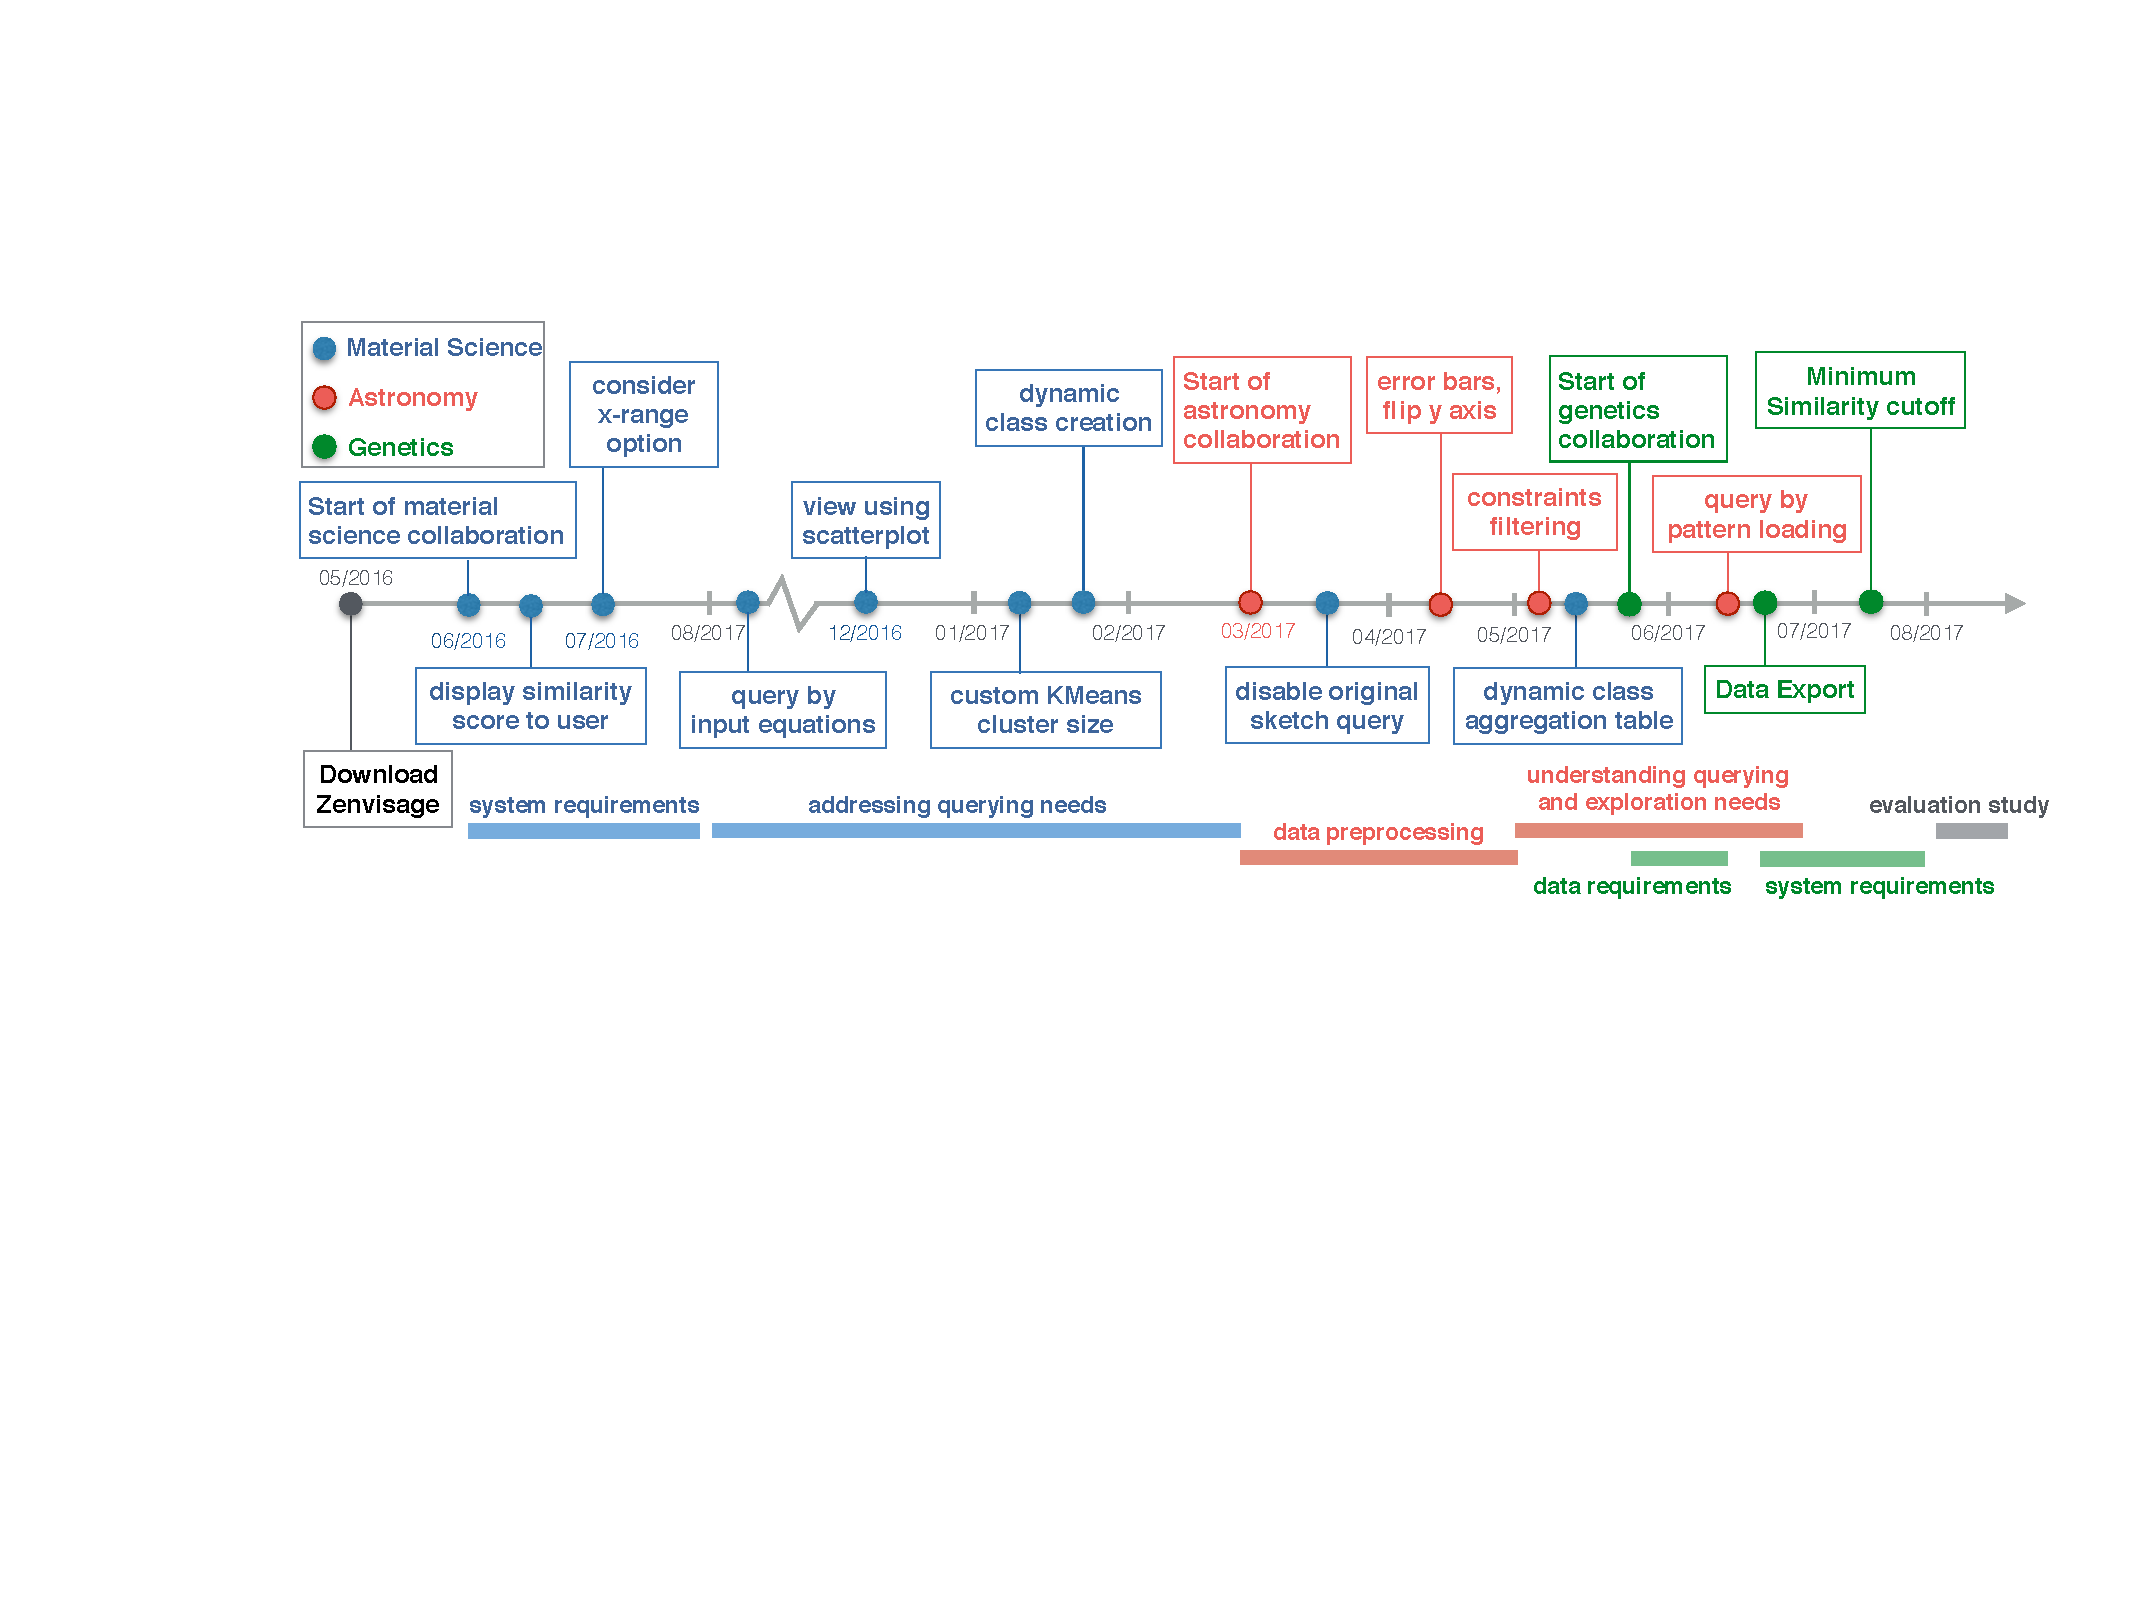
\includegraphics[width=6in]{figures/timeline_anon.pdf}
	\vspace{-6pt}\caption{Timeline for progress in participatory design studies.}
	\label{timeline}
	\vspace{-10pt}
\end{figure*}
\par Via cognitive walkthroughs and interviews, we first identified challenges in existing data analysis workflows in these domains
that could be potentially addressed by a VQS. Building on top of an existing, open-source VQS, \zv~\cite{Siddiqui2017,Siddiqui2017VLDB}, we collaborated closely with our participants to gather feedback and iterate on VQS feature designs,
over the course of a year, culminating in a new enhanced VQS, \zvpp. We organized these features into a taxonomy of VQS functionalities, involving three sensemaking processes inspired by Pirolli and Card's notional model of analyst sensemaking~\cite{Pirolli}. The sensemaking processes include top-down pattern specification (translating a pattern ``in-the-head'' into the form of a visual query), bottom-up data-driven inquiries (querying or recommending based on data), and context-creation (navigating across different collections of visualizations). We find that prior VQSs have focused largely on top-down processes, while largely ignoring the other two processes that are crucial for the needs in all three domains.
\par To study how various VQS features
are used in practice,
we conducted a final evaluation study with nine participants
using our final VQS prototype, \zvpp,
to address their research questions
on their own datasets.
In a 1.5-hour user study, participants were able to
gain novel scientific insights,
such as identifying a star with a transient pattern
that was known to harbor a Jupiter-sized planet
and finding characteristic gene expression profiles confirming the results of a related publication.\techreport{, and discovering that the dip in an astronomical light curve is caused by saturated imaging equipment overlooked by the existing error-detection pipeline.} \techreport{Participants also gain additional insights about their datasets, including debugging mislabeled features and uncovering erroneous data preprocessing procedure applied to a collaborator's dataset.}
%that goes from a pattern in-the-head to a desired visualization

\par By analyzing the evaluation study results, we discovered that sketching a pattern for querying is often ineffective. This is due to the fact that sketching makes the problematic assumptions that users know the pattern that they want to sketch and are able to sketch it precisely. Instead, participants typically opted for other means of pattern specification---one common mechanism was to drag-and-drop a recommended pattern onto the canvas, and then modify it (e.g., by smoothing it out). However, most VQSs do not support these other mechanisms (as we argued earlier, they typically focus only on top-down sensemaking processes, without covering bottom-up and context creation), partially explaining why such systems have not been widely adopted in practice.
\par Further analysis of how participants
transition between different sensemaking processes
during analysis---including the construction of a Markov Model---illustrated
how participants adopt a diverse set of workflows tailored
to their domains. We find that participants often construct analysis workflows focused around a primary sensemaking process, while iteratively interleaving their analysis with the two other processes. This finding points to how all three sensemaking processes, along with seamless transitions between them, are essential for enabling users to effectively use VQSs for data exploration.%For example, participants often center on a main sensemaking process, while interleaving variations with other two processes as they iterate on an analytic task.
\par To the best of our knowledge, our study is the \emph{first to holistically examine how VQSs can be designed to fit the needs of real-world
analysts and how they are actually used in practice}. Our contributions include:
\begin{denselist}
\item a characterization of the problems addressable by VQSs through design studies with three different domains,
\item the construction of a taxonomy of functionalities within VQSs, as well as an articulation of the problem space that is amenable to VQSs, both grounded in participatory design findings,
\item \change{an integrative} VQS, \zvpp, capable of facilitating rapid hypothesis generation and insight discovery,
\item study findings on how VQSs are used in practice, leading to the development of a novel sensemaking model for VQSs. %including the ineffectiveness of
%evaluation
% sketching and the ---- workflow
\end{denselist}
Our work not only opens up a new space of opportunities beyond the narrow use cases considered by prior studies, but also advocates common design guidelines and end-user considerations for building next-generation VQSs.
 %From these experiences, we  advocate visualization researchers and tool designers to ---- future VQS opportunities  Understanding the design space and opportunities for VQS
% Our three main research questions are as follows:

%and not as commonly ---- due to the --- challenges ----. that ----- characteristic workflows ---- iterative sensemaking loop.
%Our collaborative design experience culminated in a full-fledged VQS, \zvpp, described in Section~\ref{sec:pd_findings}.
% \noindent \emph{RQ1: What are the challenges in existing scientific data analysis workflows that could be potentially addressed by a VQS?}
% \par Via cognitive walkthroughs and interviews,
% we gained an understanding of the data analysis
% workflows presently employed by the scientists, their needs,
% and the challenges they face.
% We identified opportunities where a VQS could
% help accelerate their analysis, by helping them
% discover insights, gain intuition, or provoke directions
% for exploration. Finally, we determined the types of
% research questions and dataset properties that would
% be most suitable for exploration on VQSs.
%By learning about the needs and challenges that scientists face when working with their datasets through interviews and cognitive walkthroughs, we learned about the types of queries that they would like to pose on VQSs and distilled a set of design specifications that can better enable VQSs to help them discover insights, gain intuition about their datasets or provoke further directions for exploration. We also identify the types of research questions and dataset properties would be suitable for data exploration on VQSs.
% \begin{figure*}[ht!]
% \centering
% \vspace{-15pt}
% 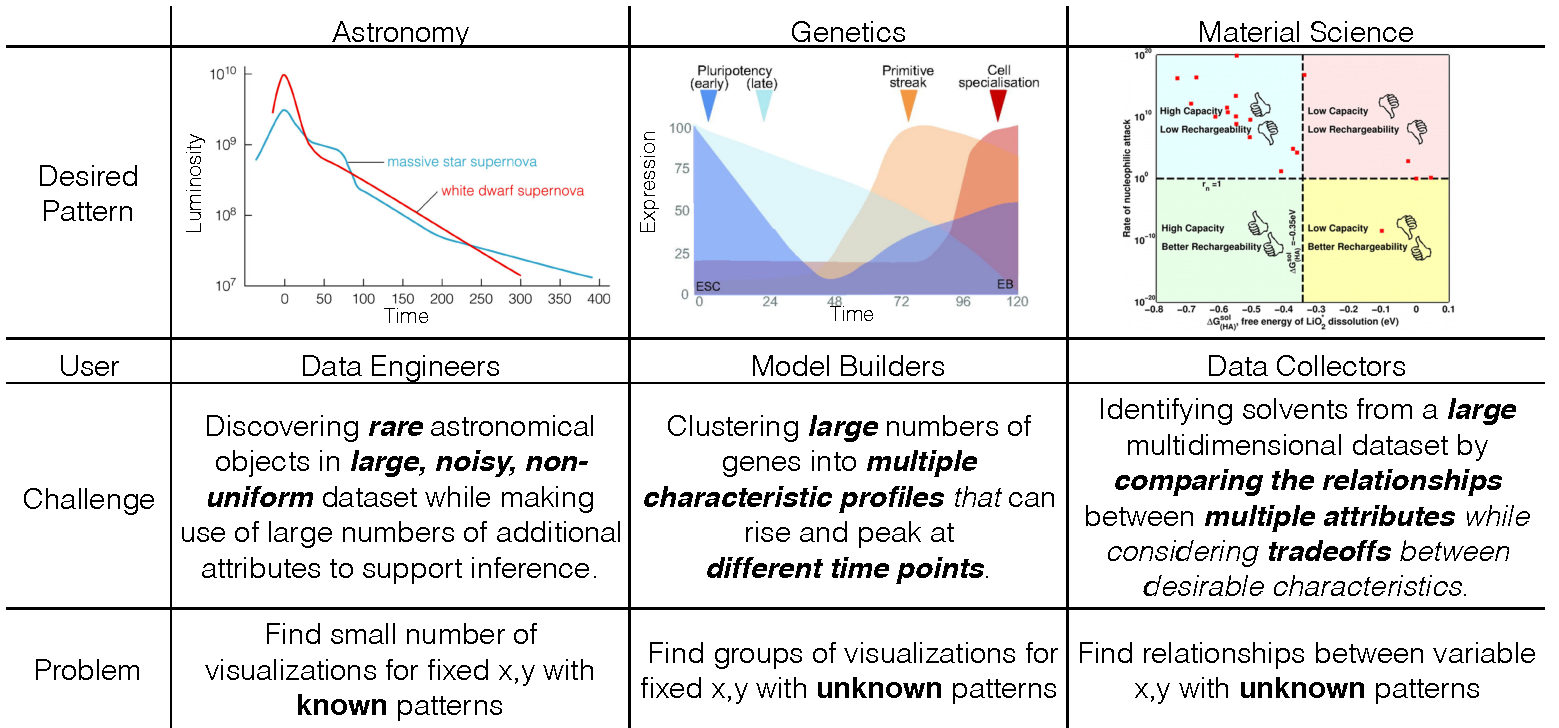
\includegraphics[width=0.8\linewidth]{figures/sci_challenge_tbl.pdf}
% \vspace{-6pt}\caption{Descriptions of the three scientific use cases discussed in this paper.}
% \label{example}
% \vspace{-10pt}
% \end{figure*}

% \noindent \emph{RQ2: What types of interface capabilities are necessary to develop VQSs into a useful component of data analysis?}
% \par Via participatory design, we distilled
% \tvcg{Based on our early interactions with scientists,
% we started to build a VQS~\cite{Siddiqui2017VLDB,Siddiqui2017} that, similar to existing VQSs~\cite{wattenberg2001sketching}, allowed them to search for desired trends via drawing on a canvas. This early system served as a functional prototype for us to engage with scientists further in the participatory design process, understand how they envision themselves using a VQS, and gather feedback on feature designs that could make the VQS more useful. The features we developed address challenges shared across the three scientific domains, ranging from additional querying modalities, to features that support a more integrated workflow, to improving the interpretability of the system output, \tvcg{most of them missing in} prior VQSs in the literature. Our collaborative design experience culminated in a full-fledged VQS, \zv, capable of facilitating rapid hypothesis generation and insight discovery.}

% \noindent \emph{RQ3: How do VQSs accelerate scientific insights?} and \emph{RQ4: How can VQSs fit within the context of existing data analysis workflows?}
% \\ To evaluate our final system \zv, we conducted a user study with nine scientists (including those who had participated in the design process), all of whom had a vested interest in using a VQS to address their research questions on their datasets. In a 1.5-hour user study, our scientist participants were able to gain novel scientific insights, such as \emph{\tvcg{identifying a star with a transient pattern that was known to harbor a Jupiter-sized planet,} finding characteristic gene expression profiles that confirmed the results of a related publication, and learning that the dip in an astronomical light curve is caused by saturated imaging equipment overlooked by the existing error-detection pipeline}.  Participants also gained additional insights about their datasets, including debugging \tvcg{mislabelled features and uncovering the erroneous data preprocessing procedure applied to a collaborator's dataset.}
% that the way data is aggregated across multiple experiments is erroneous on a collaborator's dataset.
% We learned how VQSs could be contextualized within scientific data analysis workflows and discovered that VQSs can be used beyond the exploratory phase of analysis, for data verification, debugging preliminary datasets, and performing sanity-checks on downstream models.

% \begin{figure}[h!]
%     \centering
%     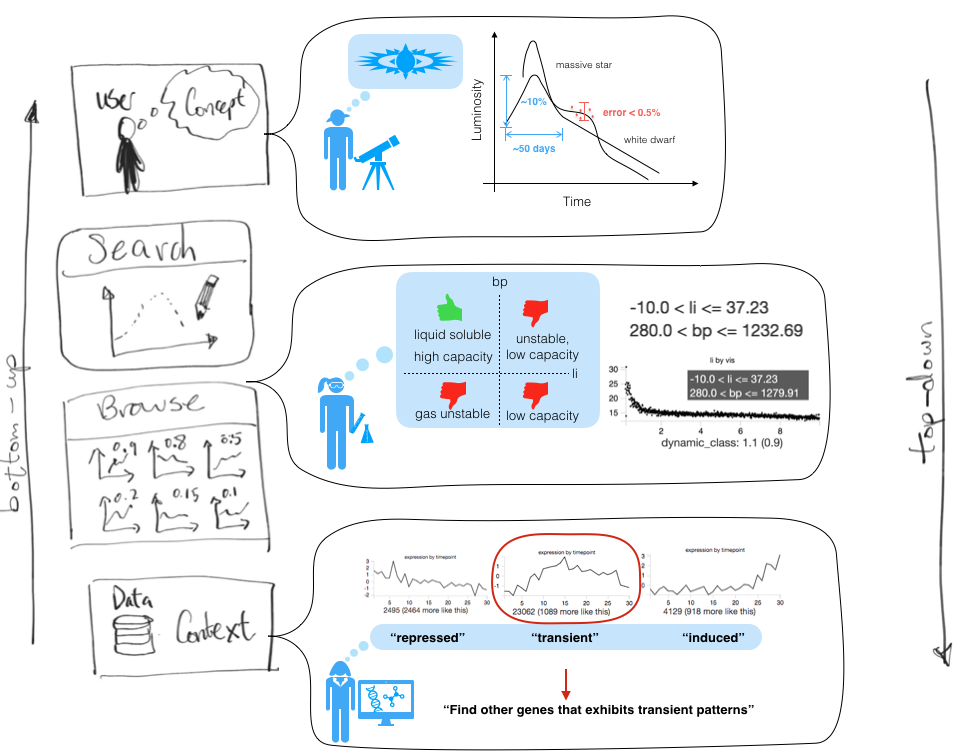
\includegraphics[width=\linewidth]{figures/search-browse-model.png}
%     \vspace{-6pt}\caption{Search Browse Model}
%     \label{fig:sbmodel}
%     \vspace{-5pt}
% \end{figure}

%!TEX root = main.tex
  \section{\change{Related Works\label{sec:relatedworks}}}
  % \subsection{Background and Motivation}
  \par \change{We will now describe past work in visual query systems and existing evaluation methods of visualization systems to provide background and motivation to our work.
  % Visual query systems enable users to directly search for visualizations matching certain patterns through an intuitive specification interface. Early work in this space focused on interfaces to search for time series with specific patterns.
  \par \emph{Visual query systems} (VQSs) is a term coined by Ryall et al. and Correll and Gleicher\cite{ryall2005querylines,correll2016semantics} to describe systems that enable analysts to directly search for time-series visualizations matching certain patterns through an intuitive specification interface. Examples of such systems} include TimeSearcher~\cite{Hochheiser2001,Hochheiser2004}, where the query specification mechanism is a rectangular box, with the tool filtering out all of the time series that does not pass through it, QuerySketch~\cite{wattenberg2001sketching} and Google Correlate~\cite{mohebbi2011google}, where the query is sketched as a pattern on canvas, with the tool filtering out all of the time series that have a different shape. Subsequent work recognized the ambiguity in sketching by studying how humans rank the similarity in patterns~\cite{Eichmann2015,correll2016semantics,Mannino2018} and improving the expressiveness of sketched queries through finer-grained specification interfaces and pattern-matching algorithms~\cite{ryall2005querylines,Holz2009}.
  %performed crowdsourced perceptual studies to understand how humans rank similarity in patterns subjectively
  % , including the use of soft constraints~\cite{ryall2005querylines} and implicit relaxed selection techniques~\cite{Holz2009}.
  % In addition to this ongoing work, recent work have also performed crowdsourced perceptual studies to understand how humans rank similarity in patterns subjectively~\cite{Eichmann2015,correll2016semantics,Mannino2018}.
  \par While these systems have been effective in controlled lab studies, they have never been designed and evaluated in-situ on multiple real-world use cases. Even when use cases were involved~\cite{Hochheiser2004,correll2016semantics}, the inclusion of these \change{case studies served as a post-hoc demonstrative case study that had} little influence on the major design decisions of the system. In the context of Munzner's nested model~\cite{munzner2009nested}, this \change{gap between research and adoption stems from} the common ``downstream threat'' of jumping prematurely into the deep levels of \textit{encoding, interaction, or algorithm design}, before a proper \textit{domain problem characterization} and \textit{data/operation abstraction design} is performed. In this work, we performed design studies~\cite{lam2012empirical,shneiderman2006strategies,Sedlmair2012} with three different subject areas for \textit{domain problem characterization}. Comparing and contrasting between the diverse set of questions, datasets, and challenges across these three use cases revealed new generalizable insights and enabled us to better understand how VQSs can be extended for novel and unforeseen use cases. Based on these findings, we developed a taxonomy for understanding the sensemaking process in VQSs as part of the \textit{data/operation abstraction design}. Finally, we validated the abstraction design with grounded evaluation~\cite{Plaisant2004,Isenberg2008}, where we invited participants to bring in their own datasets and research problems that they have a vested interest in to test our final deployed system. \change{Next, we will outline these two phases of our study, deferring details of the study procedures and protocols to the technical report.}%Next, we will describe these two phases of our study in more detail.
  %had a narrow objective and had 
  \begin{table}[h!]
    \vspace*{-10pt}
     \centering
     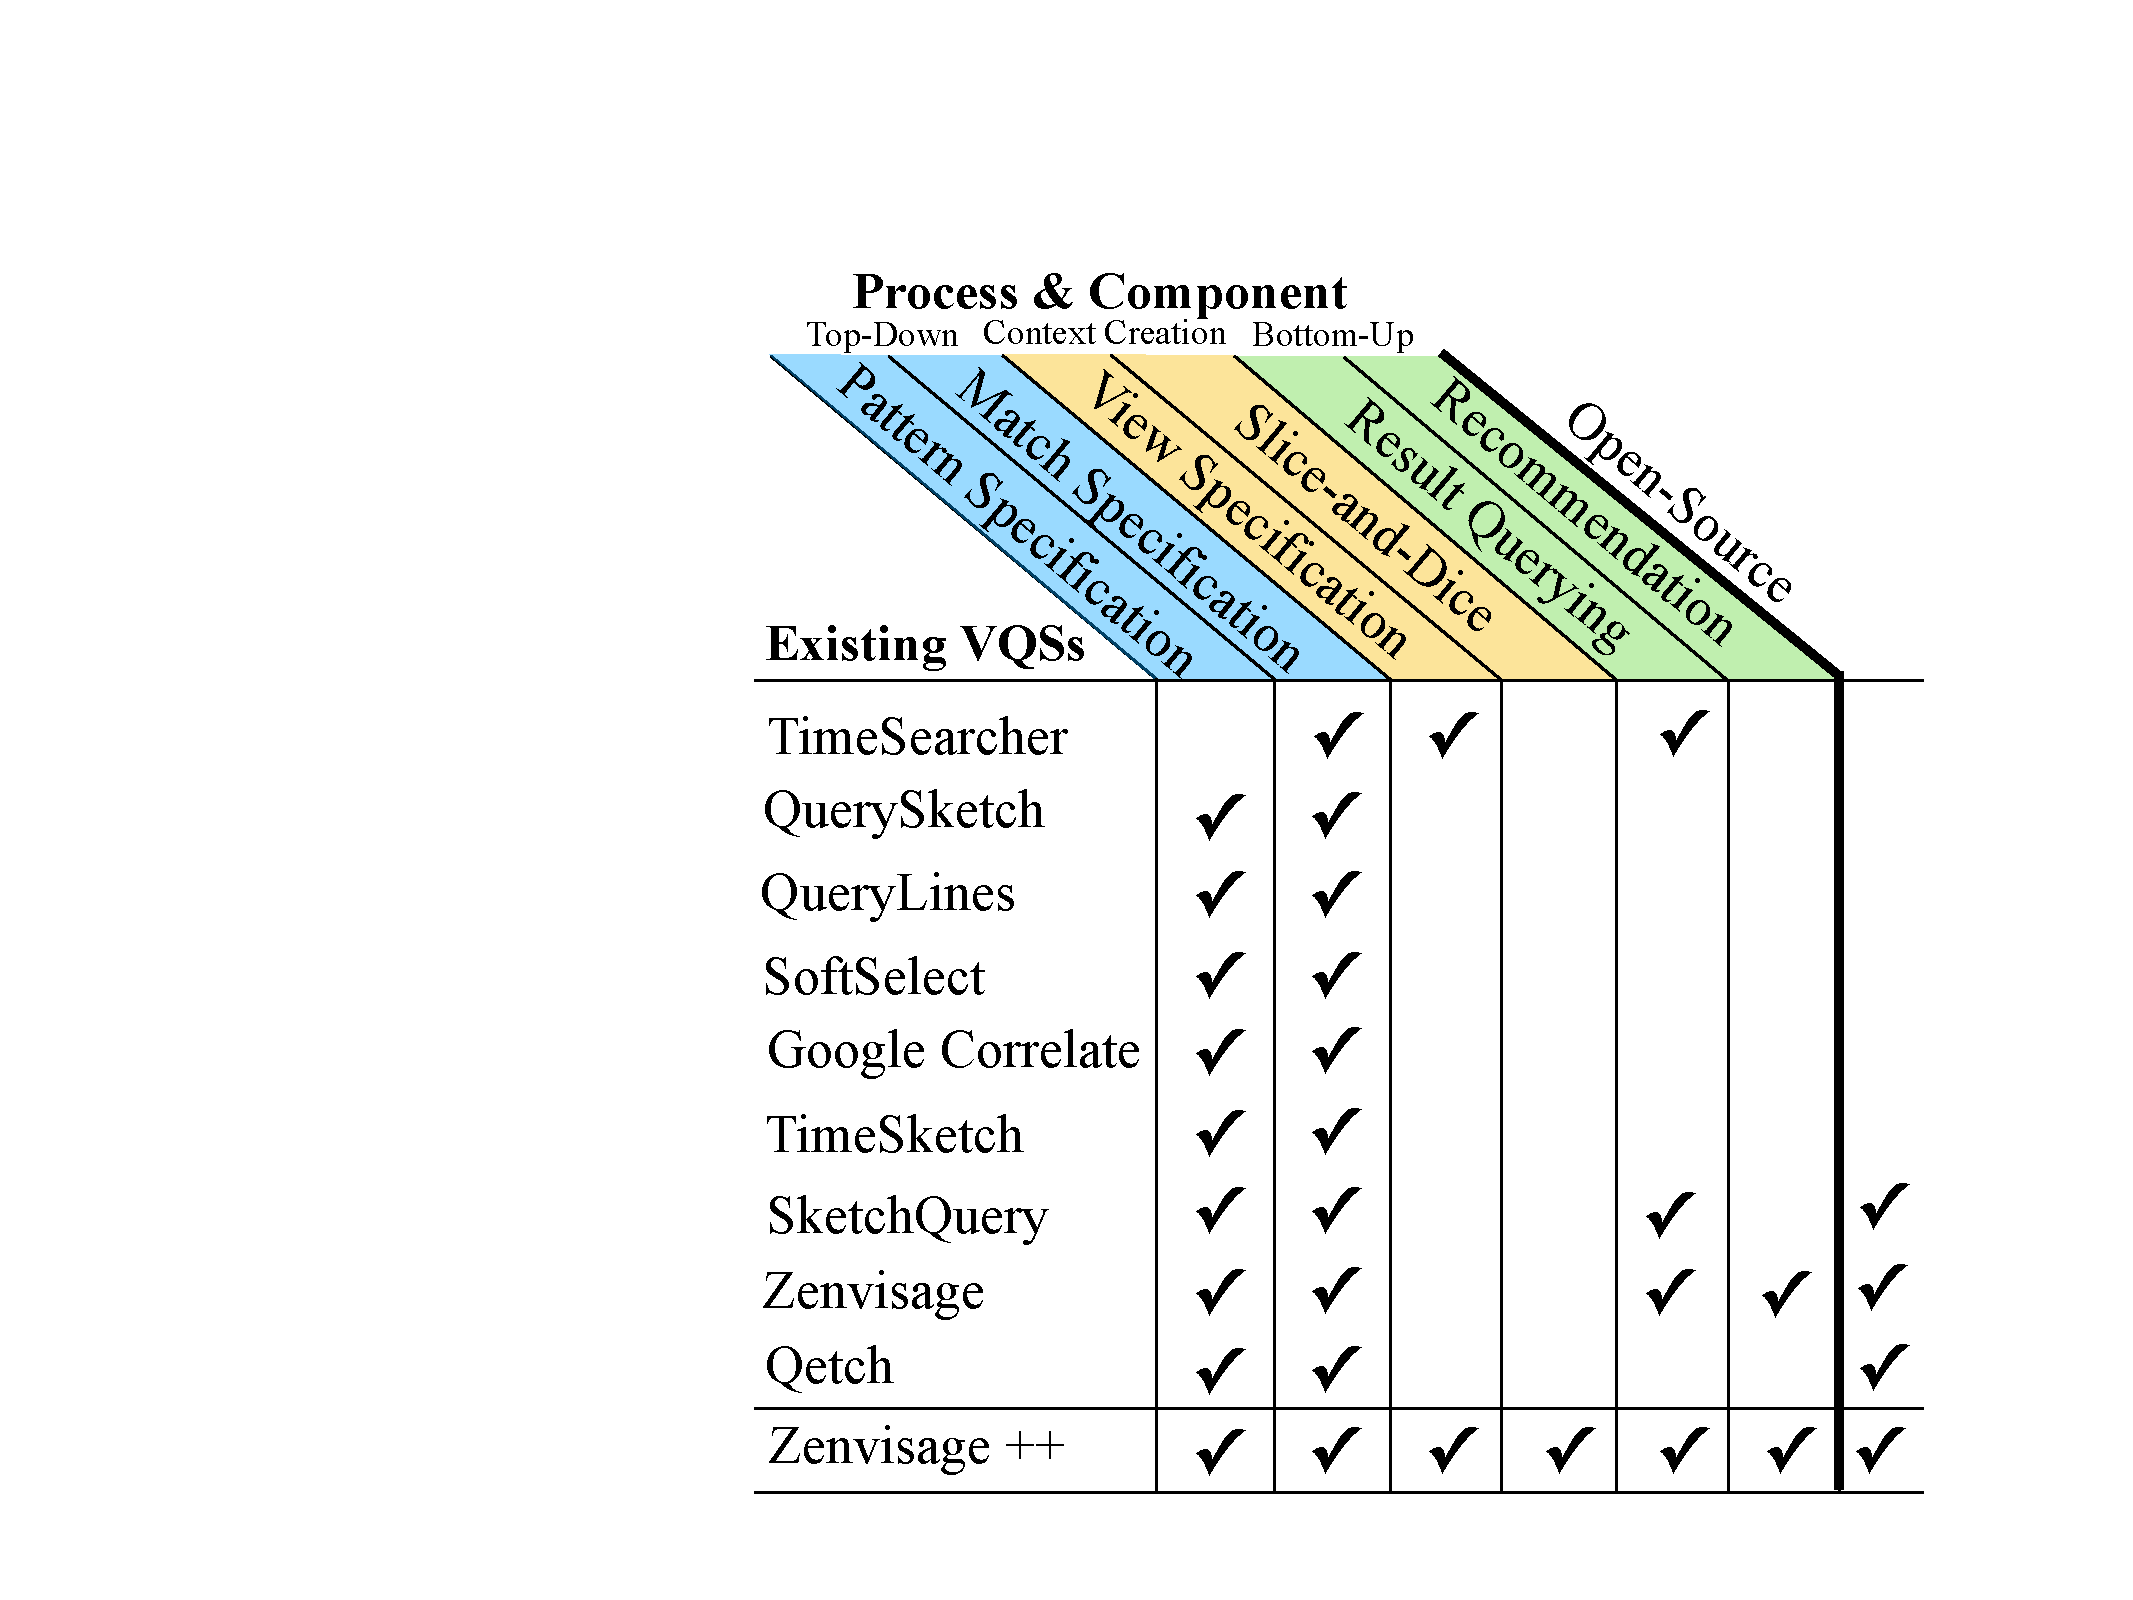
\includegraphics[width=0.8\linewidth]{figures/related_works_table.pdf}
     \caption{Table summarizing whether key functional components (columns) are covered by past systems (row), indicated by checked cells. Column header colors blue, orange, green represents three sensemaking process (top-down querying, search with context, and bottom-up querying) described in Section~\ref{sec:pd_findings}. The heavily-used, practical features in our study for context-creation and bottom-up inquiry is largely missing from prior VQSs.}
     \label{table:relatedwork}
     \vspace*{-15pt}
 \end{table}
%!TEX root = main.tex
\tvcg{\section{Methods} \label{methods}}
%\subsection{Evaluation Methods For Visualization Systems}
\tvcg{\subsection{Methodology Background\label{methodology_relatedwork}}}
\par Visualization systems are often evaluated using controlled studies that measure the user's performance against an existing visualization baseline~\cite{Plaisant2004}. Cognitive measures such as insight time~\cite{North2006,Yi2008} have been developed to capture how well users perform on a task against existing baselines. However, since the operations, hypotheses generated, and insights obtained through exploratory analysis are variable and subjective to individual users and their analytic goals, it is impossible to define tasks beforehand and compare across control groups. Techniques such as artificially inserting ``insights'' or setting predefined tasks for example datasets work well for objective tasks, such as debugging data errors~\cite{kandel2011wrangler,Patel2010}, but this contrived method is unsuitable for trying to learn about the types of real-world queries a user may want to pose on a VQS. \techreport{In order to make the user study more realistic, we opted for a qualitative evaluation where we allowed participants to bring a dataset that they have a vested interest in to address an unanswered research question.}
\par Due to the unrealistic nature of controlled studies, many have proposed using a more multi-faceted, ethnographic approach to understand how analysts perform visual data analysis and reasoning~\cite{Plaisant2004,lam2012empirical,shneiderman2006strategies,munzner2009nested,Sedlmair2012}. For example, multi-dimensional, in-depth, long-term case studies (MILCs) advocate the use of interviews, surveys, logging and other empirical artifacts to create a holistic understanding of how a visualization system is used in its intended environment \cite{shneiderman2006strategies}. Some papers have explored designing visualization and collaborative tools for scientific workflows through individual case studies, e.g.,~\cite{Poon2008,Chen2016}. Similarly, in our work, real-world case studies help us situate how VQSs could be used in the context of an existing analysis workflow.  
\par We adopt {\em participatory design} practices in this work: participatory design ``allows potential users to 
 participate in the design of a system that they will ultimately use''~\cite{Gould1983,Muller1993}. Participatory design has been successfully used in the development of interactive visualization systems in the past~\cite{Aragon2008,Chuang2012}. \tvcg{\cite{Sedlmair2012} highlights the benefits and pitfalls of design study. They advocate that design study methodology is suitable for use cases in which the data is available for prototyping, but the task is only partially known and information is partially in the user's head. In that regard, our scientific use cases with VQS is well-suited for a design research methodology, as we learn about the scientist's data and analysis requirements and design interactions that helps users elicit their ``in-the-head'' specifications into actionable visual queries.} %\cut{In this work, we collaborated with scientists early on to develop features in \zv that address their analysis needs.}  
\tvcg{\subsection{Our Approach}}
\par We adopted a mixed methods research methodology that draws inspiration from ethnographic methods, iterative and participatory design, and controlled studies~\cite{jorgensen_2008,miller_salkind_miller_2002,shneiderman2006strategies,Muller1993} to understand how VQSs can accelerate scientific data analysis. Our methodology served to address the research questions outlined in the introduction. Working with researchers from three different scientific research groups, we identified the needs and challenges of scientific data analysis and the potential opportunities for VQSs to fit in, via interviews and cognitive walkthroughs{\em (RQ1)}. We further extended an existing VQS, \zv, with features for scientists via participatory design{\em (RQ2)}  
\par \tvcg{We chose to build on top of \zv as functional prototype in the design study. The use of functional prototypes is common in participatory design to provide a starting point for the participants. For example, \cite{Ciolfi2016} studied two different alternatives to co-design (starting with open brief versus functional prototype) in the development of museum guidance systems and found that while both approaches were equally fruitful, functional prototypes can make addressing a specific challenge more immediate and focused (in our case the challenge is making comparison across large numbers of visualizations as we found in through informal discussions with practitioners). Our motivation for providing a functional prototype at the beginning of the participatory design sessions is to showcase capabilities of VQSs. Especially since VQSs are not uncommon in the existing workflow of these scientists, participants may not be able to imagine their use cases without a starting point.} %\sout{our prototypical VQS, since it is open-source, has both canvas-based querying capabilities as well as visualization recommendations. (\zv also has a sophisticated query language, ZQL, that we did not employ.)} 
\par As shown in Figure \ref{oldZV}, the basic version of \zv that we built on allowed users to sketch a pattern or drag-and-drop an existing visualization as a query, and \zv would then return visualizations that had the closest Euclidean distance from the queried pattern. The system also displayed representative and outlier patterns to help provide  an overview of typical trends.
	\begin{figure}[ht!]
	\centering
	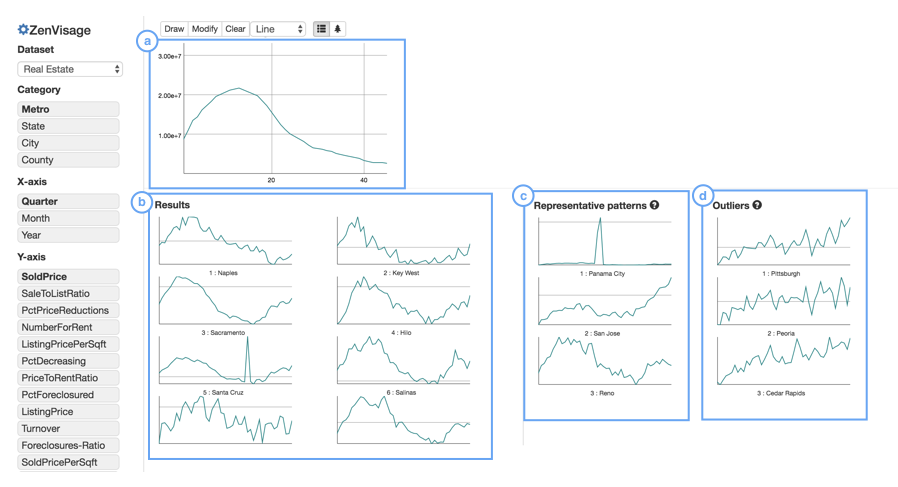
\includegraphics[width=\linewidth]{figures/oldZV_nozql.png}
	\caption{The basic version of \zv that we built on top of allowed users to sketch a pattern in (a), which would then return (b) results that had the closest Euclidean distance from the sketched pattern. The system also displays (c) representative patterns obtained through K-means clustering and (d) outlier patterns to help the users gain an overview of the dataset. \tvcg{The details of the system is described in our previous work \cite{Siddiqui2017,Siddiqui2017VLDB}.}}
	\label{oldZV}
	\end{figure}
\par After incorporating desired features into \ourVQS over the period of a year, we conducted a qualitative evaluation to study how our improved VQS affected the way the users explore their data{\em (RQ3,4)} . \cut{It is interesting to note that not all of the features suggested by the participants were found to be useful during our evaluation.}
\begin{table}[h]
\centering
\vspace{-10pt}
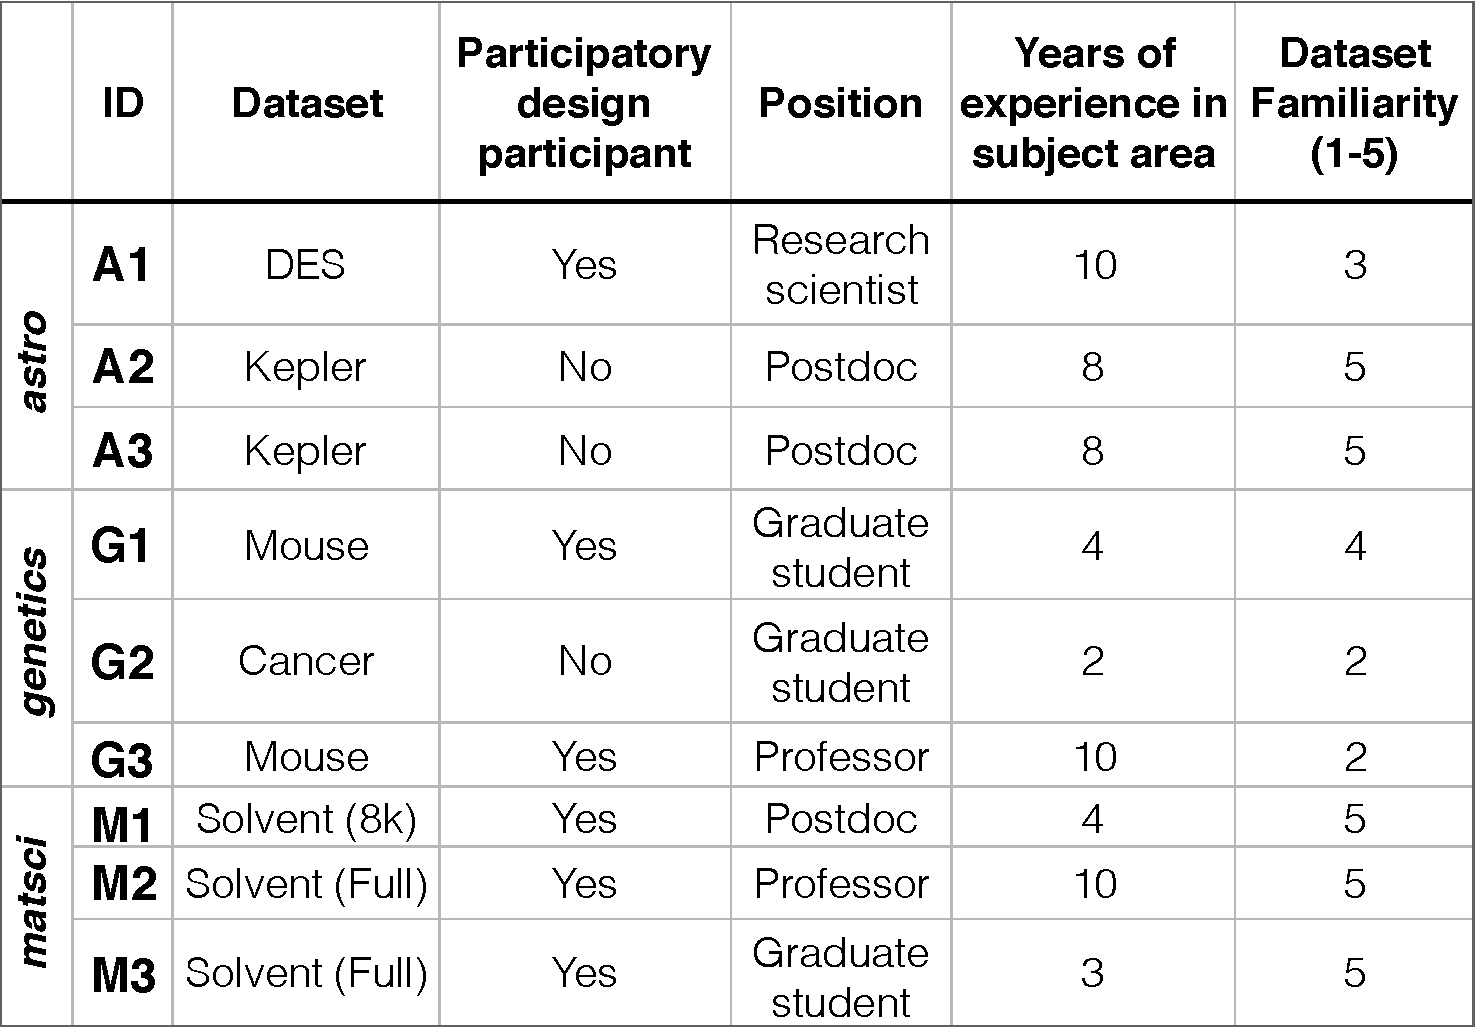
\includegraphics[width=\linewidth]{figures/participants.pdf}
\caption{Participant information. The Likert scale used for dataset familiarity ranges from 1 (not at all familiar) to 5 (extremely familiar).}
\label{participants}
\vspace{-10pt}
\end{table}
\tvcg{\section{Understanding Scientific Data Analysis (R1)}}
%\cut{ \subsection{Understanding Scientific Data Analysis}
%\par Our initial inspiration for building a VQS came from informal discussions with many academic and industry analysts. Their current workflows required the analysts to manually examine a large number of visualizations to derive insights from their data. In this section, we address RQ1 by understanding the limitations and opportunities in existing scientific data analysis workflows in three research areas. We begin by describing the participants in these areas.} 
\subsection{Participants, Datasets and Workflows}
We recruited participants by reaching out to research groups who were interested in using VQSs for exploring their data via email.\dor{Not sure if we should make this more general about challenges in data analysis rather than focus on VQS to correspond to our earlier statement.} We summarize the common properties and differences of these three groups of researchers in Figure~\ref{example} and the desirable characteristics common to these datasets suitable for VQSs in \tvcg{the Section~\ref{metastudy}}. Six scientists from three research groups participated in the design of \zv. The evaluation study participants included these six scientists, along with three ``blank-slate'' participants who had never encountered \zv before. While participatory design subjects actively provided feedback on \zv with their data, they only saw us demonstrating their requested features and explaining the system to them, rather than actively using the system on their own. So the evaluation study was the first time that all nine of the participants used \zv to explore their datasets. We list the participants in Table~\ref{participants}, and refer to them by their anonymized ID as listed in the table. 
\techreport{On average, the participants had more than 8 years of experience working in their respective fields.}
\begin{figure*}[ht!]
\centering
\vspace{-10pt}
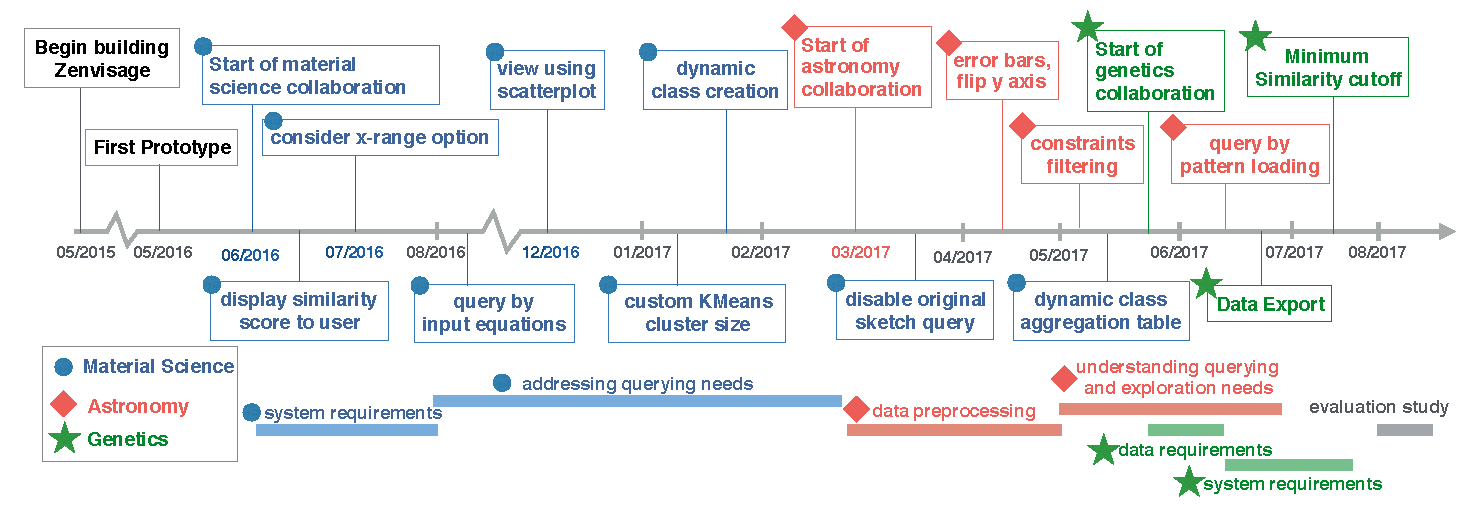
\includegraphics[width=6in]{figures/timeline_new.pdf}
\vspace{-6pt}\caption{Participatory design timeline for the scientific use cases.}
\label{timeline}
\vspace{-10pt}
\end{figure*}

\techreport{The research questions and objectives of the participants were diverse even among those in the same subject area and using the same dataset. Examples of research questions included: 
\begin{denselist}
\item Understanding the gene expression profiles of breast cancer cells that exhibit induced, transient, and  repressed patterns after a particular treatment.
\item Studying common patterns among stars that exhibit planetary transits versus stars that don't from the Kepler space telescope\footnote{\url{www.nasa.gov/mission_pages/kepler/main/index.html}}.
\item Identifying battery solvents with favorable properties and mass production potential through studying how changes in certain chemical properties correlate to changes in other chemical properties. \end{denselist}
}
\par The pre-study survey with the participants showed that out of all of the steps in their data analysis workflow\footnote{This includes viewing and browsing data, data cleaning and wrangling, computing statistics, data visualization, and model building or machine learning.}, they spend the most time computing statistics and creating visualizations.
The main bottlenecks cited in their existing workflow included the challenge of dealing with large amounts of data, writing custom processing and analysis scripts, and long turnaround times incurred by making modifications to an upstream operation in a segmented workflow. \ccut{On average, participants expressed interest in adopting \zv in their day-to-day workflow as eight from a Likert scale of ten after the study \kk{not sure what this means}.}
\par During the participatory design process, we collaborated with each of the teams closely with an average of two meetings per month, where we learned about their datasets, objectives, and how VQSs could help address their research questions. A detailed timeline of our engagement with the participants and the features inspired by their use cases can be found in Figure \ref{timeline}. Participants provided datasets they were exploring from their domain, whereby they had a vested interest to use a VQS to address their own research questions. We  describe the three scientific use cases below.

\par \textbf{Astronomy (\astro):} The Dark Energy Survey (DES) is a multi-institutional project with over 400 scientists. Scientists use a multi-band telescope that takes images of 300 million galaxies over 525 nights to study dark energy\cite{Drlica-Wagner2017}. The telescope also focuses on smaller patches of the sky on a weekly interval to discover astrophysical transients (objects whose brightness changes dramatically as a function of time), such as supernova explosions or quasars. The output is a time series of brightness observations associated with each object extracted from the images observed. %\kk{is it 4 years of 525 nights?}\dor{it's a bit confusing, because they only observe half a year on the southern hemisphere, will skip talking about this} 

For over five months, we worked closely with an astronomer on the project's data management team working at a supercomputing facility. \cut{We also gathered feedback from other astronomers who were interested in studying the properties of astrophysical transients during a collaboration-wide meeting.} The scientific goal is to identify a smaller set of potential candidates that may be astrophysical transients in order to study their properties in more detail. These insights can help further constrain physical models regarding the formation of these objects.
\par \textbf{Genetics (\bio):} Gene expression is a common data type used in genomics and is obtained via microarray experiments. \techreport{In these experiments, a grid containing thousands of DNA fragments are exposed to stimuli and measurements for the level at which a gene is expressed are recorded as a function of time.} The data used in the participatory design sessions was the gene expression data over time for mouse stem cells aggregated over multiple experiments, downloaded from an online database\footnote{\url{ncbi.nlm.nih.gov/geo/}}. 
\par  We worked with \tvcg{a graduate student and a PI} at a research university over three months who were using gene expression data to better understand how genes are related to phenotypes expressed during early development~\cite{Peng2016,Gloss084442}. They were interested in using \zv to cluster gene expression data before conducting analysis with a downstream machine learning workflow. 
\par \textbf{Material Science (\matsci):} We collaborated with material scientists at a research university who are working to identify solvents that can improve battery performance and stability. These scientists work with large datasets containing over 25 chemical properties for more than 280K different solvents obtained from simulations. \techreport{Once they have identified a solvent that also produces favorable results in an experiment, they identify other solvents with similar properties,  which may be cheaper or safer to manufacture at an industrial scale.}
\par We worked closely with two graduate students and a PI for over a year to design a sensible way of exploring their data using VQSs\footnote{Note that while we have interacted with the \matsci participant during the initial development stage, the participatory design formally started in June 2016}. Each row of their dataset represents a unique solvent, and consists of 25 different chemical attributes. They wanted to use \zv to identify solvents which have similar properties to known solvents but are more favorable (e.g. cheaper or safer to manufacture), and identify how changes in certain chemical attributes affects them.
\raggedbottom

%%%%%%%%%%%%%%%%%%%%%%%%%%%%%%%%%
\subsection{Cognitive Walkthrough Sessions}
Cognitive walkthroughs highlight the existing workflows and behavior that participants have adopted for conducting certain tasks~\cite{Nielsen1994}. In our case, we observed the participants as they conducted a cognitive walkthrough demonstrating every component of their current data analysis workflow.
\techreport{
	\begin{figure}[ht!]
		\centering
		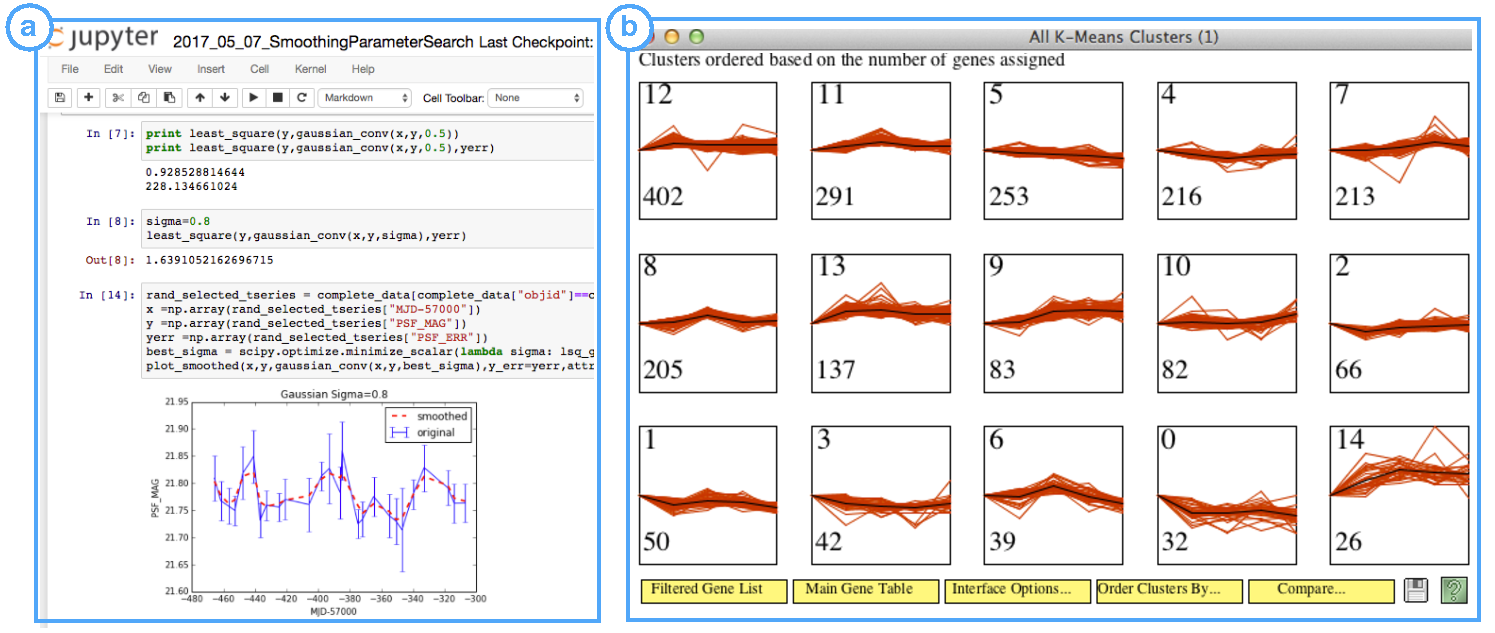
\includegraphics[width=\linewidth]{figures/workflow.pdf}
		\caption{Examples of the scientists' original workflow: a) The astronomer performs various data analysis task using the Jupyter notebook environment, b) The geneticists uses a domain-specific software to examine clustering outputs.}
		\label{workflow}
	\end{figure}
}
\par \textbf{Astronomy:} Since astronomical datasets are often terabytes in scale, they are often processed and stored in highly specialized data management centers in supercomputing centers. The collaboration's data management team has created a command-line interface that enables users to easily query, browse, and download their data\techreport{\footnote{ \url{github.com/mgckind/easyaccess}}}. 
After the data is downloaded, most of the work is done programmatically through Python in an interactive Jupyter notebook environment\footnote{\url{jupyter.org}}. The astronomer inspects the data schema, performs data cleaning and  wrangling, computes relevant statistics, and generates visualizations to search for anomalies or objects of interest, as shown in Figure \ref{workflow}a.
\par While an experienced astronomer who has examined many transient light curves can often distinguish an interesting transient object from noise by sight, they must visually examine and iterate through large numbers of visualizations of candidate objects. Manual searching is time-consuming and error prone as the majority of the objects will not be astronomical transients.
Participant A1 was interested in \zv as he recognized how specific pattern queries could help scientists directly search for these rare objects. 
\techreport{\par If an object of interest or region is identified through the visual analysis, then the astronomer may be interested in inspecting the image of the region for cross-checking that the significant change in brightness of the object is not due to an imaging artifact. This could be done using a custom built web-interface that facilitates the access of cutout images for a queried region of the sky.} 

\par \textbf{Genetics:} Participant G1 processes the raw microarray data by using a preprocessing script written in R \techreport{, where they (i) sub-select 144 genes of interest, (ii) clean up an experimental artifact due to measurements on multiple probes, (iii) log-transform the raw data to show a more distinct shape profile for clustering, (iv) normalize the gene expression values into the range of 0 to 1, and (v) perform Loess smoothing with default parameters to reduce the noise in the data}. To analyze the data, the preprocessed data is loaded into a desktop application for visualizing and clustering gene expression data\footnote{ \url{www.cs.cmu.edu/~jernst/stem/}}. G1 sets several clustering and visualization parameters on the interface before pressing a button to execute the clustering algorithm. The cluster visualizations are then displayed as overlaid time series for each cluster, as shown in the visualization in Figure \ref{workflow}b. G1 visually inspects that all the patterns in each cluster look ``clean'' and checks the number of outlier genes that do not fall into any of the clusters.  If the number of outliers is high or the visualizations look unclean, they rerun the clustering by increasing the number of clusters. Once the visualized clusters look ``good enough'', G1 exports the cluster patterns into a csv file to be used as features in their downstream regression tasks.
\par Prior to the study, the student (G1) and PI (G3) spent over a month attempting to determine the best number of clusters for their upstream analysis based on a series of static visualizations and statistics computed after clustering. While regenerating their results took no more than 15 minutes every time they made a change, the multi-step, segmented workflow meant that all changes had to be done offline, so that valuable meeting time was not wasted trying to regenerate results. The team had a vested interest in participating in the design of \zv as they saw how the interactive nature of VQSs and the ability to query other time series with clustering results could dramatically speed up their collaborative analysis process. 
\par \textbf{Material Science:} Participant M1 starts his data exploration process with a list of known and proven solvents as a reference. For instance, he would search for solvents which have boiling point over 300 Kelvins and the lithium solvation energy under 10 kcal/mol using basic SQL queries. This would help him narrow down the list of solvents, and he would continue this process with other properties. The scientist also considers the availability and the cost of the solvents while exploring the dataset. When the remaining list of the solvents is sufficiently small, he drills down to more detail (e.g., such as looking at the chemical structure of the solvents to consider the feasibility of conducting experiments with the solvent). While he had identified potential solvents through  manual lookup and comparison,  the process lacked the ability to reveal complicated trends and patterns that might be hidden, such as how the change in one attribute can affect the behavior of other attributes of a solvent. M1 was interested in using a VQS as it was infeasible for him to manually compare between large numbers of solvents and their associated properties manually.
\raggedbottom
%!TEX root = main.tex
\section{Participants and Datasets}
During the design study, we observed participants as they conducted a cognitive walkthrough demonstrating their existing data analysis workflow. In this section, we describe our study participants and their use cases to highlight behaviors that participants have adopted for conducting certain analysis tasks.
\par\noindent\stitle{Astronomy:} The Dark Energy Survey (DES) is a multi-institutional project that surveys 300 million galaxies over 525 nights to study dark energy\cite{Drlica-Wagner2017}. The telescope also focuses on smaller patches of the sky on a weekly interval to discover astrophysical transients (objects whose brightness changes dramatically as a function of time), such as supernova explosions or quasars. The output is a time series of brightness observations associated with each object extracted from the images observed. For over five months, we worked closely with an astronomer on the project's data management team working at a supercomputing facility (A1). The scientific goal is to identify a smaller set of potential candidates that may be astrophysical transients in order to study their properties in more detail. \techreport{These insights can help further constrain physical models regarding the formation of these objects.}
\par A1 was interested in \zv as he recognized how specific pattern queries could help scientists directly search for these rare objects. While an experienced astronomer who has examined many transient light curves can often distinguish an interesting transient object from noise by sight, they must visually examine and iterate through large numbers of visualizations of candidate objects. Manual searching is time-consuming and error prone as the large majority of the objects are not astronomical transients.
\techreport{\par If an object of interest or region is identified through the visual analysis, then the astronomer may be interested in inspecting the image of the region for cross-checking that the significant change in brightness of the object is not due to an imaging artifact. This could be done using a custom built web-interface that facilitates the access of cutout images for a queried region of the sky.}
\par\noindent\stitle{Genetics:} Gene expression is a common data type used in genomics and is obtained via microarray experiments. \techreport{In these experiments, a grid containing thousands of DNA fragments are exposed to stimuli and measurements for the level at which a gene is expressed are recorded as a function of time.} The data used in the participatory design sessions was the gene expression data over time for mouse stem cells aggregated over multiple experiments.\techreport{, downloaded from an online database\footnote{\url{ncbi.nlm.nih.gov/geo/}}.} We worked with a graduate student (G1) and professor (G3) at a research university who were using gene expression data to better understand how genes are related to phenotypes expressed during early development~\cite{Peng2016,Gloss2017}. They were interested in using \zv to cluster gene expression data before conducting analysis with a downstream machine learning workflow.
\par To analyze the data, participant G1 loads the preprocessed data into a desktop application for visualizing and clustering gene expression data\techreport{\footnote{\url{www.cs.cmu.edu/~jernst/stem/}}}. Then she sets several clustering and visualization parameters before executing the clustering algorithm, then overlaid time series for each cluster is displayed on the interface. G1 visually inspects that all the patterns in each cluster looks ``clean'' and checks that the number of outlier genes that do not fall into any of the clusters is low.  If the number of outliers is high or the visualizations look unclean, she reruns the analysis by increasing the number of clusters. When the visualized clusters look ``good enough'', G1 exports the cluster patterns into a csv file to be used as features in their downstream regression tasks.
\par Prior to the study, G1 and G3 spent over a month attempting to determine the best number of clusters for their upstream analysis based on a series of static visualizations and statistics computed after clustering. While regenerating their results took no more than 15 minutes every time they made a change, the multi-step, segmented workflow meant that all changes had to be done offline, so that valuable meeting time was not wasted trying to regenerate results. The team had a vested interest in participating in the design of \zv as they saw how the interactive nature of VQSs and the ability to query other time series with clustering results could dramatically speed up their collaborative analysis process.
\par\noindent\stitle{Material Science:} We collaborated with material scientists at a research university who are working to identify solvents that can improve battery performance and stability. These scientists work with large datasets containing over 25 chemical properties for more than 280,000 different solvents obtained from simulations. We worked closely with a a postdoctoral researcher (M1), professor (M2), and graduate student (M3) for over a year to design a sensible way of exploring their data using VQSs. Each row of their dataset represents a unique solvent, and consists of 25 different chemical attributes. They wanted to use \zv to identify solvents that not only have similar properties to known solvents but also are more favorable (e.g. cheaper or safer to manufacture), as well as to understand how changes in certain chemical attributes affects them.
\par Participant M1 starts his data exploration process by iteratively applying filters on a list of potential battery solvents using SQL queries. When the remaining list of the solvents is sufficiently small, he examines each solvent in more detail to weigh in the cost and availability to determine experimental feasibility. Participant M1 was interested in using a VQS as it was impossible for him to uncover hidden relationships (such as how changing one attribute affects another attribute) between large number of solvents manually.
\dor{Need to emphasize how known/unknown pattern and attribute for each usage case}
%!TEX root = main.tex
 %\section{System-level Participatory Design Findings\label{sec:pd_findings}}
 \section{Design Process and System Overview\label{sec:pd_findings}}
%All of the three domains described in the previous section recognized the need for a VQS. As discussed in Section~\ref{sec:methods},
%we worked closely with participants to develop features to address their problems and challenges.
 Given the need for a VQS highlighted via contextual inquiries, we further collaborated with participants to develop features to address their problems and challenges. In this section, we first reflect on our feature discovery process to introduce our \rchange{design findings}, then we provide a high-level system overview of the \rchange{design} product, \zvpp.
 \subsection{The Collaborative Feature Discovery Process~\label{sec:feature_dsicovery}}
 \par Throughout the \rchange{design} process, we worked closely with participants to discover VQS capabilities that were essential for addressing their high-level domain challenges. We identified various subtasks based on the participant's workflow, designed sensible features for accomplishing these subtasks that could be used in conjunction with existing VQS capabilities, and elicited feedback on intermediate feature prototypes. Bodker et al.~\cite{BodkerGronbaek} cite the importance of encouraging user participation and creativity in cooperative design through different techniques, such as future workshops, critiques, and situational role-playing. Similarly, our \cut{PD} objective was to collect as many feature proposals as possible, while being inclusive across different domains. We further organized these features into Table~\ref{bigfeaturetable} through an iterative coding process by one of the authors.
 \par In grounded theory methods~\cite{Muller2012}, researchers first create \emph{open codes} to assign descriptive labels to raw data, followed by grouping open codes together by relationships or categories to form \emph{axial codes}. Finally, \emph{selective codes} are obtained by focusing on specific sets of axial codes to come up with a set of core emerging concepts. Inspired by grounded theory methods, we first collected the list of features and example usage scenarios \cut{from PD} and similar capabilities in existing VQSs as open codes. Then, we further organized this list into axial codes representing ``components'' (first column in Table~\ref{bigfeaturetable}): core functionalities that are essential in VQSs. Finally, as we will describe in Section~\ref{sec:sensemaking}, the selective codes capture each of the sensemaking processes (denoted by cell colors in Table~\ref{bigfeaturetable}). Instead of describing this table in detail, we present a typical example of how this table is organized. Consider row 4 of Table~\ref{bigfeaturetable}: one of the common challenges in astronomy and material science is that noise in the dataset can result in large numbers of false-positive matches. To address this issue, smoothing is a feature in \zvpp that enables users to adjust data smoothing algorithms and parameters on-the-fly to both denoise the data and change the degree of shape approximation applied to all visualizations when performing pattern matching. %smoothing is a feature in \zvpp that enables users to adjust data smoothing algorithms and parameters on-the-fly to both denoise the data and change the degree of shape approximation applied to all visualizations when performing pattern matching. This is useful for domains such as astronomy and material science where the dataset is noisy with large numbers of false positives that could be matched to any given pattern query. 
 Smoothing, along with range selection and range invariance (row 5 and 6), is part of the \emph{match specification} component: VQS mechanisms for clarifying how matching should be performed. Both match specification and \emph{pattern specification} (a description of what the pattern query should look like) are essential components for supporting the sensemaking process top-down pattern search (in blue).%, described in Section~\ref{sec:sensemaking}.
 % Smoothing is also supported in Qetch~\cite{Mannino2018}. Other interfaces have also developed constrained sketching mechanisms to allow users to partially specify certain shape characteristics, such as angular slope queries\techreport{for specifying the slope of a trend line}~\cite{Hochheiser2004} or piecewise trend querylines\techreport{over a specified data range}~\cite{ryall2005querylines}. Smoothing was chosen over these other interfaces for approximating key patterns in the data, since it was a familiar preprocessing step in our study participants' workflow.
 \par It is important to note that while some of the proposed features in Table~\ref{bigfeaturetable} (such as data filtering and view specification) are pervasive in general visual analytics (VA) systems~\cite{Heer2012,Amar2005}, they have not been incorporated in present-day VQSs. In fact, one of the key contributions of our work is recognizing the need for an \emph{integrative} VQS whose sum is greater than its parts, that encourages analysts to rapidly generate hypotheses and discover insights by facilitating all three sensemaking processes. This finding is partially enabled by the unexpected benefits that come with collaborating with multiple groups of participants during the feature discovery process, described next.
 \par Given the highly-evolving, ad-hoc nature of exploratory data analysis~\cite{Keim2006,Tukey1970}, our collaborative feature discovery approach for aiding such analysis comes with its advantages and limitations. One such advantage is that introducing the newly-added features to \zvpp that addressed a particular domain often resulted in unexpected use cases for other domains. Considering feature proposals from multiple domains can also lead to more generalized design choices. For example, around the same time when we spoke to astronomers who wanted to eliminate sparse time series from their search results, our material science collaborators also expressed a need for inspecting only solvents with properties above a certain threshold. Through these use cases, data filtering arose as a crucial, common operation that was later incorporated into \zvpp to support this class of queries. %User requests (or lack thereof) may not always translate to a direct need.
 %, leading to a comprehensive list of added features listed in Table~\ref{bigfeaturetable}.
 % \agp{should we have topic sentences to organize takeaways better}
 \begin{figure*}[ht!]
   \centering
   \vspace{-5pt}
   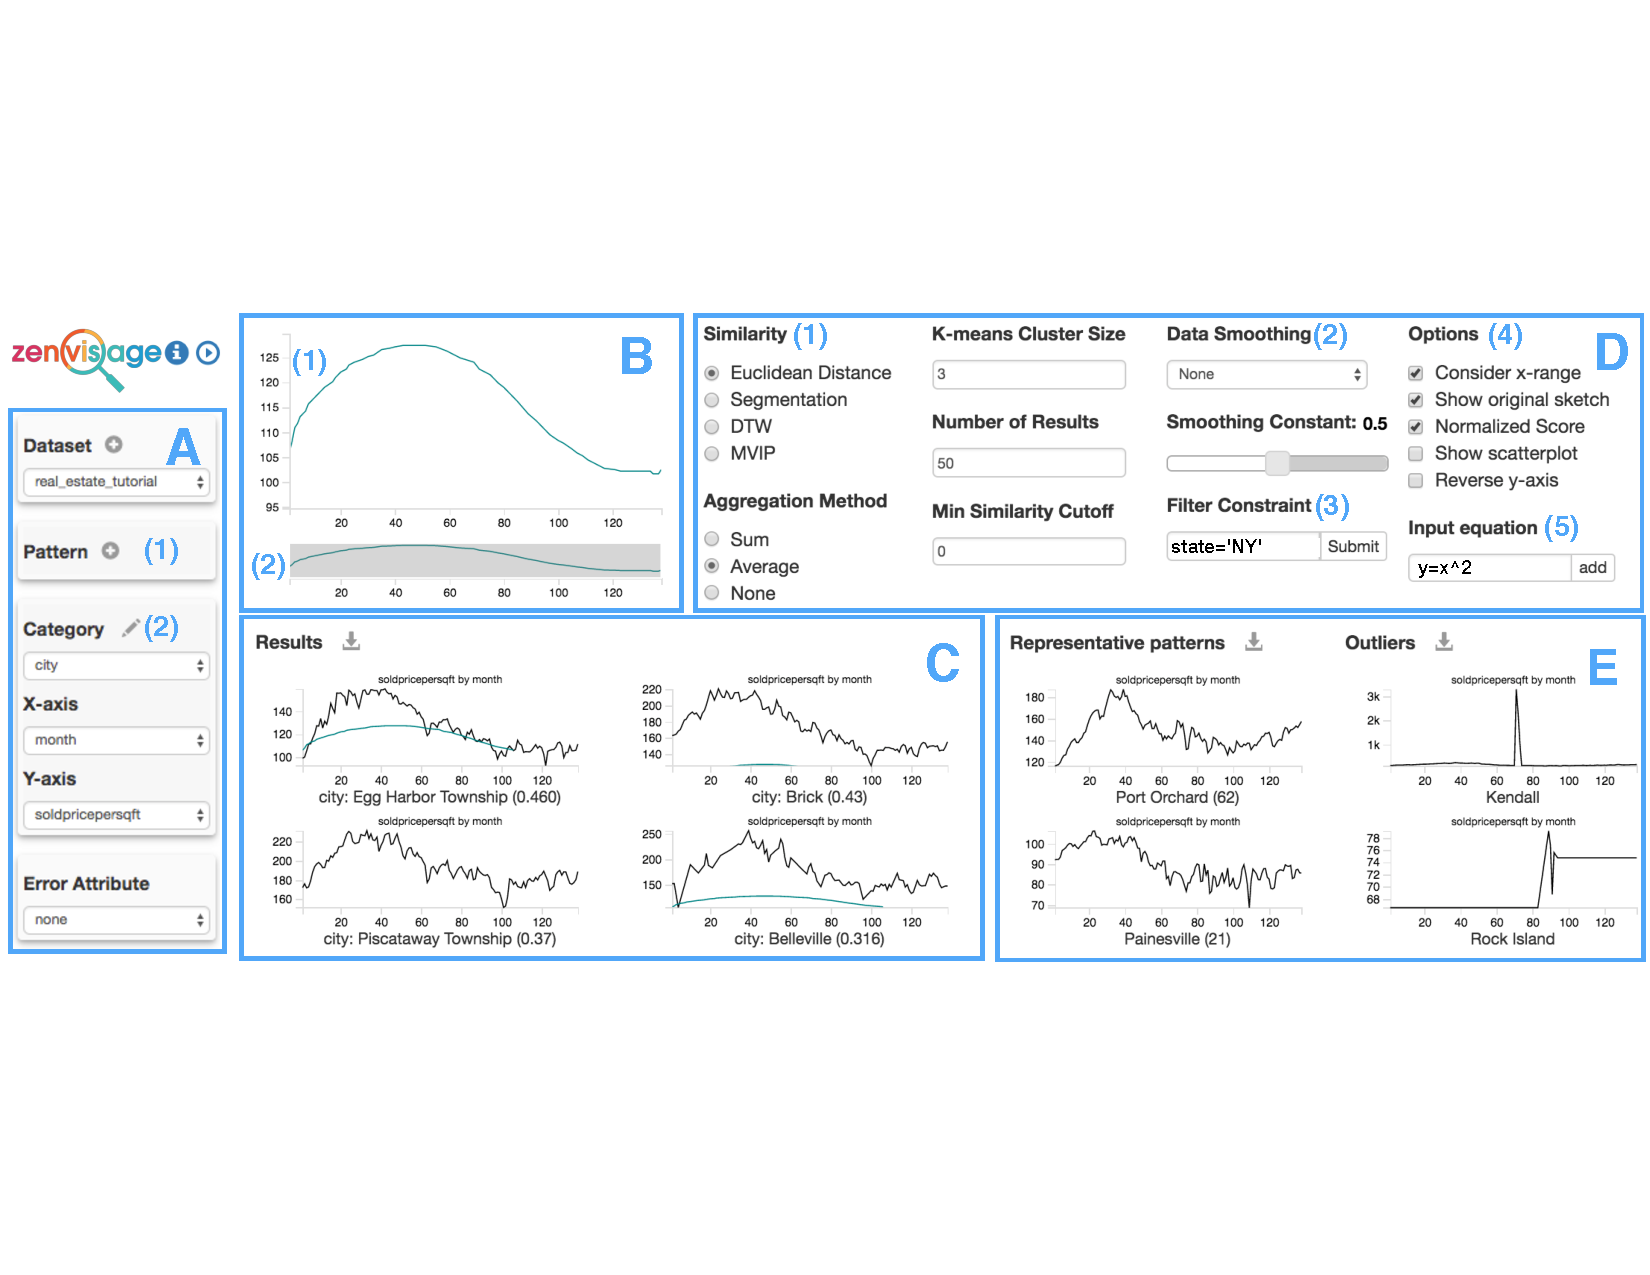
\includegraphics[width=0.9\linewidth]{figures/zvpp_system.pdf} %5.5
   \vspace{-5pt}\caption{The \zvpp system consists of : (A) data selection panel (where users can select visualized dataset and attributes), (B) query canvas (where the queried data pattern is submitted and displayed), (C) results panel (where the visualizations most similar to the queried pattern are displayed as a ranked list), (D) control panel (where users can adjust various system-level settings), and (E) recommendations (where the typical and outlying trends in the dataset is displayed).}
   \label{zvOverview}
   \vspace*{-10pt}
 \end{figure*}
 \par While our collective brainstorming led to the cross-pollination and generalization of features, this technique can also lead to unnecessary features that result in wasted engineering effort. During the design phase, there were numerous problems and associated features proposed by participants, not all of which were incorporated. We detail the list of criteria that was used to determine whether to implement a proposed feature (including eliminating features that were nice-to-have, one-shot operations, non-essential, or required a substantially different set of research questions) in Appendix~\ref{apdx:pdartifact}. Failure to identify these early signs in the design phase may result in feature implementations that turn out not to be useful for the participants or result in feature bloat.
 \subsection{System Overview\label{sec:system}}% as described in the Figure~\ref{timeline} timeline
 The features in Table~\ref{bigfeaturetable} were incrementally incorporated and improved over time, leading to our final \cut{PD product}\rchange{prototype}, \zvpp. Given the space limitations, we will focus our discussion on the major capabilities relevant to the study findings, and defer the details of other features to the appendix and online documentation\footnote{Documentation: \url{http://github.com/zenvisage/zenvisage/wiki}}. The \zvpp interface is organized into 5 major regions all of which dynamically update upon user interactions. Typically, participants begin their analysis by selecting the dataset and attributes to visualize in the \emph{data selection panel} (Figure~\ref{zvOverview}A). Then, they specify a pattern of interest as a query (hereafter referred to as \emph{pattern query}), through either sketching, inputting an equation, uploading a data pattern, or dragging and dropping an existing visualization, displayed on the \emph{query canvas} (Figure~\ref{zvOverview}B). \zvpp performs shape-matching between the queried pattern and other possible visualizations, and returns a ranked list of visualizations that are most similar to the queried pattern, displayed in the \emph{results panel} (Figure~\ref{zvOverview}C). At any point during the analysis, analysts can adjust various system-level settings through the \emph{control panel} (Figure~\ref{zvOverview}D) or browse through the list of \emph{recommendations} provided by \zvpp (Figure~\ref{zvOverview}E). For comparison, the existing \zv system (Figure~\ref{oldZV} in Appendix~\ref{apdx:pdartifact}) from~\cite{Siddiqui2017} allowed users to query via sketching or drag-and-drop and displayed representative and outlier pattern recommendations, but had limited capabilities to navigate across different data subsets and had few control settings. Our \zvpp system is open source and available at: \url{http://github.com/zenvisage/zenvisage}. %\techreport{Our \zvpp system is open source and available at: \url{github.com/[Annonymized for Submission]}.}
 
%!TEX root = main.tex
 \section{A Sensemaking Model for VQSs\label{sec:sensemaking}}
   %To convey how features in \zvpp address the analytical needs posed by each domain, we organize our PD findings into a sensemaking framework for VQSs. As shown in Figure~\ref{fig:taxonomy}, we develop a taxonomy for organizing VQS capabilities into three sensemaking processes.
 Now that we have described our eventual PD prototype \zvpp, we revisit Table~\ref{bigfeaturetable} in an effort to contextualize our PD findings using \change{Pirolli and Card's sensemaking framework~\cite{Pirolli}}. We \change{demonstrate} how features in \zvpp address the analytical needs posed by each domain. We organize the components in Table~\ref{bigfeaturetable} along a taxonomy of three sensemaking processes, as shown in Figure~\ref{fig:taxonomy}. %Our VQS sensemaking model is inspired by Pirolli and Card's information foraging framework~\cite{Pirolli}, which distinguishes between information processing tasks that are \textit{top-down} (from theory to data) and \textit{bottom-up} (from data to theory).
 %\change{The sensemaking model was designed for studying how analysts perform ``intelligence analysis'' (bearing semblance to our context of domain experts using VQSs) and related work in visual analytics made use of the sensemaking paradigm to model user behavior~\cite{Battle2016,Yi2008,Srinivasan2019}.}
% Correspondingly, 
\change{Analogous to top-down and bottom-up information processing tasks in the sensemaking framework, }in the context of VQSs, analysts can query either directly based on a pattern ``in their head''~\cite{Sedlmair2012} via \emph{top-down pattern specification} or based on the data or visualizations presented to them by the system via \emph{bottom-up data-driven inquiry}. In addition, when analysts do not know what attributes to visualize, \emph{context creation} helps analysts navigate across different collections of visualizations to seek visualization attributes of interest. A more detailed articulation of the problem space addressable by VQS and how each sensemaking process fits into this space can be found in Appendix~\ref{appdx:problem_space}.
 %The sensemaking model was designed for studying how analysts perform ``intelligence analysis'' (of which VQS is a subset of ----- ) and related work in visual analytics have been often applied the sensemaking model for model user behavior in visual analytics~\cite{Battle2016,Yi2008
\par In this section, we first describe the design objectives of each sensemaking process (the top level in Figure~\ref{fig:taxonomy}). Proceeding to the lower level of the Figure~\ref{fig:taxonomy} taxonomy, we then discuss how each sensemaking process is comprised of functional components that address the problem and dataset characteristics of each domain. \change{Usage scenarios from Table~\ref{science_task} exemplifies how each sensemaking process supports essential subtasks and enables participants' scientific goals.} For reference, the mapping between specific \zvpp features and these components and processes can be found in Table~\ref{bigfeaturetable}.
\begin{table}[hb!]
   \centering
   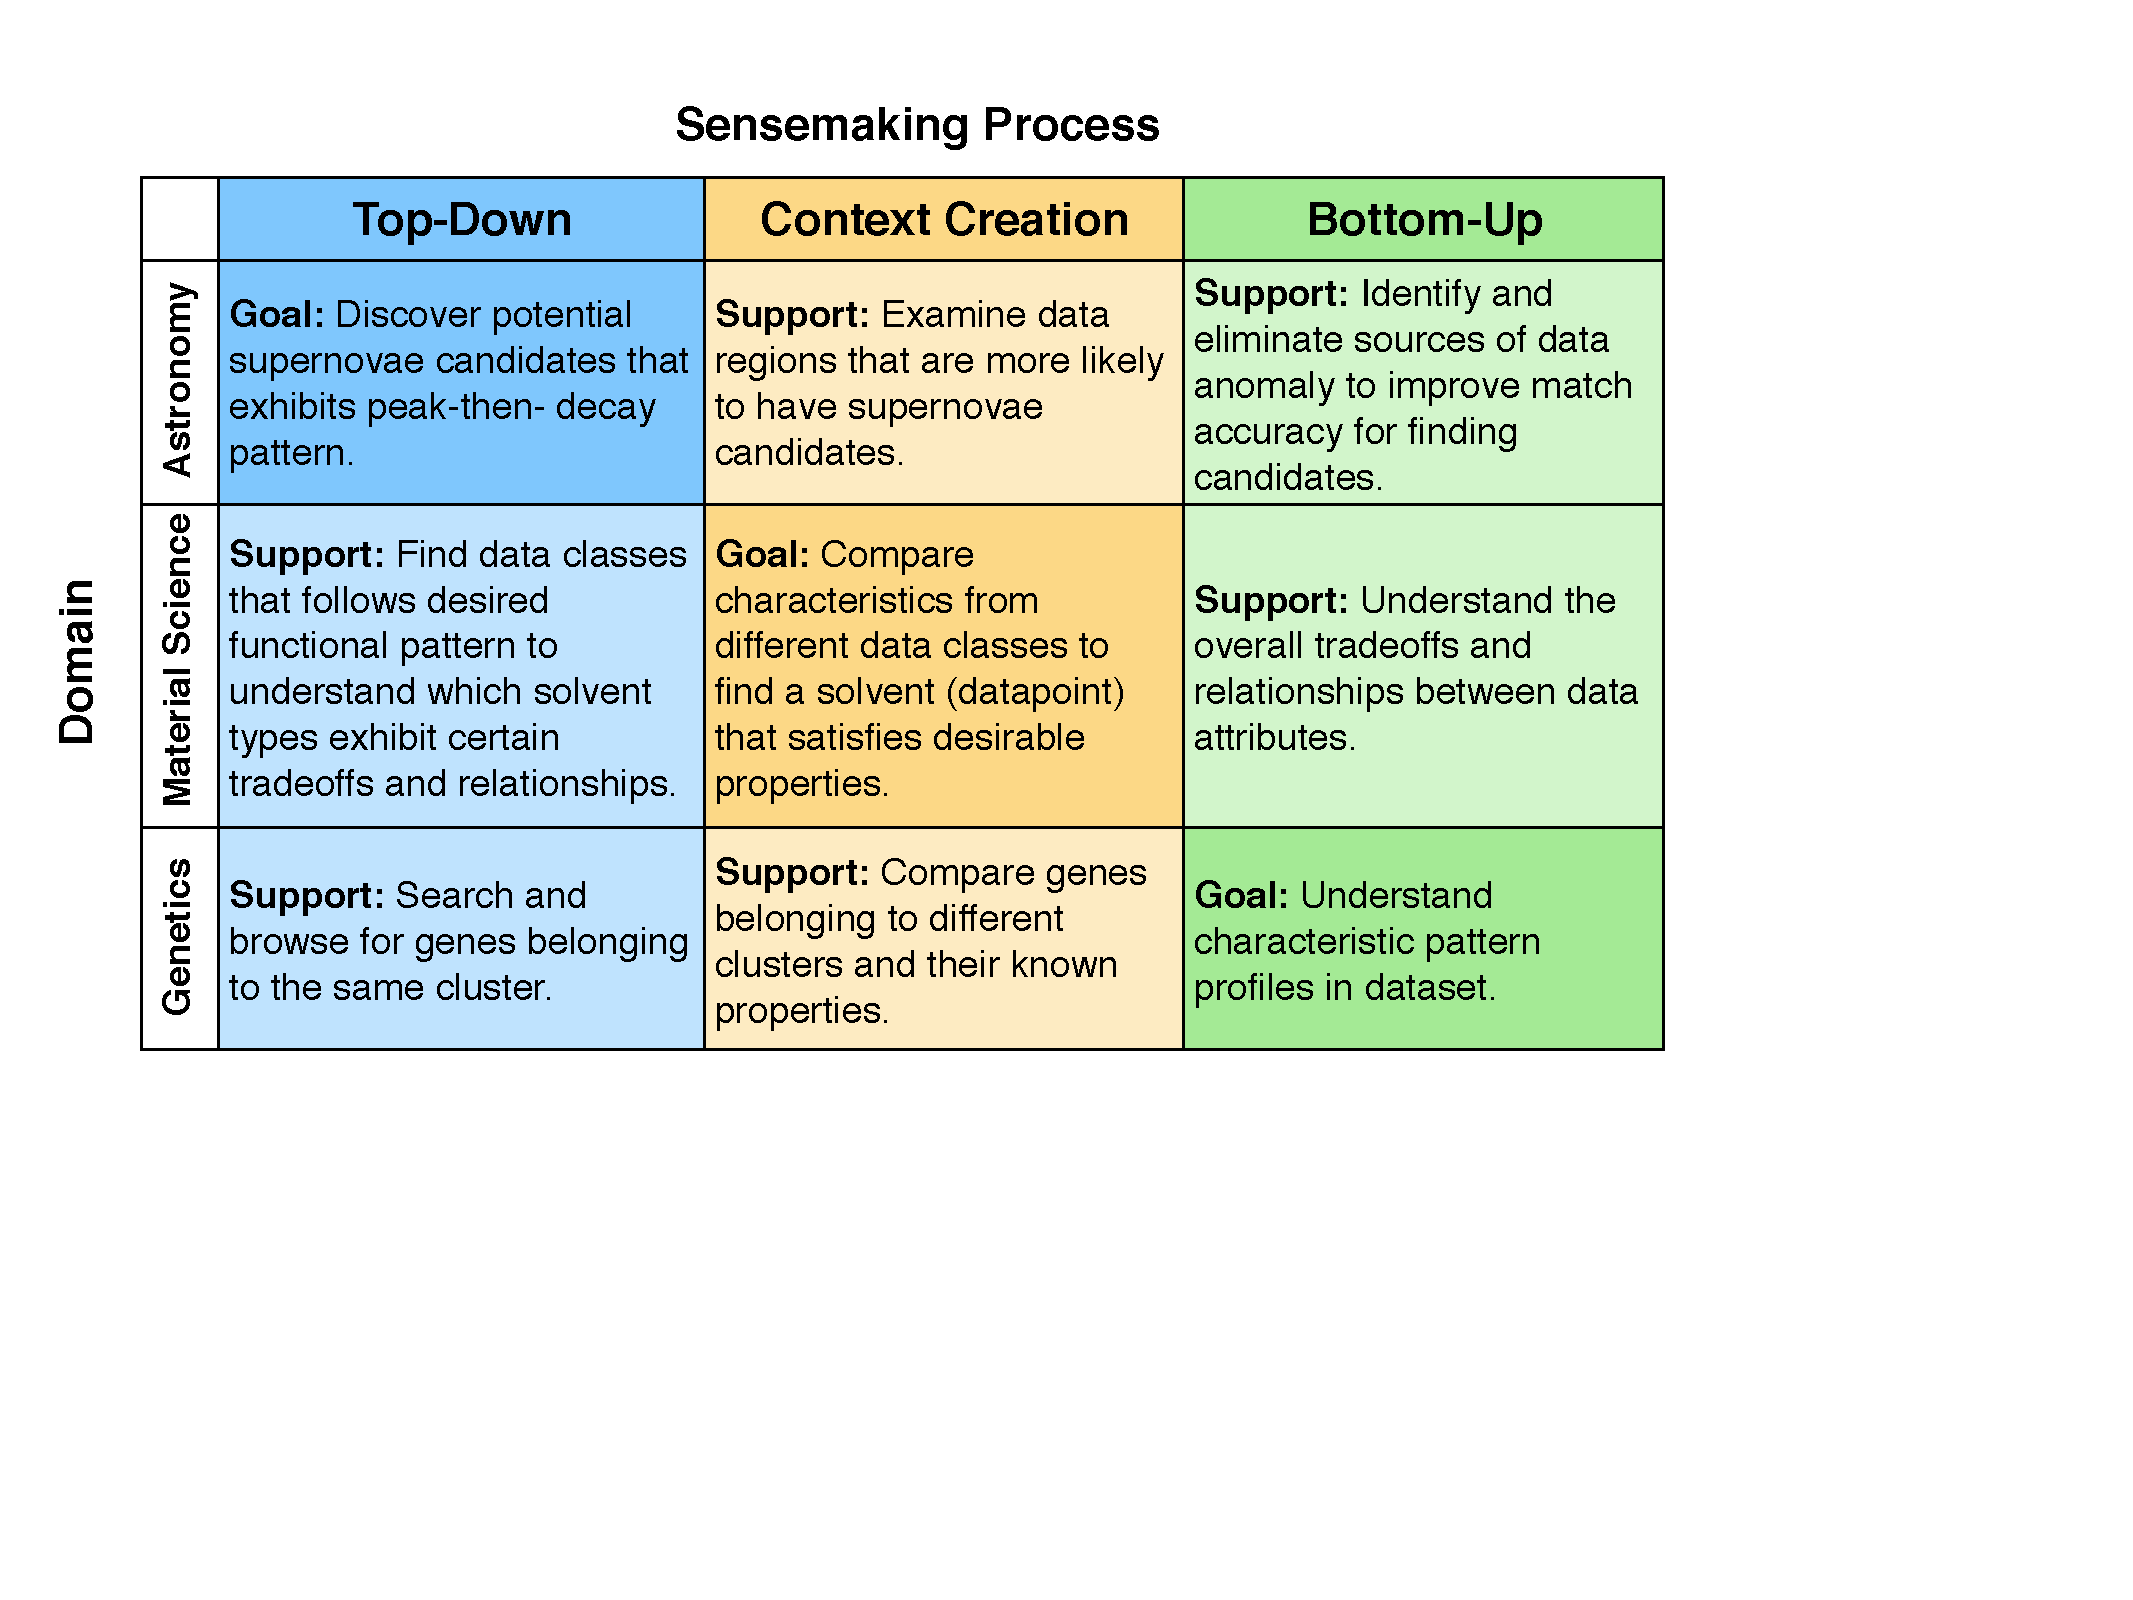
\includegraphics[width=\linewidth]{figures/science_task.pdf}
   \vspace{-6pt}\caption{\change{Each VQS sensemaking process maps to scientific tasks and goals from each use case, from pattern search to comparing visualization collections to gaining overall data understanding. We find that our scientific participants typically have one focused goal expressible through a single sensemaking process, but since their desired insights may not always be achievable with a single operation, they make use of the two other sensemaking processes to support them in accomplishing their main goal.}}
   \label{science_task}
   \vspace{-10pt}
\end{table}
% We provide usage scenarios to exemplify how each sensemaking process enables essential subtasks towards our participants' scientific goals (further detailed in  Table~\ref{science_task} in Appendix~\ref{apdx:pdartifact}).
 %\npar Table~\ref{science_task} illustrates how each of the subtasks in participant's workflow can be addressed by a sensemaking process.
   %ahen the visualized attributes are unknown to the users
 %, then we outline the design challenge addressed by each of the functional components that supports the sensemaking process
   % In this section, we first describe the space of problems addressable by VQSs.
   % After understanding how each sensemaking process fits into the problem space addressable} by VQSs,
   %  we further explore design objectives of each sensemaking process, grounded in our collaborative design experience.
   \subsection{Top-Down Pattern Search}
   Top-down processes are ``\textit{goal-oriented}'' tasks that makes use of ``\textit{analysis or re-evaluation of theories [and] hypotheses [to] generate new searches}''~\cite{Pirolli}. Applying this notion to the context of VQSs, the goal of top-down pattern search is to search for data instances that exhibit a specified pattern, based on analyst's intuition about how the desired patterns should look like ``in theory'' (including visualizations from past experience or abstract conceptions based on external knowledge). Based on this preconceived notion of what patterns to search for, the design challenge is to translate the pattern query from the analyst's head to a query executable by the VQS. This requires both components for specifying the pattern (\textit{pattern specification}), as well as controls governing how the pattern-matching is performed (\textit{match specification}).
   %address the \textit{which} question of visual sensemaking: \textit{which data instances exhibit this pattern?}
   %%%%%%%%%%%%%%%%%%%%%%%%Components%%%%%%%%%%%%%%%%%%%%%%%%%%%%
   \boldpara{Pattern Specification} interfaces allow users to submit exact descriptions of a pattern query. This is useful when the dataset contains \emph{large numbers of potentially-relevant pattern instances}.
   Since it is often difficult to sketch precisely, additional characteristics of the pattern query (e.g., patterns with specific shape characteristics, or expressible in a functional form) can be used to further winnow the list of undesired matches.%with the VQS returning a list of most similar matches
   \boldpara{Match Specification} addresses the well-known problem in VQSs where pattern queries are imprecise~\cite{correll2016semantics,Holz2009,Eichmann2015} by enabling users to clarify how pattern matching should be performed. Match specification is useful when the dataset is \emph{noisy}. When the pattern query satisfies some additional constraints (e.g., the pattern is x,y invariant), adjusting these knobs helps prune away matches that are false-positives to help analysts discover true desired candidates.
   \boldpara{Usage Scenario:} A1 knows intuitively what a supernovae pattern should look like and its detailed shape characteristics, such as the amplitude of the peak and the level of error tolerance for defining a match. He performs top-down pattern search by querying for transient patterns through sketching and adjusting the match criterion by choosing to ignore differences along the temporal dimension and changing the similarity metric for flexible matching.
   \subsection{Bottom-Up Data-Driven Inquiry}%goes from data to theory to
   In Pirolli and Card's sensemaking model, bottom-up processes are ``\textit{data-driven}'' tasks initiated by ``\textit{noticing something of interest in data}''~\cite{Pirolli}. Likewise in VQSs, bottom-up data-driven inquiry is a browsing-oriented sensemaking process that involves tasks that are inspired by system-generated visualizations or results. The design challenge for VQSs to support bottom-up data-driven inquiries is to develop the right set of ``stimuli'' through \textit{recommendations} that could provoke further data-driven inquiries, as well as low-effort mechanisms to search via these results through \textit{result querying}. As we will discuss later, this process is crucial but underexplored in past work on VQSs. %addresses the \textit{what} questions in visual sensemaking: \textit{what are the patterns of interest in the dataset?}
   %%%%%%%%%%%%%%%%%%%%%%%%Components%%%%%%%%%%%%%%%%%%%%%%%%%%%%
   \boldpara{Recommendations} display visualizations that may be of interest to users based on the current data context. In \zvpp, recommendations comprise of representative trends and outliers, which are useful for understanding common and outlying behaviors when a \emph{small number of common patterns} is exhibited in the dataset. %Understanding \emph{characteristic} patterns in dataset can help analysts discover other pattern queries of interest to jumpstart further queries.
   \boldpara{Result querying} enables users to query for patterns similar to a selected data pattern from the ranked list of results or recommendations. Typically, analysts select visualizations with \emph{semantic or visual properties} of interest and make use of result querying to understand characteristic properties of similar instances.
   \boldpara{Usage Scenario:} G2 does not have a preconceived knowledge of what to search for in the dataset. She engages with bottom-up data-driven inquiries to learn about the characteristic patterns that exist in the dataset through representative trends, as a means to jump-start further queries via result querying, as well as to understand groups of data instances with shared characteristics.
   \subsection{Context creation}
   While top-down and bottom-up processes operate on a collection of visualizations with fixed X and Y attributes, context creation operates in the regime where the analyst may be investigating the relationships between multiple different attributes of interest. Context creation enables analysts to navigate across different visualization collections to learn about patterns in different regions of the data. The design challenge of context creation is to help users visualize and compare how data changes between \change{these} different contexts by constructing visualization collections with different visual encodings (\textit{view specification}) or different data subsets (\textit{slice-and-dice}).%to ensure that context is dynamically reflected across other VQS functionalities through
   %develop features that act as a `lens': navigating users to desired data subsets, visualizing and comparing how the data changes between the different lenses, and ensuring that context is dynamically reflected across other VQS functionalities.
   %%%%%%%%%%%%%%%%%%%%%%%%Components%%%%%%%%%%%%%%%%%%%%%%%%%%%%
   \boldpara{View specification} settings alter the encoding for all of the visualizations on the VQS currently being examined. This ability to work with different collections of visualizations is useful when the dataset is \emph{multidimensional} and the axes of interest are \emph{unknown}. Modifying the view specification offers analysts different perspectives on the data to locate visualization collections of interest.
   \boldpara{Slice-and-Dice} empowers users to navigate and compare collections of visualizations constructed from different subselections of the data. Data navigation capabilities is essential when the dataset has \emph{large numbers of ``support attributes''} that may be related to the visualization attributes (e.g., geographical location may influence the time series pattern for housing prices). Analysts can either make use of pre-existing knowledge regarding these support attributes to navigate to a data region that is more likely to contain the desired pattern (e.g., filtering to suburbs to find cheaper housing) or discover unknown patterns and relationships between different data subsets (e.g., housing prices are lower in winter than compared to summer).% by gaining a better understanding of characteristic patterns in particular data region.
   \boldpara{Usage Scenario:} M1 recognizes salient trends in his dataset such as inverse or linear correlations, but does not have fixed attributes that he wants to visualize or a pattern in mind to query with. Given a list of physical properties of potential interest, he performs context creation by switching between different visualized attributes to understand the dataset from alternative perspectives. He can also dynamically create different classes of data (e.g., solvents with low solubility or have high capacity) to examine their aggregate patterns.
   \par The three aforementioned sensemaking processes are akin to the well-studied sensemaking paradigms of search (top-down), browse (bottom-up), and faceted navigation (context creation) on the Web~\cite{Hearst2009,Olston2003}. Due to each of their advantages and limitations given different information seeking tasks, search interfaces have been designed to support all three complementary acts and transition smoothly between them to combine the strength of all three sensemaking processes. Similarly for VQSs, our design objective is to enable all three sensemaking processes in \zvpp. Our Section~\ref{sec:eval_findings} evaluation study reveals that this integrative approach not only accelerates the process of visualization discovery, but also encourages hypotheses generation and experimentation.
 
%!TEX root = main.tex
 \section{Evaluation Study Findings\label{sec:eval_findings}}
 % \begin{figure*}[t!]
 % \minipage{0.6\textwidth}
 %   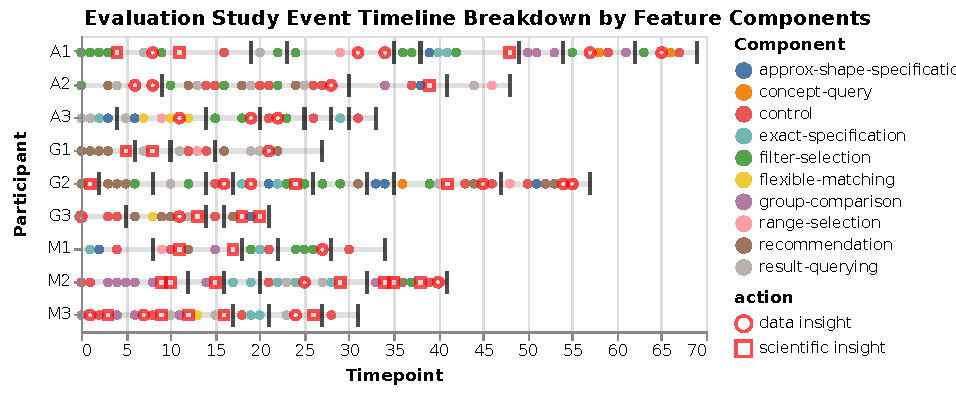
\includegraphics[width=\linewidth]{figures/evalstudytimeline.pdf}
 %   \caption{Timeline of event code and component usage, with every timepoint as an event on the x axis. For clarity, we hide most of the event coding labels other than the insight labels. Black vertical tick indicates a session break, signaling the beginning of a new line of inquiry.}\label{fig:evalstudytimeline}
 % \endminipage\hfill
 % \minipage{0.4\textwidth}
 %   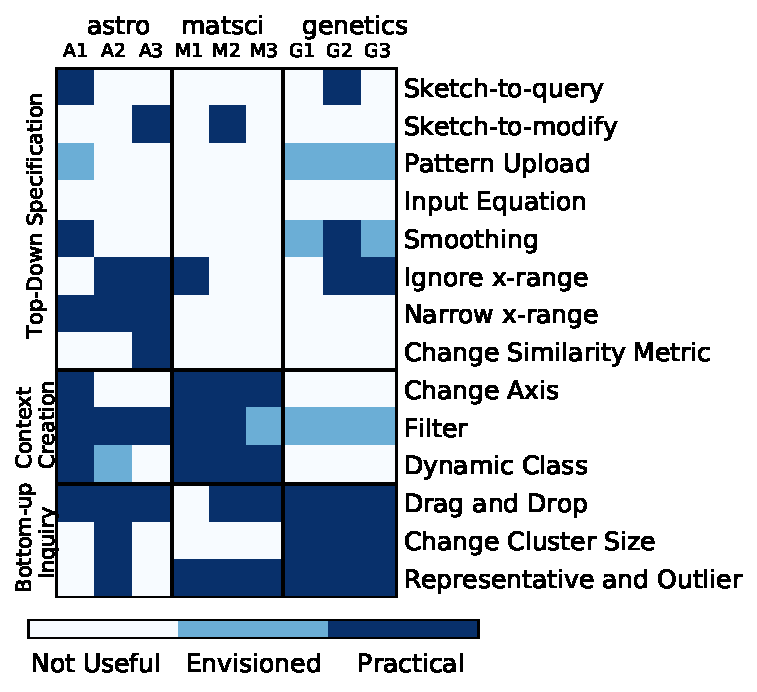
\includegraphics[width=0.8\linewidth]{figures/PENcoding.pdf}
 %   \caption{Heatmap of features categorized as practical usage (P), envisioned usage (E), and not useful (N).  \techreport{We find that participants preferred to query using bottom-up methods such as drag-and-drop over top-down approaches such as sketching or input equations. Participants found that data faceting via filter constraints and dynamic class creation were powerful ways to compare between subgroups or filtered subsets. The columns are arranged in the order of subject areas and the features are arranged in the order of the three foraging acts.}}\label{fig:feature_heatmap}
 % \endminipage
 % \end{figure*}
 Based on audio, video screen capture,
 and click-stream logs recorded
 during our \change{Phase II} evaluation study,
 we performed thematic analysis via open coding to label every event with a descriptive code. Event codes included specific feature usage,
 insights,
 provoked actions, confusion,
 need for capabilities unaddressed
 by the system, and use of external tools \achange{(see Appendix~\ref{apdx:studydetails} for details on our coding protocol)}. To characterize the usefulness
 of each feature, we further labeled whether each
 feature was useful to a particular participant's analysis.
 A feature was deemed \textit{useful}
 if the feature was either used in a sensible
 and meaningful way \change{to accomplish a task or address a question} during the study,
 or has envisioned usage outside of the constrained
 time limit during the study
 (e.g., if data was available or downstream analysis was conducted).
 We derived these labels from the study transcript
 to circumvent self-reporting bias~\cite{Williams2017},
 which can often artificially inflate
 the usefulness of the feature under examination.
 In this section, we will apply our thematic analysis results to understand how each sensemaking process occurs in practice.%real-world analytic tasks.}
 %\agp{Can't parse the previous sentence}
 %categorized the features based on whether there was a sensible usage of the feature
 % into one of the three usage types based on how each feature was used during the study:
 % \begin{denselist}
 %     \item Practical: Features used in a sensible and meaningful way.
 %     \item Envisioned: Features which could be used practically if the envisioned data was available or if they conducted downstream analysis, but was not performed due to the limited time during the study.
 %     \item Not useful: Features that are not useful or do not make sense for the participant's research question and dataset.
 % \end{denselist}
 % \par Given these initial findings, we further investigated where the `sketch'
 % Our interactions with the scientists showed that different modalities for inputting a query can be useful for different problem contexts. In addition, the three paradigms of sensemaking described earlier are not mutually exclusive. In fact, we find that participants often construct a central workflow focused on features from one of the main paradigms and interleave variations with the feature usage from the two other paradigms as they iterate on the analytic task. As shown in Figure~\ref{fig:usagefreqbysubject}, the central paradigm adopted by each use case is tightly coupled with characteristics of the analytic challenges presented by each subject area.
 % interplay
 % Next, we will describe some of the design principles (DP) based on our study findings.
 %focus on understanding the design space of VQSs and highlight the takeaways of our study.%developing a process model and design guideline for insight formation in VQSs and divert our thematic analysis of how VQSs fit into the context of an analysis workflow to our technical report.% These observation inform our ----- search-browse paradigm
 % \subsubsection{Discovery of Real-world insights}
 % \par Our participants' original workflow often required them to compare between many visualizations manually through separate analysis and visualization steps. Three of the participants cited that this segmented analyze-then-visualize workflow was one of their chief bottlenecks. The cognitive overhead from the segmented workflow made them more hesitant to visualize the results of different parameters and data operations, as A2 noted:
 % \begin{quote}
 % The quick visualization is something that I could not do on my current framework. I could not query as fast as you do; I need to wait for it, plot, and then compare. Every time I plot, I need to define subplots for 12 visualizations, then its slower. That's the reason why I sometimes plot less, and I rely more on the statistics from the likelihood tests. Sometimes I plot less than I really should be doing.
 % \end{quote}
 % The ability to rapidly experiment with large numbers of hypotheses in real time is a crucial step in the agile creative process in helping analysts discover actionable insights~\cite{Shneiderman2007a}. Five out of nine participants discussed how the dynamic, interactive update of the visualization in \zv was the main advantage for using VQSs over their original workflow.
 % \begin{figure}[h!]
 %   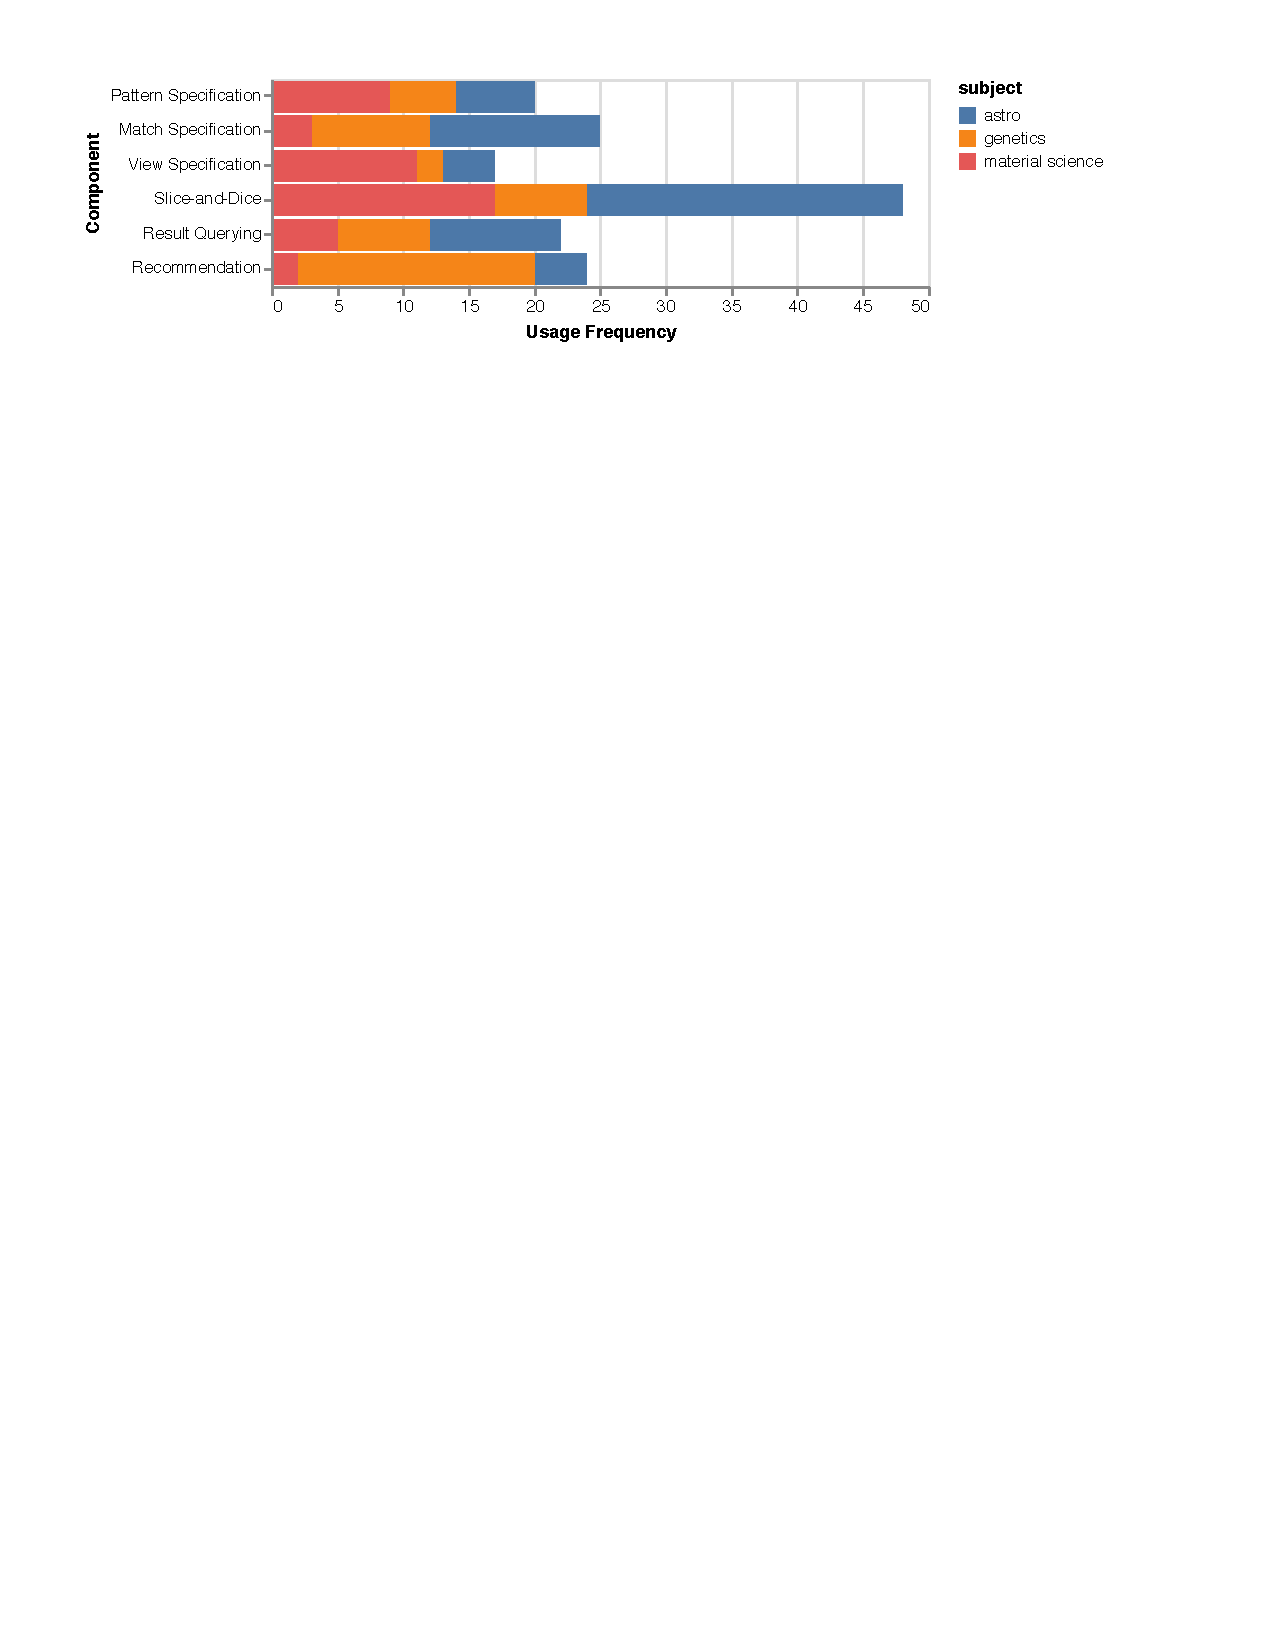
\includegraphics[width=\linewidth]{figures/usagefreqbysubject.pdf}
 %   \caption{The number of times each component is used during the evaluation study, broken down by subject areas.}\label{fig:usagefreqbysubject}
 % \end{figure}
 % \subsection{The Ineffectiveness of Sketch}
 \subsection{\change{Uncovering the Myth of Sketch-to-Insight}}
 % \subsection{DC3: Closing the loop in VQS sense-making cycle with bottom-up data-driven inquries}
 \par \change{To understand the usefulness of different visual querying modalities, we analyzed their frequency of use in our evaluation study.} To our surprise,
 despite the prevalence of sketch-to-query
 systems in the literature, \techreport{Figure \ref{fig:feature_heatmap} shows that} only two out of our nine participants
 found it useful to directly
 sketch a desired pattern onto the canvas. %Overall, bottom-up querying via drag-and-drop was more intuitive and more commonly used than top-down querying methods, such as sketching or input equations.
 The reason why most participants
 did not find direct sketching useful was that
 they often do not start their analysis with a specific pattern in mind.
 Instead, their intuition about what to query is derived
 from other visualizations they \change{encountered}
 during exploration, in which case it makes
 more sense to query using those visualizations
 as examples directly (e.g., by dragging and dropping
 that visualization onto the canvas to submit the query).
 Even if a user has a pattern in mind,
 translating that pattern into a sketch is often hard
 to do. For example,
 A2 wanted to search for a highly-varying signal
 enveloped by a sinusoidal pattern indicating
 planetary rotation 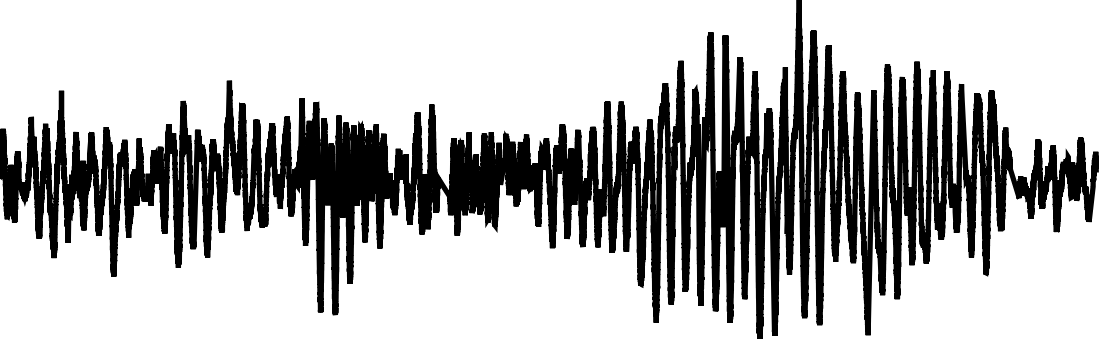
\includegraphics[width=2\baselineskip,keepaspectratio]{figures/impossible_sketch.png}, which \achange{was} hard to draw by hand.
 \begin{figure}[h!]
   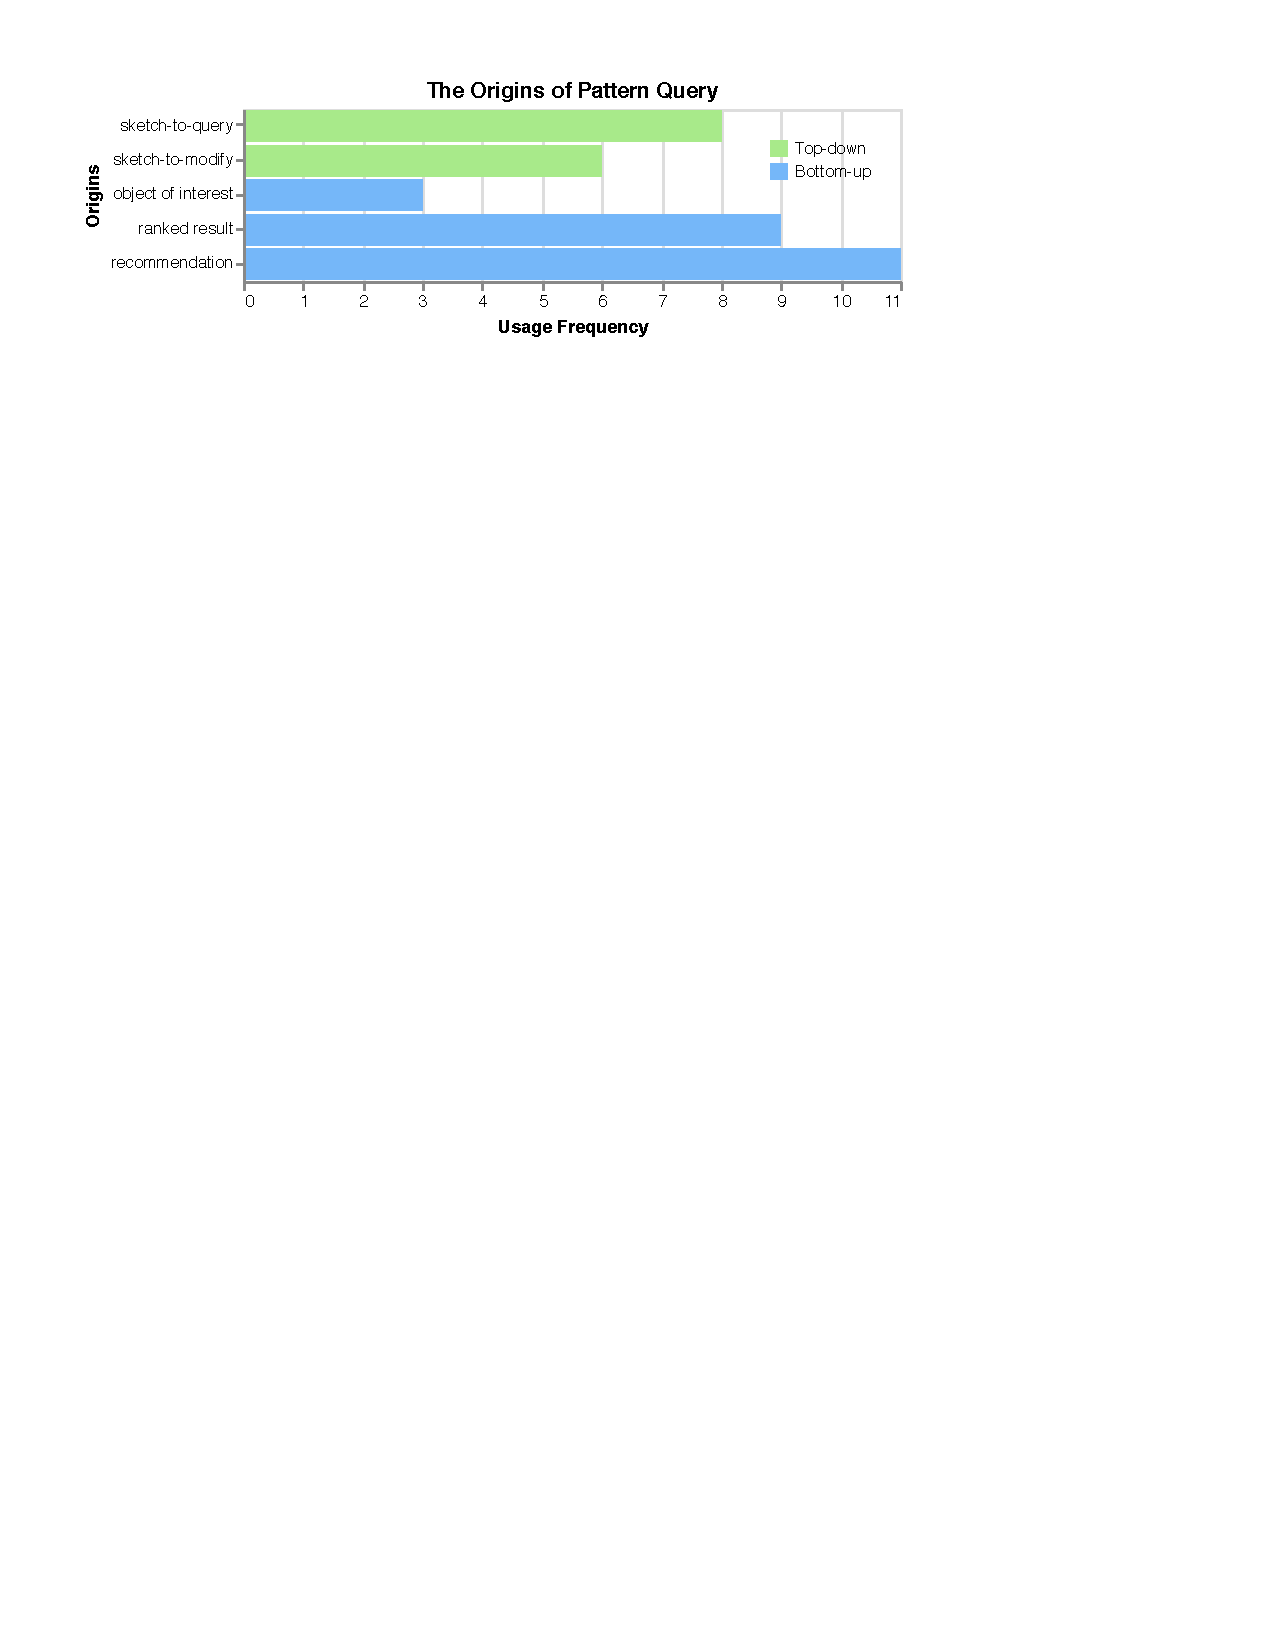
\includegraphics[width=0.95\linewidth]{figures/the_origins_of_sketch.pdf}
   \vspace{-5pt}
   \caption{The number of times a pattern query originates from one of the workflows. We find that pattern queries are far more commonly generated via bottom-up than top-down processes.}\label{fig:origins_of_sketch}
   \vspace{-5pt}
 \end{figure}
 %where the pattern on the canvas typically originates
 \par Given these initial findings,
 we further investigated \achange{the processes that participants engaged in to} construct pattern queries, as presented in Figure~\ref{fig:origins_of_sketch}.
 Pattern queries can be generated by
 either top-down (sketching) or
 bottom-up (drag-and-drop) processes,
 driven by various different querying intentions.
 Within top-down processes,
 a pattern query could arise
 from users directly sketching
 a new pattern (\bartext{sketch-to-query})
 or by modifying an existing sketch (\bartext{sketch-to-modify}). For example, M2 first sketched a pattern
 to find solvent classes with anticorrelated
 properties without much success in returning a desired match.
 %However, the sketched query did not return visualizations of interest.
 So he instead dragged and dropped one
 of the peripheral visualizations similar
 to his desired visualization and then smoothed
 out the noise in the visualization via sketching yielding
 a straight line,
 as shown in Figure \ref{query_modification} (left).
 M2 repeated this workflow twice in separate
 occurrences during the study and
 was able to derive insights from the results.
 Likewise, Figure~\ref{query_modification} (right)
 illustrates how A3 first picked out a regular pattern
 (suspected starspot), then modified it slightly
 so that the pattern looks more irregular (to find pulsating stars).
 %Within these actions, there can be different intentions behind the sketch. While all visualizations that could be drag-and-dropped must come from the result or recommendation pane, a query can come from a particular object that the participant is interested in or simply through peripheral browsing of visualization results.%, described in the next section.
 %\par The latter case is also supported by the
 %\par There are also many unexpected use cases where sketching was simply used as a mechanism to modify an existing pattern query.
 %Likewise, A3 was interested in pulsating stars that looked similar to stellar hotspots in terms of its dramatic amplitude fluctuations, but differ in that their patterns exhibited irregularities. Figure \ref{query_modification} (right) showed how she first picked out a regular pattern (suspected star spot), then modified it slightly so that the pattern looks more irregular.
 %Likewise, A3 was interested in pulsating stars characterized by dramatic changes in the amplitudes of the light curves. During the search, hotspots on stellar surfaces often show up as false positives as they also result in dramatic amplitude fluctuations, but happen at a regular intervals. In the VQS, A3 looked for patterns that exhibits amplitude variations, but also some irregularities. As shown in Figure \ref{query_modification} (right), she first picked out a regular pattern (suspected star spot), then modified it slightly so that the pattern looks more irregular.\par While all visualizations that could be drag-and-dropped must come from the result or recommendation pane, a query can come from a particular object that the participant is interested in or simply through peripheral browsing of visualization results.
 As described in the following section,
 bottom-up pattern queries can come from either
 the ranked list of results,
 recommendations, or by selecting a
 particular object of interest as a drag-and-drop query.
 Figure~\ref{fig:origins_of_sketch} shows that
 \emph{bottom-up processes are more common
 than top-down processes for generating a pattern query}.
 \begin{figure}[h!]
     \centering
     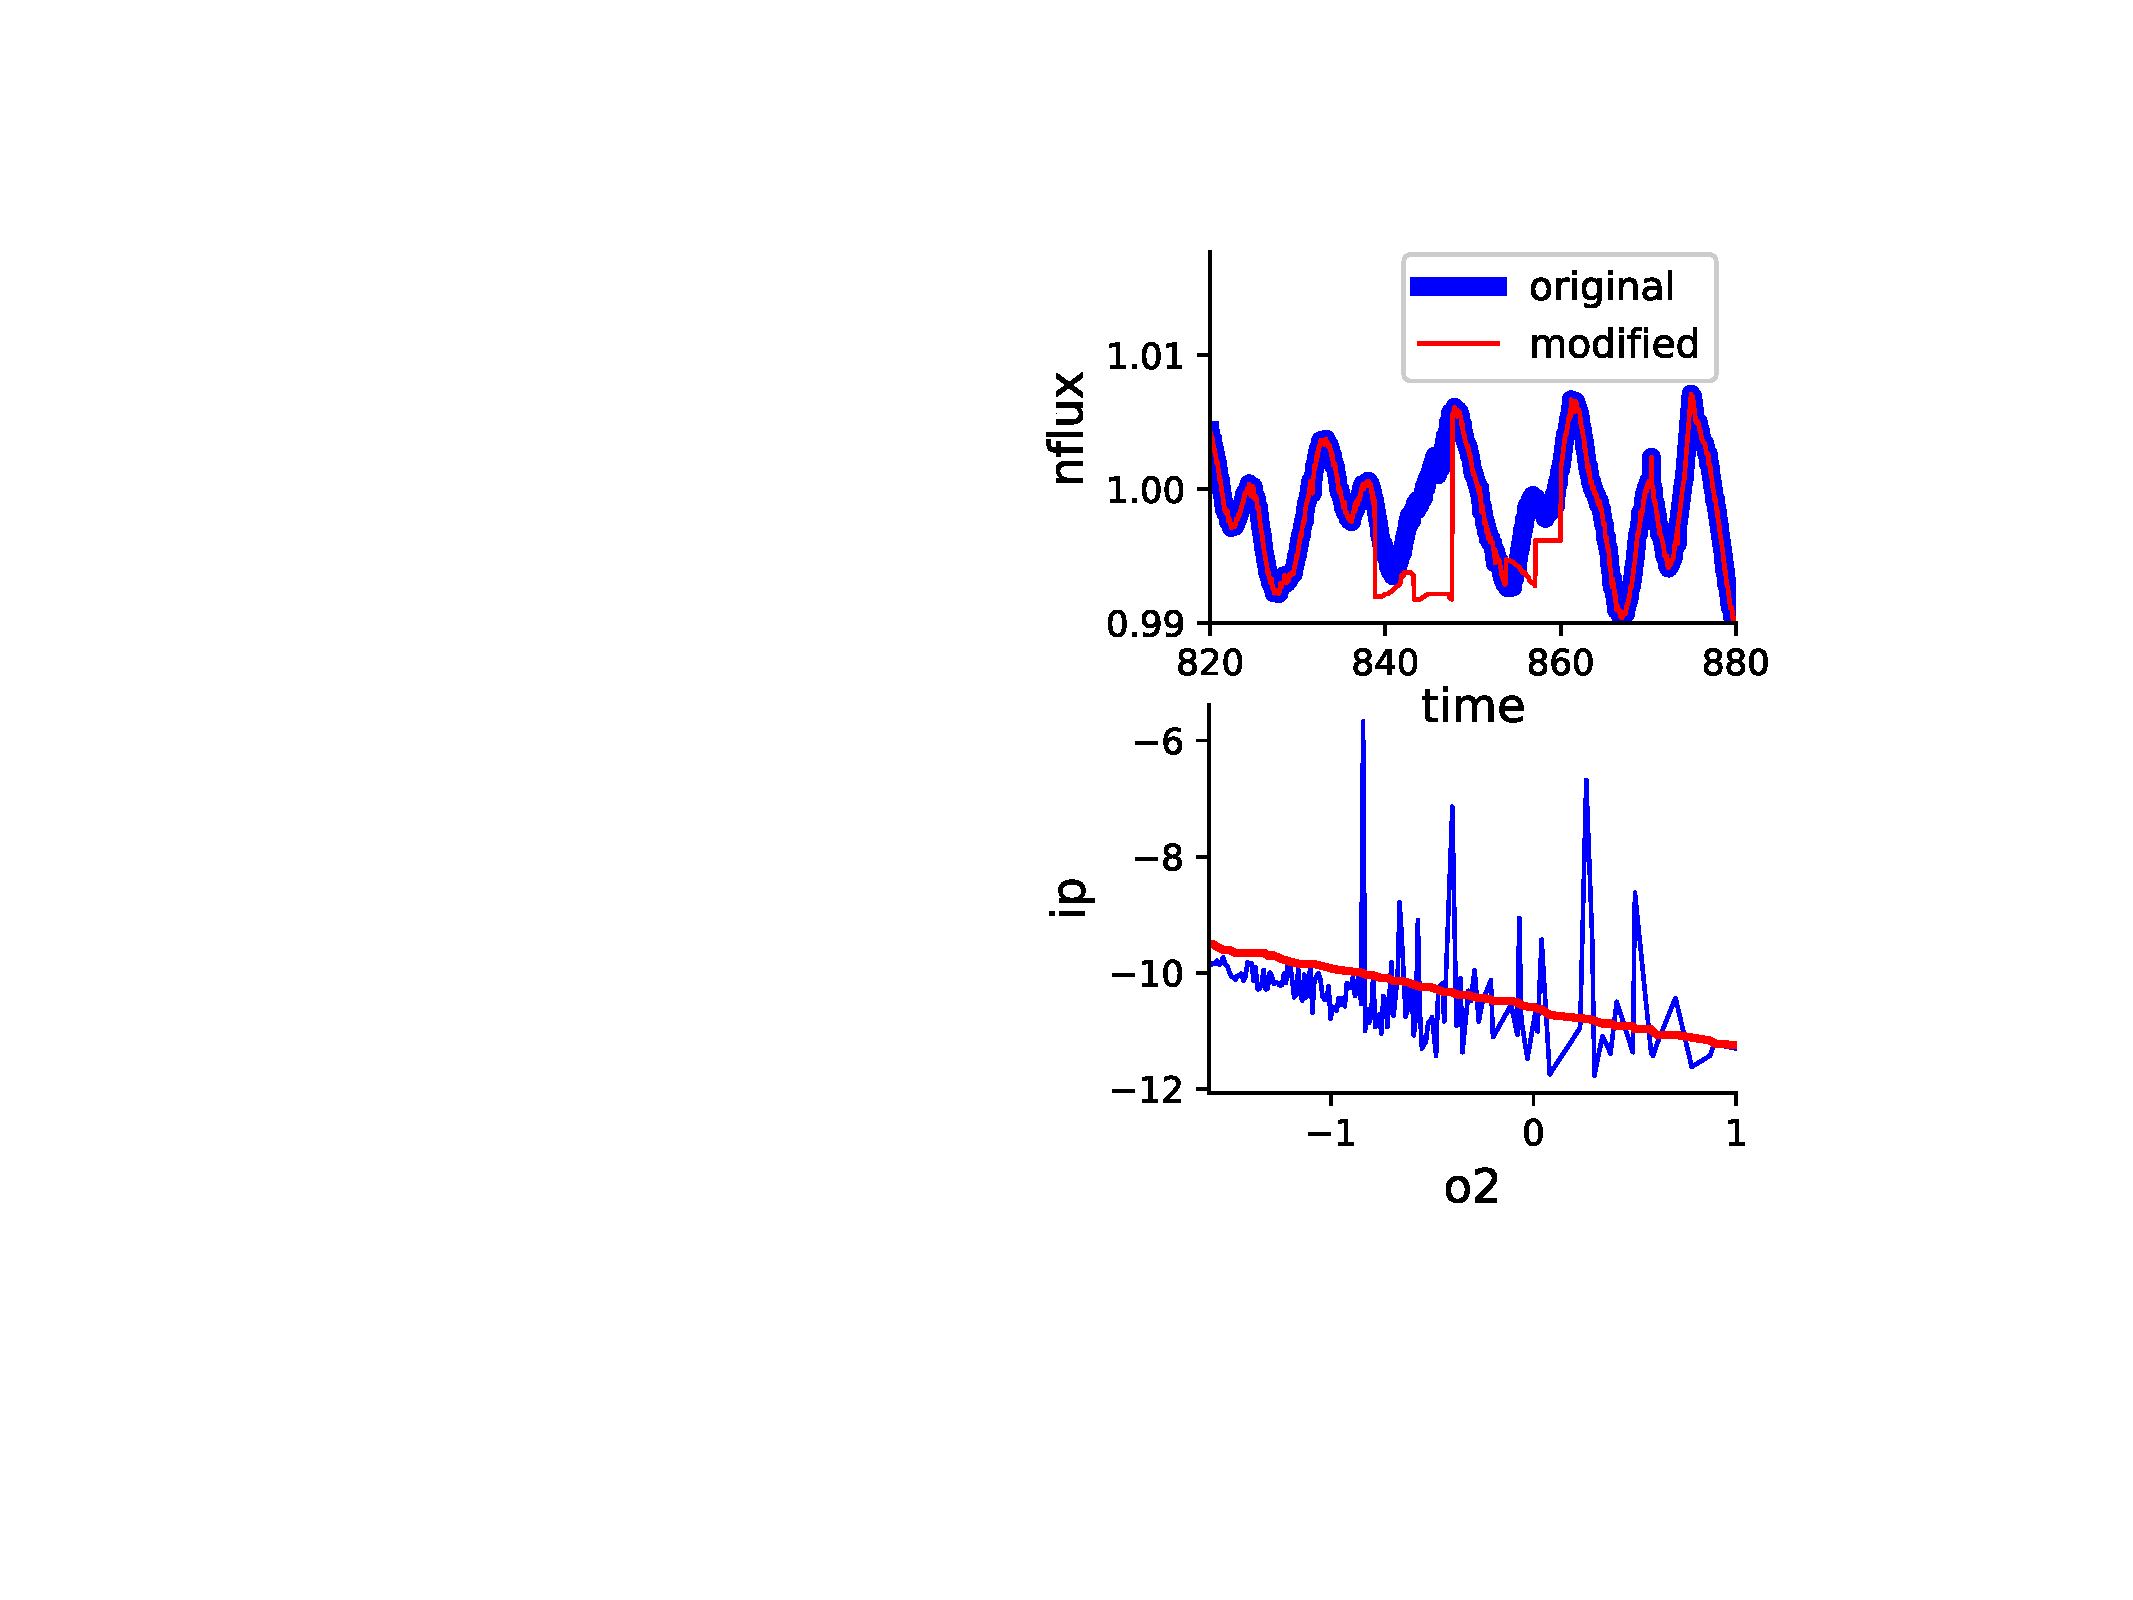
\includegraphics[width=\columnwidth]{figures/QueryModificationBySketch.pdf}
     \caption{Example of sketch-to-modify, based on canvas traces from M2 (left) and A3 (right). The original drag-and-dropped query is shown in blue and sketch-modified queries in red.}%during the study demonstrating query modification
     \label{query_modification}
     \vspace{-10pt}
 \end{figure}
 \par The \achange{infrequent use of top-down pattern
 specification was} also reflected in the fact
 that none of the participants queried using an equation.
 In both astronomy and genetics, the visualization patterns
 resulting from complex physical processes
 that could not be written down as an equation analytically.
 Even in the case of material science when analytical
 relationships do exist, it is challenging to formulate patterns as functional forms in a prescriptive manner.
 % Despite functional fitting being common in scientific data analysis, Figure \ref{feature_heatmap} shows that
 % . However,
 \par Our findings suggest that while sketching
 is a useful construct for people to express their queries,
 \emph{the existing ad-hoc, sketch-only model for VQSs
 is insufficient \change{on its own}} without data examples
 that can help analysts jumpstart their exploration.
 In fact, from Figure~\ref{fig:origins_of_sketch},
 we can see that sketch-to-query was only used
 8 times, while the remaining querying modalities were used 29 times altogether,
 more than three times as much as sketch-to-query.
 This finding has profound implications
 on the design of future VQSs, since Table~\ref{table:relatedwork}
 suggests that past work has primarily focused
 on optimizing top-down process components,
 without considering how useful these features
 are in real-world analytic tasks.
 %missing out largely on the key components in the other two paradigms \cut{(indicated by the absence of green features on the right hand side of the table).
 We suspect that these limitations
 may be why existing VQSs are not commonly adopted in practice. \change{Note that we are not advocating for removing the \achange{natural and intuitive} sketch capabilities from future VQSs completely, but instead focusing future research and design efforts to examine other (often underexplored) VQS sensemaking processes. \achange{Such processes could be applied} in conjunction with sketching to help analysts more flexibly express their analytical goals, described next.}

 %This result points to a need for ----- in future VQSs. %This, however, points to an exciting direction for sketching interface in VQSs for developing advanced drawing and modification tools that enable more precise visualization query specification.} %ed coverage in addressing different types of analytics use cases
 %For instance, material science discovered a known inverse relationship during e xploration
 %Which is really interesting. Which is something that we observed experimentally also. That is an interesting insight right htere. This seems to suggest that there is a fundamental issue in if you want to try to get better on this axis, and get as low as possible, you lose out on the other axis.
 %once they see it they know it but they don't know beforehand
 
 \subsection{\change{Insights via Context Creation and Bottom-up Approaches}}%Approaches}
 % \dor{Might need to come up with a more descriptive name for this subsection}
 \par As alluded to earlier,
 \emph{bottom-up data-driven inquiries
 and context creation are far more commonly
 used than top-down pattern search
 when users have no desired patterns in mind},
 which is typically the case for exploratory data analysis.
 In particular, top-down approaches were only useful for 29\% of the use cases,
 whereas \change{they were} useful for 70\% of the use cases
 for bottom-up approaches and 67\%
 for context creation\footnote{See Appendix~\ref{apdx:studydetails} for details on how this measure was computed.}. We now highlight some exemplary workflows demonstrating the efficacy of the latter two sensemaking processes.
 %number of features labeled as useful divided by the product of total number of features and total number of users}
 %%The prevalence of bottom-up approaches not only point to the need for result querying, but also providing recommendations for users without desired patterns in mind.
 \par As shown in Figure~\ref{fig:origins_of_sketch} \achange{(\bartext{recommendations})},
 the most common use of bottom-up querying
 is via recommended visualizations. For example, G2 and G3 identified that
 the three representative patterns
 recommended in \zvpp corresponded
 to the same three groups of genes discussed
 in a recent publication~\cite{Gloss2017}:
 induced genes (profiles with expression levels going up 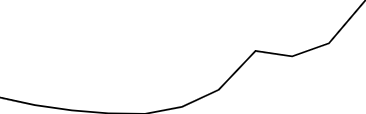
\includegraphics[width=2\baselineskip,keepaspectratio]{figures/induced.png}),
 repressed genes (starting high then decreasing 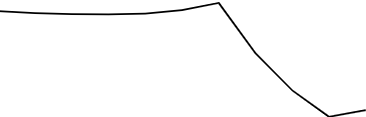
\includegraphics[width=2\baselineskip,keepaspectratio]{figures/repressed.png}),
 and transients (rising first then dropping at another time point 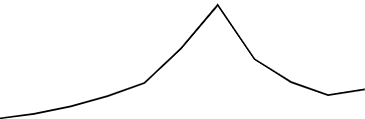
\includegraphics[width=2\baselineskip,keepaspectratio]{figures/transient.png}). The clusters provoked G2 to generate a hypothesis
 regarding the properties of transients:
 \textit{``Is that because all the transient groups
 get clustered together, or can I get sharp patterns
 that rise and ebb at different time points?''}
 To verify this hypothesis, G2 increased the parameter controlling the number of clusters and noticed that the clusters
 no longer exhibited the clean,
 intuitive patterns he had seen earlier.
 G3 expressed a similar sentiment and proceeded
 by inspecting the visualizations
 in the cluster via drag-and-drop.
 He found a group of genes that all transitioned
 at the same timestep, while others transitioned
 at different timesteps.
 \techreport{G3 described the process of using
 VQSs as doing ``detective work'' that provoked
 him to generate further scientific hypotheses
 as well as data actions.}
 \par By browsing through the ranked list of
 results \achange{(corresponding to the \bartext{ranked results} bar in Figure~\ref{fig:origins_of_sketch})}, participants were also able to
 gain a peripheral overview of the data
 and spot anomalies during exploration.
 For example, A1 spotted time series
 that were too faint to look like stars
 after applying the filter CLASS\_STAR=1,
 which led him to discover that all stars
 have been mislabeled with CLASS\_STAR=0 as 1 during data cleaning.
 %This includes inspecting the top-most similar visualizations that lie in the queried cluster. and finding visualizations that are similar to an object of interest that exhibits a desired pattern. %. After browsing through a series query results and checking with an external database, he concluded that
  %We found that geneticists often gain their intuition about the data from the recommended representative trends. One example of rapid insight discovery
 %the dataset had been incorrectly labelled with all the stars with CLASS\_STAR=0 as 1 during data cleaning.
 %Examples of how recommended trends can provoke further insightful actions comes from G2 and G3, who identified that the three representative patterns shown in \zvpp---induced genes (profiles with expression levels staying up), repressed genes (started high but went down), and transients (go up and then come down at different time points)---corresponded to the same three groups of genes discussed in a recent publication~\cite{Gloss2017}.
 % \subsection{Enriching Search with Context}
 \begin{figure*}[ht!]
   \centering
   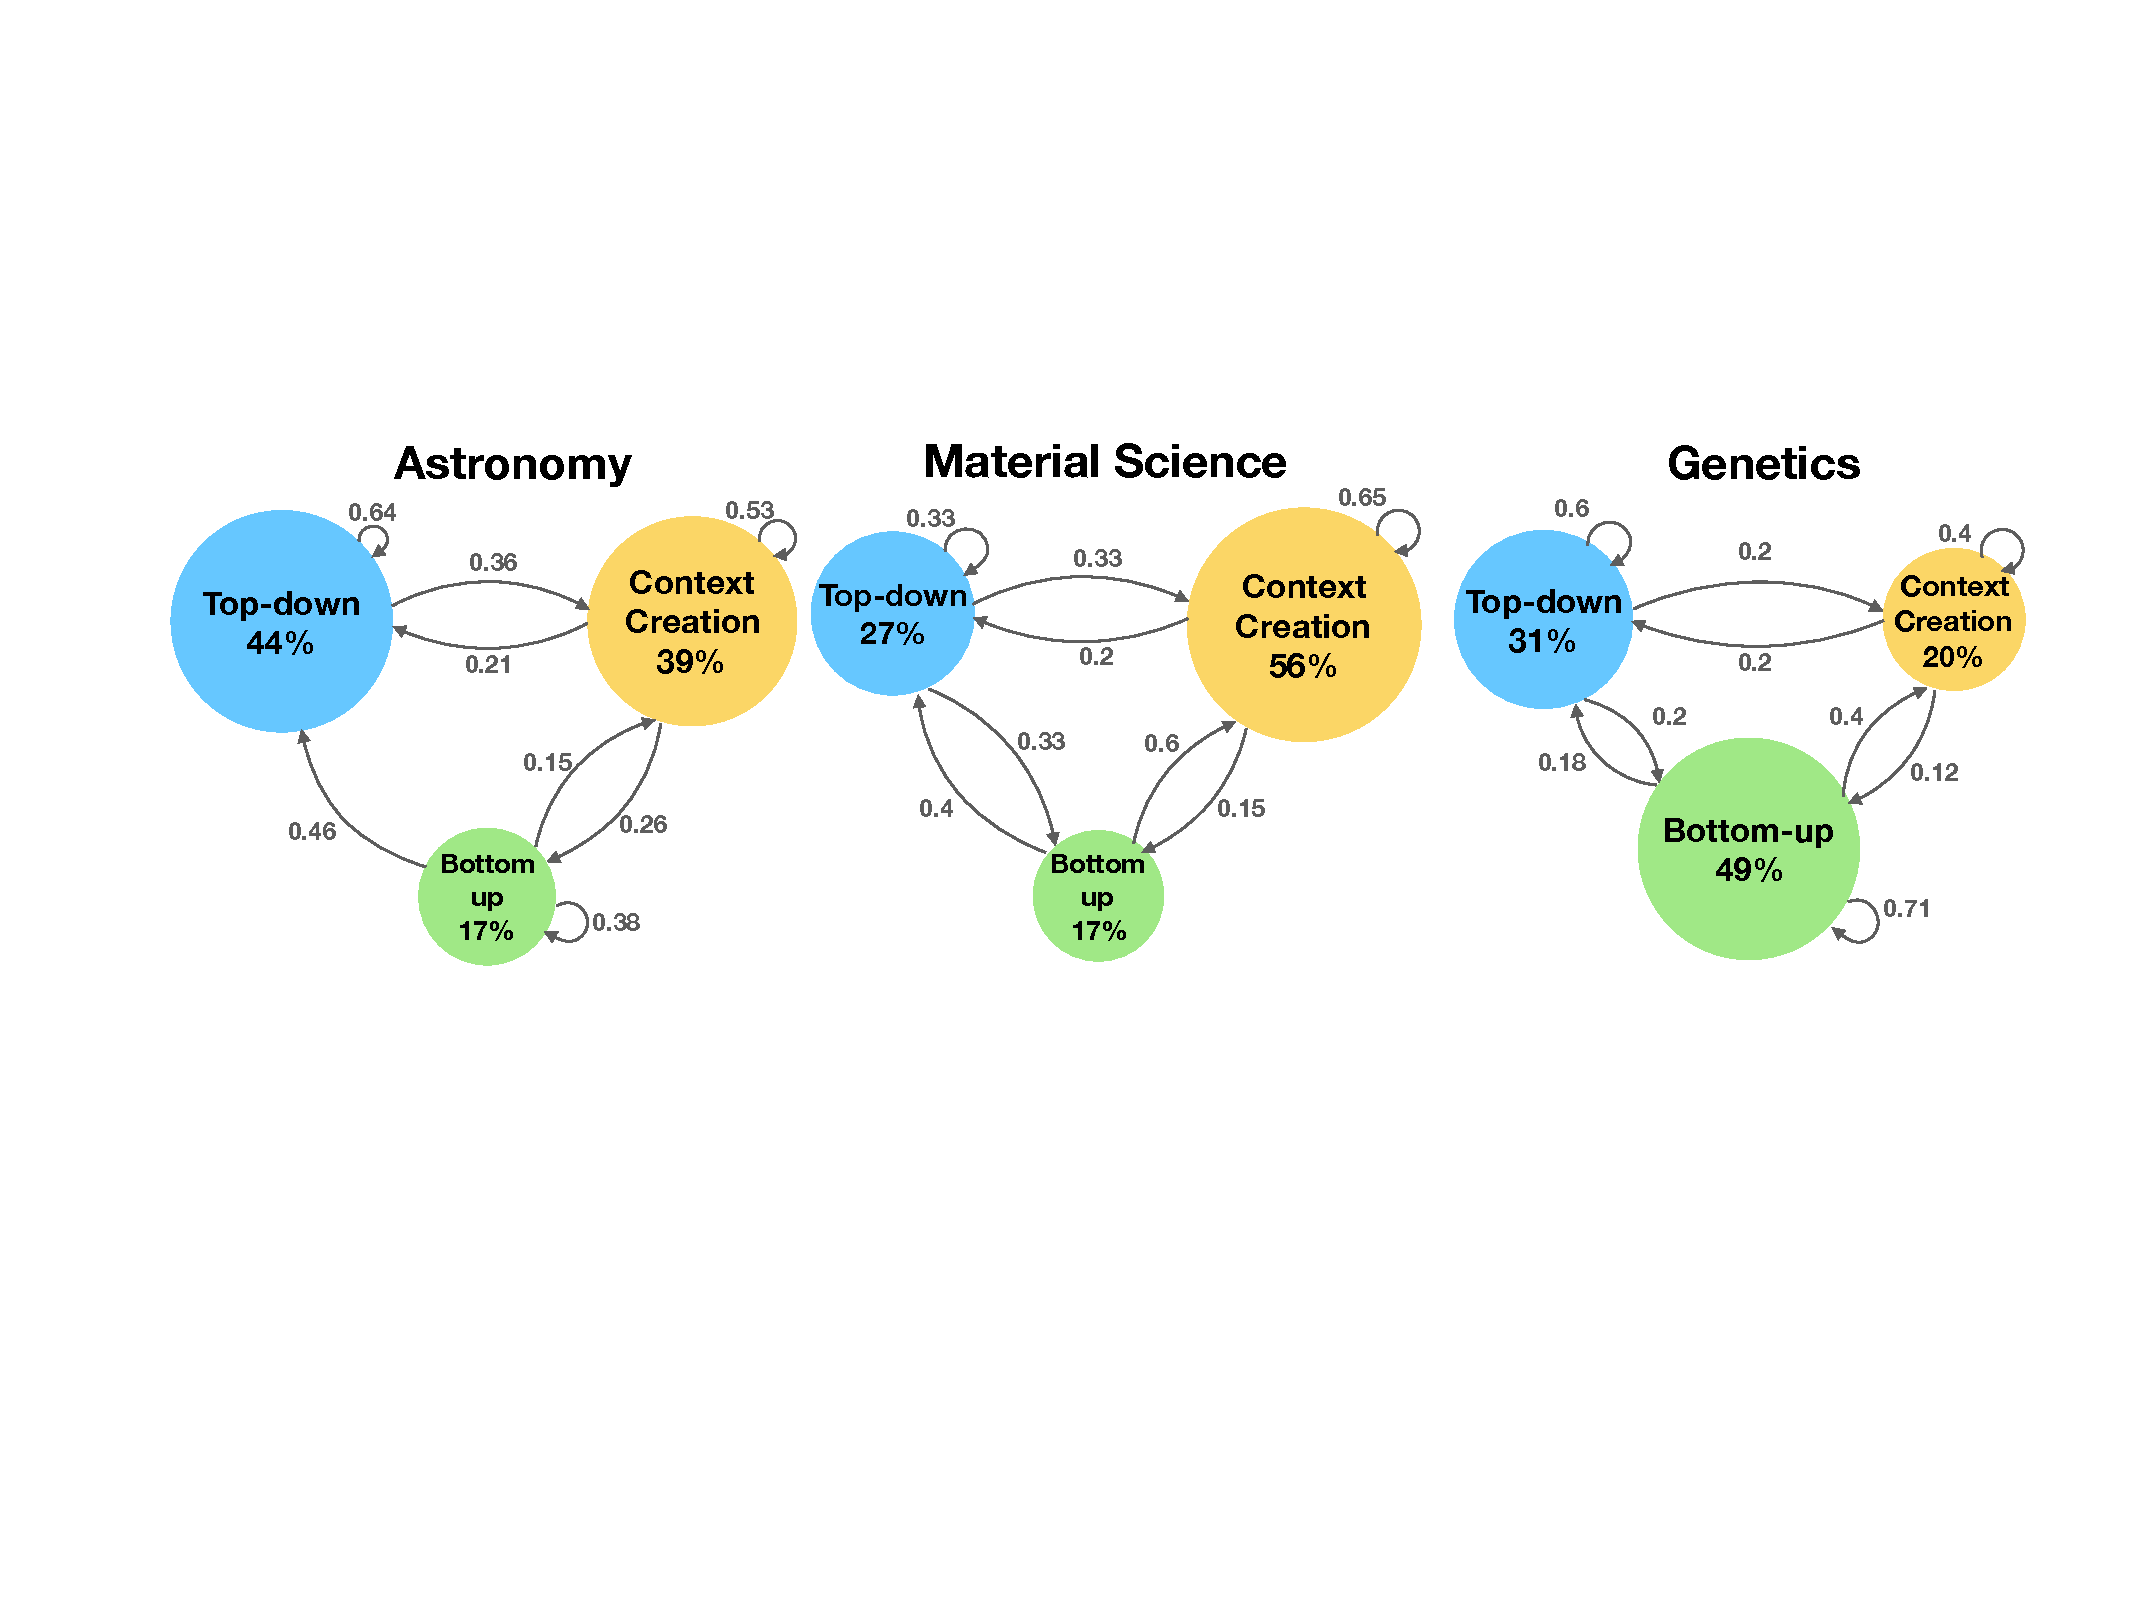
\includegraphics[width=0.6\linewidth]{figures/markov_transition.pdf}
   \caption{Markov models computed based on evaluation study event sequences, with edges denoting the probability that participant in the particular domain will go from one sensemaking process to the next. Nodes are scaled according to \change{their} eigenvector centrality, representing the percentage of time participants would spend in a particular sensemaking process in steady state. \achange{Markov models are computed based on a total of 206 event actions taken by participants during the evaluation study (80 for astronomy, 65 for genetics, and 61 for material science).}}\label{fig:transition}
   \vspace*{-15pt}
 \end{figure*}
 \par Past studies in visual analytics
 have shown that it is important to design features
 that enable users to select relevant subsets of data~\cite{Amar2005,Heer2012}.
 Context creation in VQSs enables users to change the ``lens''
 by which they look through the data
 when performing visual querying,
 thereby creating more opportunities
 to explore the data from different perspectives. All participants found at least
 one of the features in context creation to be useful.
 %We designed two dynamic faceting features coupled with coordinated views that enabled users to specify subsets of data they are querying on and see immediate changes updated in the query, representative, and outlier results.
 %either envisioned a use case or utilized features in the context creation paradigm to explore and compare subsets of their data.
 %ven though the filtering step could be easily done with an external tool and reloaded into \zv, filtering on-the-fly was a powerful way to dynamically test his hypothesis. I
 \par Both A1 and A2 expressed that context creation through interactive filtering enabled them to test conditions and tune values that they would not have otherwise modified, effectively lowering the barrier between the iterative hypothesize-then-compare cycle during sensemaking.
 % echoing our previous finding that segmented workflow prevents extensive exploration.
 During the study, participants used filtering
 to address questions such as:
 \textit{Are there more genes similar
 to a known activator when we subselect
 only the differentially expressed genes?} \techreport{\texttt{DIFFEXP=1} }(G2) or \textit{Can I find more supernovae candidates if I query only on objects that are bright and classified as a star?} \techreport{\texttt{flux\textgreater10 AND CLASS\_STAR=1} }(A1). Three participants had also used filtering as a way to query with known individual objects of interest, as shown in \achange{the \bartext{object of interest} bar of} Figure~\ref{fig:origins_of_sketch}. For example, G2 set the filter as gene=9687 and explained that since ``\textit{this gene is regulated by the estrogen receptor, when we search for other genes that resemble this gene, we can find other genes that are potentially affected by the same factors.}''
 \par While filtering enabled users to
 narrow down to a selected data subset,
 dynamic classes (buckets of data points that satisfies one or more range constraints) enabled users to compare
 relationships between multiple attributes and subgroups of data.
 For example, M2 divided solvents in the database
 into eight different categories based on voltage properties,
 state of matter, and viscosity levels,
 by dynamically setting the cutoff values
 on the quantitative variables to create these classes.
 By exploring these custom classes, M2 discovered that the relationship between viscosity and lithium solvation energy is independent of whether a solvent belongs to the class of high voltage or low voltage solvents. He cited that dynamic class creation was central to learning about this previously-unknown attribute properties:
 \begin{quote}
 All this is really possible because of dynamic class creation, so this allows you to bucket your intuition and put that together. [...] I can now bucket things as high voltage stable, liquid stable, viscous, or not viscous and start doing this classification quickly and start to explore trends. [...] look how quickly we can do it!% Quite good!
 \end{quote}
 %Context creation is a useful ---- despite the --- pattern instance. Filtering still useful
 %\par Participants employed \emph{a mix of bottom-up and top-down approaches when faceting through data in VQS}, including narrowing the search space based on some intuition about a phenomena, selecting individual visualizations, or specifying high-level groupings to compare and query with.
 \subsection{Combining Sensemaking Processes in VQS Workflows}
 Given our observations so far as to how participants make use of each sensemaking process in practice, we \achange{construct a Markov model to} further investigate the interplay between these sensemaking processes in the context of an analysis workflow. %interplay with each other dynamically i% - Bottom up and context creation much more common than top-down. Stats \%. Brief Examples of each (How they are used in practice).
 % - BUT All three process are equally important.
 % - participants can go from one to the next and there is no single progression (e.g. context --> bottom -up --> top-down).
 % - Both the PageRank score (how important/“central” is the state is to the analysis?), raw occurrence of each state (how frequently is a feature categorized as part of the state used?) and the normalized self-directed edge score (how much user stays in that state?) coincide with what each subject area focuses on.
 % We first examine the popularity of each sensemaking process based on how frequently they are used in the study. Figure~\ref{fig:feature_heatmap} show that features categorized as bottom-up (useful for 70\% of the use cases) and context creation (67\%) are much more useful compared top-down features (29\%). [Examples of Bottom up]. [Examples of Context Creation].
 %Despite differing in levels of usage, each sensemaking process fulfills a central role in participants' analysis.
 % illustrates the state transitions computed based on event sequences from the evaluation study. %stay in the same state.
 %Figure~\ref{fig:taxonomy},
 \achange{To compute the state transition probabilities in the Markov model, we make use of the event sequences from the evaluation study, where each event consists of labels describing when specific features were used}.
 Using the taxonomy in Table~\ref{bigfeaturetable}, we map each usage of a feature in \zvpp to one of the three sensemaking processes.
 Each participant's event sequence
 is divided into sessions,
 each indicating a separate line of inquiry
 during the analysis.
 Based on these event sequences---one for each session,
 we compute the aggregate state transition probabilities
 (edge weight labels in Figure~\ref{fig:transition})
 to characterize how participants from each domain
 move between different sensemaking processes.
 For example, in material science,
 bottom-up exploration
 leads to context creation 60\% of the time
 and to top-down pattern search
 the rest of the time.
 Self-directed edges indicate the probability that the participant
 would continue with the same type of sensemaking process.
 For example, when an astronomer performs top-down pattern search,
 it is followed by another top-down process 64\% of the time and context creation the rest of the time,
 but never followed by \change{a bottom-up process}.
 This high self-directed transition probability
 reflects how astronomers often need to iteratively
 refine their top-down query through pattern
 or match specification when looking for a specific pattern. %when A1 looks for supernovae, he needs to iteratively refine his top-down query through pattern or match specification interfaces. %He could also chose to refine ----- , control --- to issue the desired query.
 %Each event sequence is separated by labeled session breaks signaling the beginning of a new line of inquiry. The
 % \begin{figure}[ht!]
 %   \centering
 %   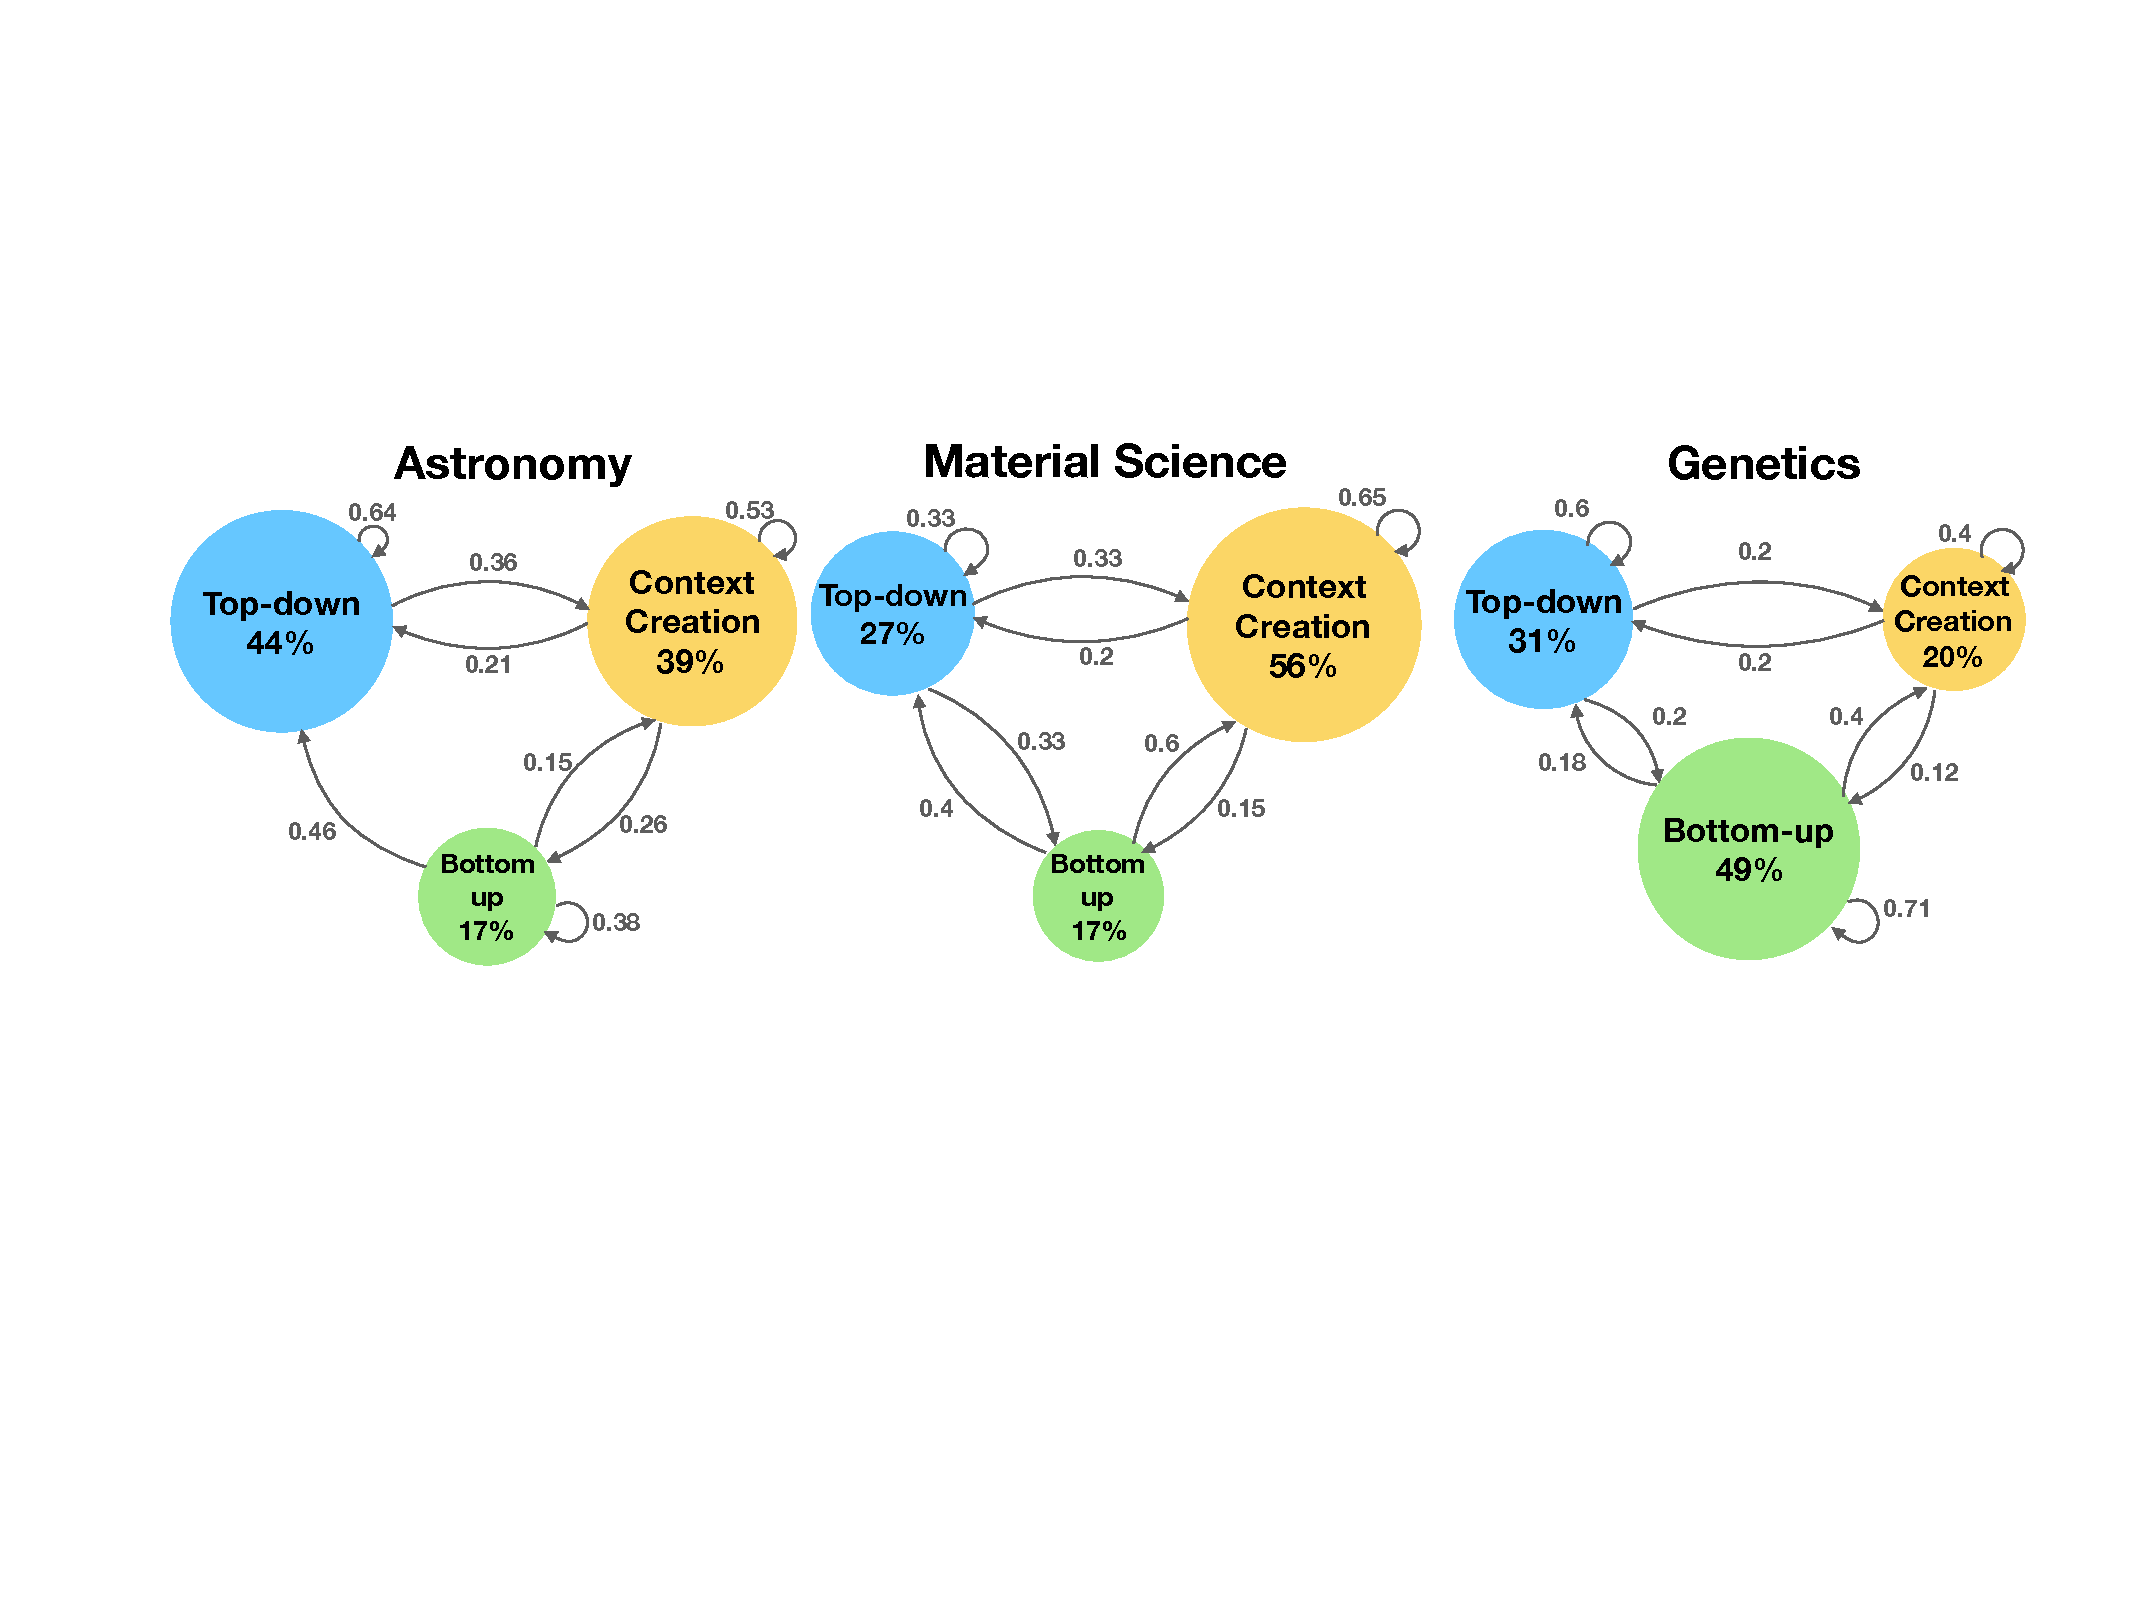
\includegraphics[width=\linewidth]{figures/markov_transition.pdf}
 %   \caption{Markov models computed based on evaluation study event sequences, with edges denoting the probability that participant in the particular domain will go from one sensemaking process to the next. Nodes are scaled according to the eigenvector centrality, representing the percentage of time participants would spend in a particular sensemaking process in steady state.\label{fig:transition
 %   \vspace*{-5pt}
 % \end{figure}
 % Similar to the sensemaking model proposed by Pirolli and Card~\cite{Pirolli}, the ---- sensemaking loop representing iterative process
 % ---- highlights how the two newly discovered VQS sensemaking process in this paper are essential for `closing the loop' between the sensemaking acts in VQSs. %, equally important
 % both the browsing-act through recommendations and performing search via these results are
 %These examples show that both the browsing-act through recommendations and performing search via these results are
 %The three sensemaking ----- not mutually exclusive, participants can go from one to the next and there is no single progression (e.g. context --> bottom -up --> top-down). Iterative blah blah. three process are equally important.
 %The three paradigms of sensemaking described earlier are not mutually exclusive.
 %Different sensemaking processes can be useful for different problem contexts.
 \par To study how important each sensemaking process
 is for participant's overall analysis,
 we compute the eigenvector centrality of each graph,
 displayed as node labels in Figure~\ref{fig:transition}.
 These values represent the percentage of time the participants
 spend in each of the sensemaking processes
 when the transition model has evolved to a steady state~\cite{pierre2011}.
 Given that nodes in Figure~\ref{fig:transition}
 are scaled by this value, in all domains,
 we observe that there is always a prominent node
 connected to two less prominent ones---but it is also clear
 that all three nodes are essential to all domains.
 Our observation demonstrates how \emph{participants
 often construct a central workflow
 around a main sensemaking process \change{based on their analytical \textbf{goals}
 and interleave variations with the two other \textbf{support} processes as they iterate on the analytic task}}, as illustrated in Table~\ref{science_task}. For example, \change{the} material scientists focus on context creation 56\% of the time, mainly through dynamic class creation,
 followed by bottom-up inquiries (such as drag-and-drop)
  and top-down pattern searches (such as sketch modification).
 %through dynamic classes than top-down pattern search. %astronomers focus largely on performing top-down pattern search, while filtering on the visualization space. %in Section~\ref{sec:pd_findings}}.
 The central process adopted by each domain
 is tightly coupled with the problem characteristics associated with each domain. For example, without an initial query in mind,
 geneticists relied heavily on bottom-up querying
 through recommendations to jumpstart their queries.
 %Despite the differing levels of usage from each subject area, we learn that \textit{each sensemaking process fulfills a central role in participants' analysis to address their high-level research objectives}.
 % \agp{maybe point to figure?}.
 % they brought to the study
 %pattern instance and visualized attributes
 \par The Markov transition model exemplifies how participants
 adopted a diverse set of workflows
 based on their unique set of research questions. The bi-directional and cyclical nature
 of the transition graphs in Figure~\ref{fig:transition} highlight how the three sensemaking processes do not simply follow a linear progression towards finding a single pattern or attribute of interest. %, going from unknown to known in the Figure~\ref{2dmodel problem space}
 Instead, the high connectivity of the transition model illustrates how these three equally-important processes form a sensemaking loop, representing iterative acts of dynamic foraging and hypothesis generation. \change{This finding reinforces the importance of each sensemaking process and indicates that future VQSs need to be \emph{integrative} in supporting all three sensemaking process to enable a diverse set of potential workflows for addressing a wide range of analytical inquiries.} %This flexibility is enabled by the diverse set of potential workflows that could be constructed in an integrative VQS like \zvpp, for addressing a wide range of analytical inquiries.%single-directional%. The VQS sensemaking loop%full-fledged
 \begin{table}[h!]
   \centering
   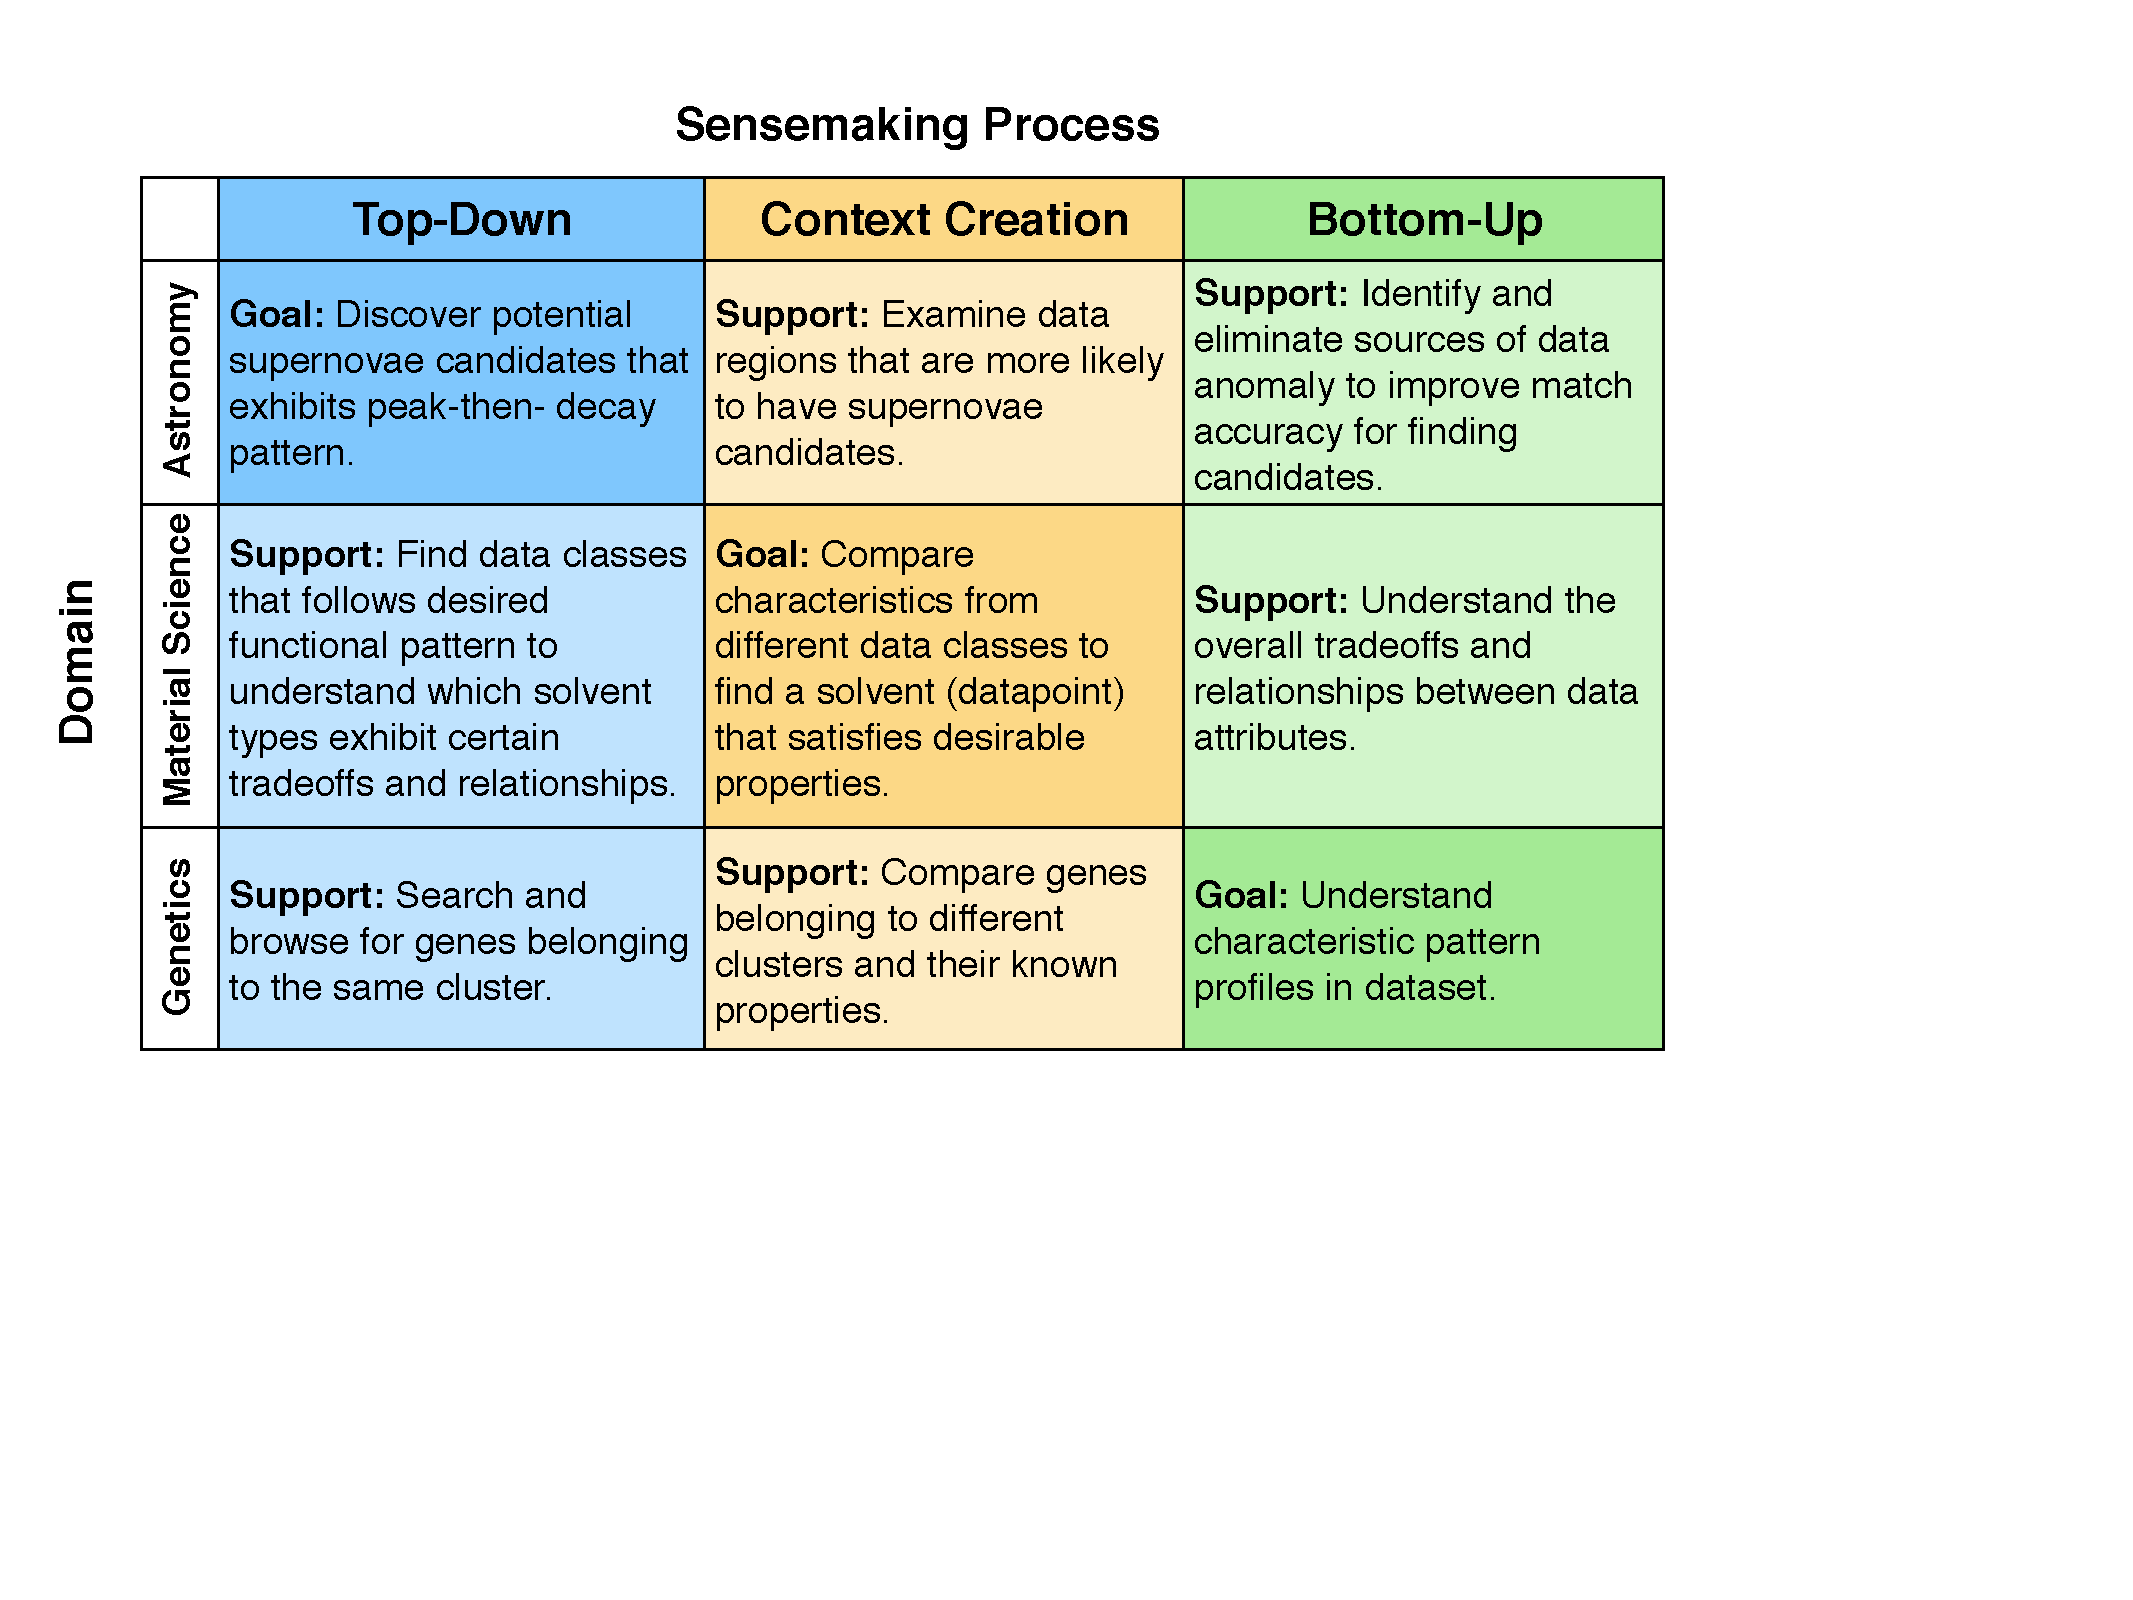
\includegraphics[width=\linewidth]{figures/science_task.pdf}
   \vspace{-6pt}\caption{\change{Each VQS sensemaking process maps to scientific tasks and goals from each use case, from pattern search to comparing visualization collections to \achange{improving} overall data understanding. We find that our participants typically have one focused goal expressible through a single sensemaking process, but since their desired insights may not always be achievable with a single \achange{class of} operation, they make use of the two other sensemaking processes to support them in accomplishing their main goal.}}
   \label{science_task}
   \vspace{-10pt}
\end{table}
 \subsection{Limitations}%suggests that direct sketch is inefficient
 \par Although evidence from our evaluation study \change{points to the infrequent use of direct sketch}, we have not performed controlled studies with a sketch-only system as a baseline to validate this hypothesis. The goal of our study is to uncover qualitative insights that might reveal why VQSs are not widely used in practice; further validation of specific findings is out of the scope of this paper. \change{While concerns regarding study results being focused on \zvpp must be acknowledged, we note that \zvpp is one of the most comprehensive VQSs to-date, covering many of the features from past systems and more (as evident from Table 1). We believe that our integrative VQS, \zvpp, can serve as a baseline for future research in VQS to evaluate against and build upon.} Given that this paper covered three design studies along with one evaluation study, we were unable to cover each domain to the level of detail typically found in a dedicated design study paper. Instead, our focus was to highlight the differences and similarities among these domains relevant to the capabilities required in VQS and we defer domain-specific participatory design details and artifacts to Appendix~\ref{apdx:pdartifact}. \achange{Future longitudinal studies may also help alleviate the novelty effects that participants may have experienced during the evaluation study.} While we have generalized our findings \change{beyond existing work} by employing three different and diverse domains (see Figure~\ref{fig:transition}),
 our case studies have so far
 been focused on scientific data analysis \change{with domain-experts},
 as a first step towards greater adoption of VQSs.
 Other potential domains that could benefit from VQSs include:
 financial data for business intelligence,
 electronic medical records for healthcare,
 and personal data for ``Quantified Self''.
 These different domains may each pose different sets of challenges \change{(such as designing for novices as end-users)} unaddressed by the findings in this paper,
  pointing to a promising direction for future work.
%!TEX root = main.tex
 \section{Conclusion\label{sec:conclusion}}
 While VQSs hold tremendous promise in accelerating data exploration, they are rarely used in practice. We worked closely with analysts from three diverse domains to characterize how VQSs can address their analytic challenges, collaboratively design VQS capabilities, and evaluate how VQSs are used in practice. Participants were able to use our final system, \zvpp, for discovering desired patterns, trends, and valuable insights to address unanswered research questions. Based on these experiences, we developed a sensemaking model for how analysts make use of VQSs. Contrary to past work, we found that sketch-to-query is not as effective in practice as past work may suggest. Beyond sketching, we find that each sensemaking process fulfills a central role in participants' analysis workflows to address their high-level research objectives. We advocate that future VQSs should invest in understanding and supporting all three sensemaking processes to effectively ``close the loop'' in how analysts interact and perform sensemaking with VQSs. 
 \cut{While more work certainly remains to be done, by contributing to a better understanding of how VQSs are used in practice across domains, our paper can serve as a roadmap towards the broader adoption of VQSs for novel future use cases.}
 %can also serve as a roadmap for broader adoption of VQSs,and hopefully trigger exploration of novel use cases for these tools
 % the application of VQSs to ---- opportunities beyond ----
 % for the broad adoption of VQSs in data analysis, opening up potential unexplored use cases and opprtunity for VQS. envision opportunities for VQSs beyond this to a larger space of use cases.
 % process In discovering two ----- en ---opening up pathways  potential pathway worflow, while clo---- .
 % learn about the challenges they face when working with data. We extended our VQS \zv to the point where it could be effectively used for scientific data analysis.
 % Through participatory design, we identified three classes of missing interface capabilities  essential for employing VQSs for facilitating insight in real scientific applications, spanning expressive querying and dynamic faceting, as well as fine-grained control and understanding, along with the ability to compose flexible workflows in an integrated manner (RQ2). Finally, our evaluation study demonstrated how these features helped accelerate scientific insights (RQ3), as well as how they fit in the context of data analysis workflows (RQ4). One such finding is that bottom-up querying (e.g., drag-and-drop) is preferred over top-down (e.g., sketching) for exploratory data analysis, contrary to what is commonly supported in existing VQSs.
 % point to focus on sci data but future work on quantified self and social viz
 % VQS important
 % Our work :
 % - \zvpp
 % - sensemaking model
 % domain problem characterization of visual querying through design studies with three different subject areas,
 % \item abstraction of taxonomy and design space of VQSs grounded in participatory design findings,
 % \item a full-fledge VQS, \zvpp, capable of facilitating rapid hypothesis generation and insight discovery,
 % \item evaluation study findings regarding how VQSs are used in practice, leading to the formation of a novel sensemaking model for VQSs. %including the ineffectiveness of sketching and the ---- workflow
 % discover sketch
 % Our work closes the loop in VQS sensemaking so that VQS works in scenarios  where XY is unknown or Z is unknown. These areas were previously unexplored by past works.
 % As presented in this section, our study is the first that contributes towards a holistic understanding of the sensemaking process for visual querying.
 % ----- how they are used in practice. %Rather than assuming visual querying through sketch is useful, we
 % Our work is the first that evaluate on multiple case study participatory design, longitudinal study.
 % Participants intermixed functionalities across different sensemaking paradigms to address their problem contexts.
  % more thoroughly characterize the problem design space of VQSs and taxonomy abstraction for understanding the sensemaking process in VQSs. Moreover, we performed design studies with three different subject areas with a diverse set of questions, datasets, and challenges to further generalize our findings.
  % facilitating a diverse set of potential workflows and
  % Both query by sketch and equations adopt a problematic assumption that analysts start with a known and easy-to-specify search pattern in mind.
 
\newpage
\bibliographystyle{abbrv-doi}
\bibliography{reference}
\clearpage
% \vspace*{-15pt}
\onecolumn
 \appendix
 % \vspace*{-15pt}
 % \npar\textbf{{\huge Appendix}}
 \npar In Appendix A, we first describe additional details about the participatory design process, as well as domain-specific artifacts collected from contextual inquiry. Next, in Appendix B, we articulate the space of problems amenable to VQSs and describe how the sensemaking processes (introduced in Section~\ref{sec:sensemaking}) fit into different parts of the problem space. In Appendix C, we provide supplementary information regarding our analysis methods and results for the evaluation study. In Appendix D, we acknowledge the individuals and agencies that have made this work possible. 
 % \vspace*{-10pt}
 \section{Artifacts from Participatory Design\label{apdx:pdartifact}}
 % \vspace*{-10pt}
 \npar Information about each participants can be found in Table~\ref{participants}. 
  \begin{table}[h!]
  \captionsetup{font=normalsize,labelfont=normalsize}
    \centering
    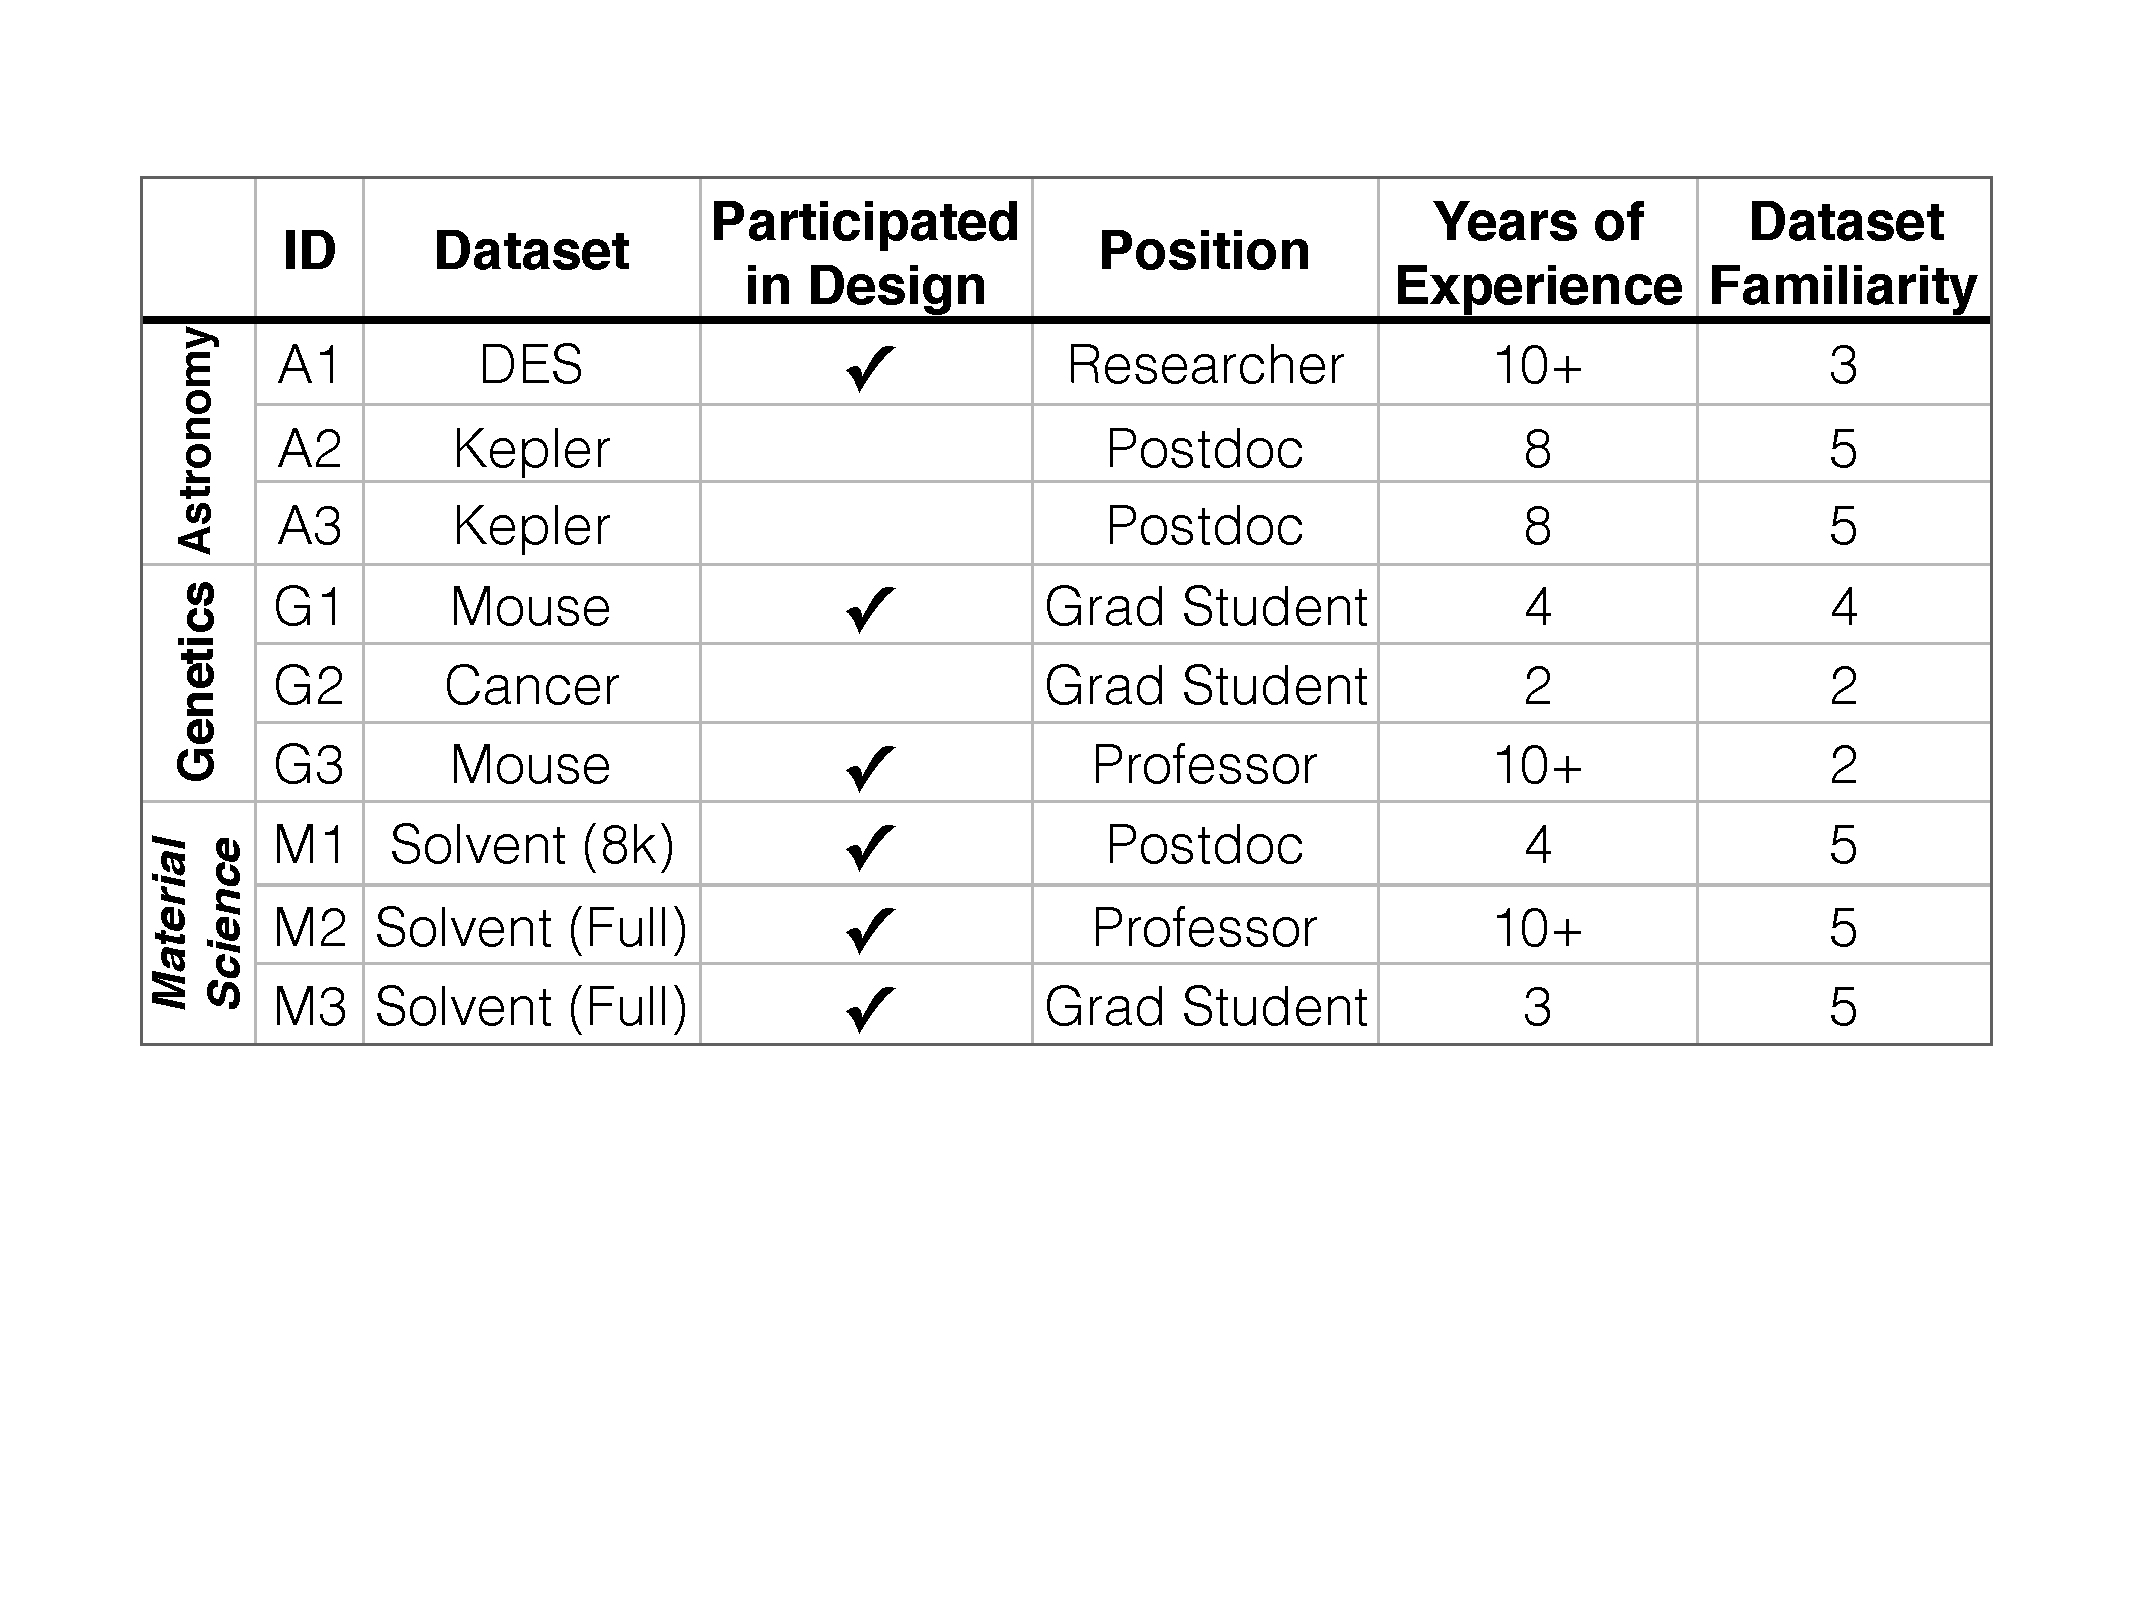
\includegraphics[width=0.5\linewidth]{figures/participant_info.pdf}
    \caption{Participant information. The Likert scale used for dataset familiarity ranges from 1 (not familiar) to 5 (extremely familiar).}
    \label{participants}
    % \vspace*{-15pt}
  \end{table}
 \npar During the contextual inquiry, participants demonstrated the use of domain-specific tools for conducting analysis in their existing workflow, including:
   \begin{denselist}
     \item \href{http://descut.cosmology.illinois.edu}{Image Cutout Service (Astronomy)}
     \item \href{http://cs.cmu.edu/~jernst/stem/}{Short Time-series Expression Miner (Genetics)}
     \item \href{http://srdata.nist.gov/solubility/}{Solubility Database (Material Science)}
   \end{denselist}
\begin{figure}[h!]
\captionsetup{font=normalsize,labelfont=normalsize}
 \centering
 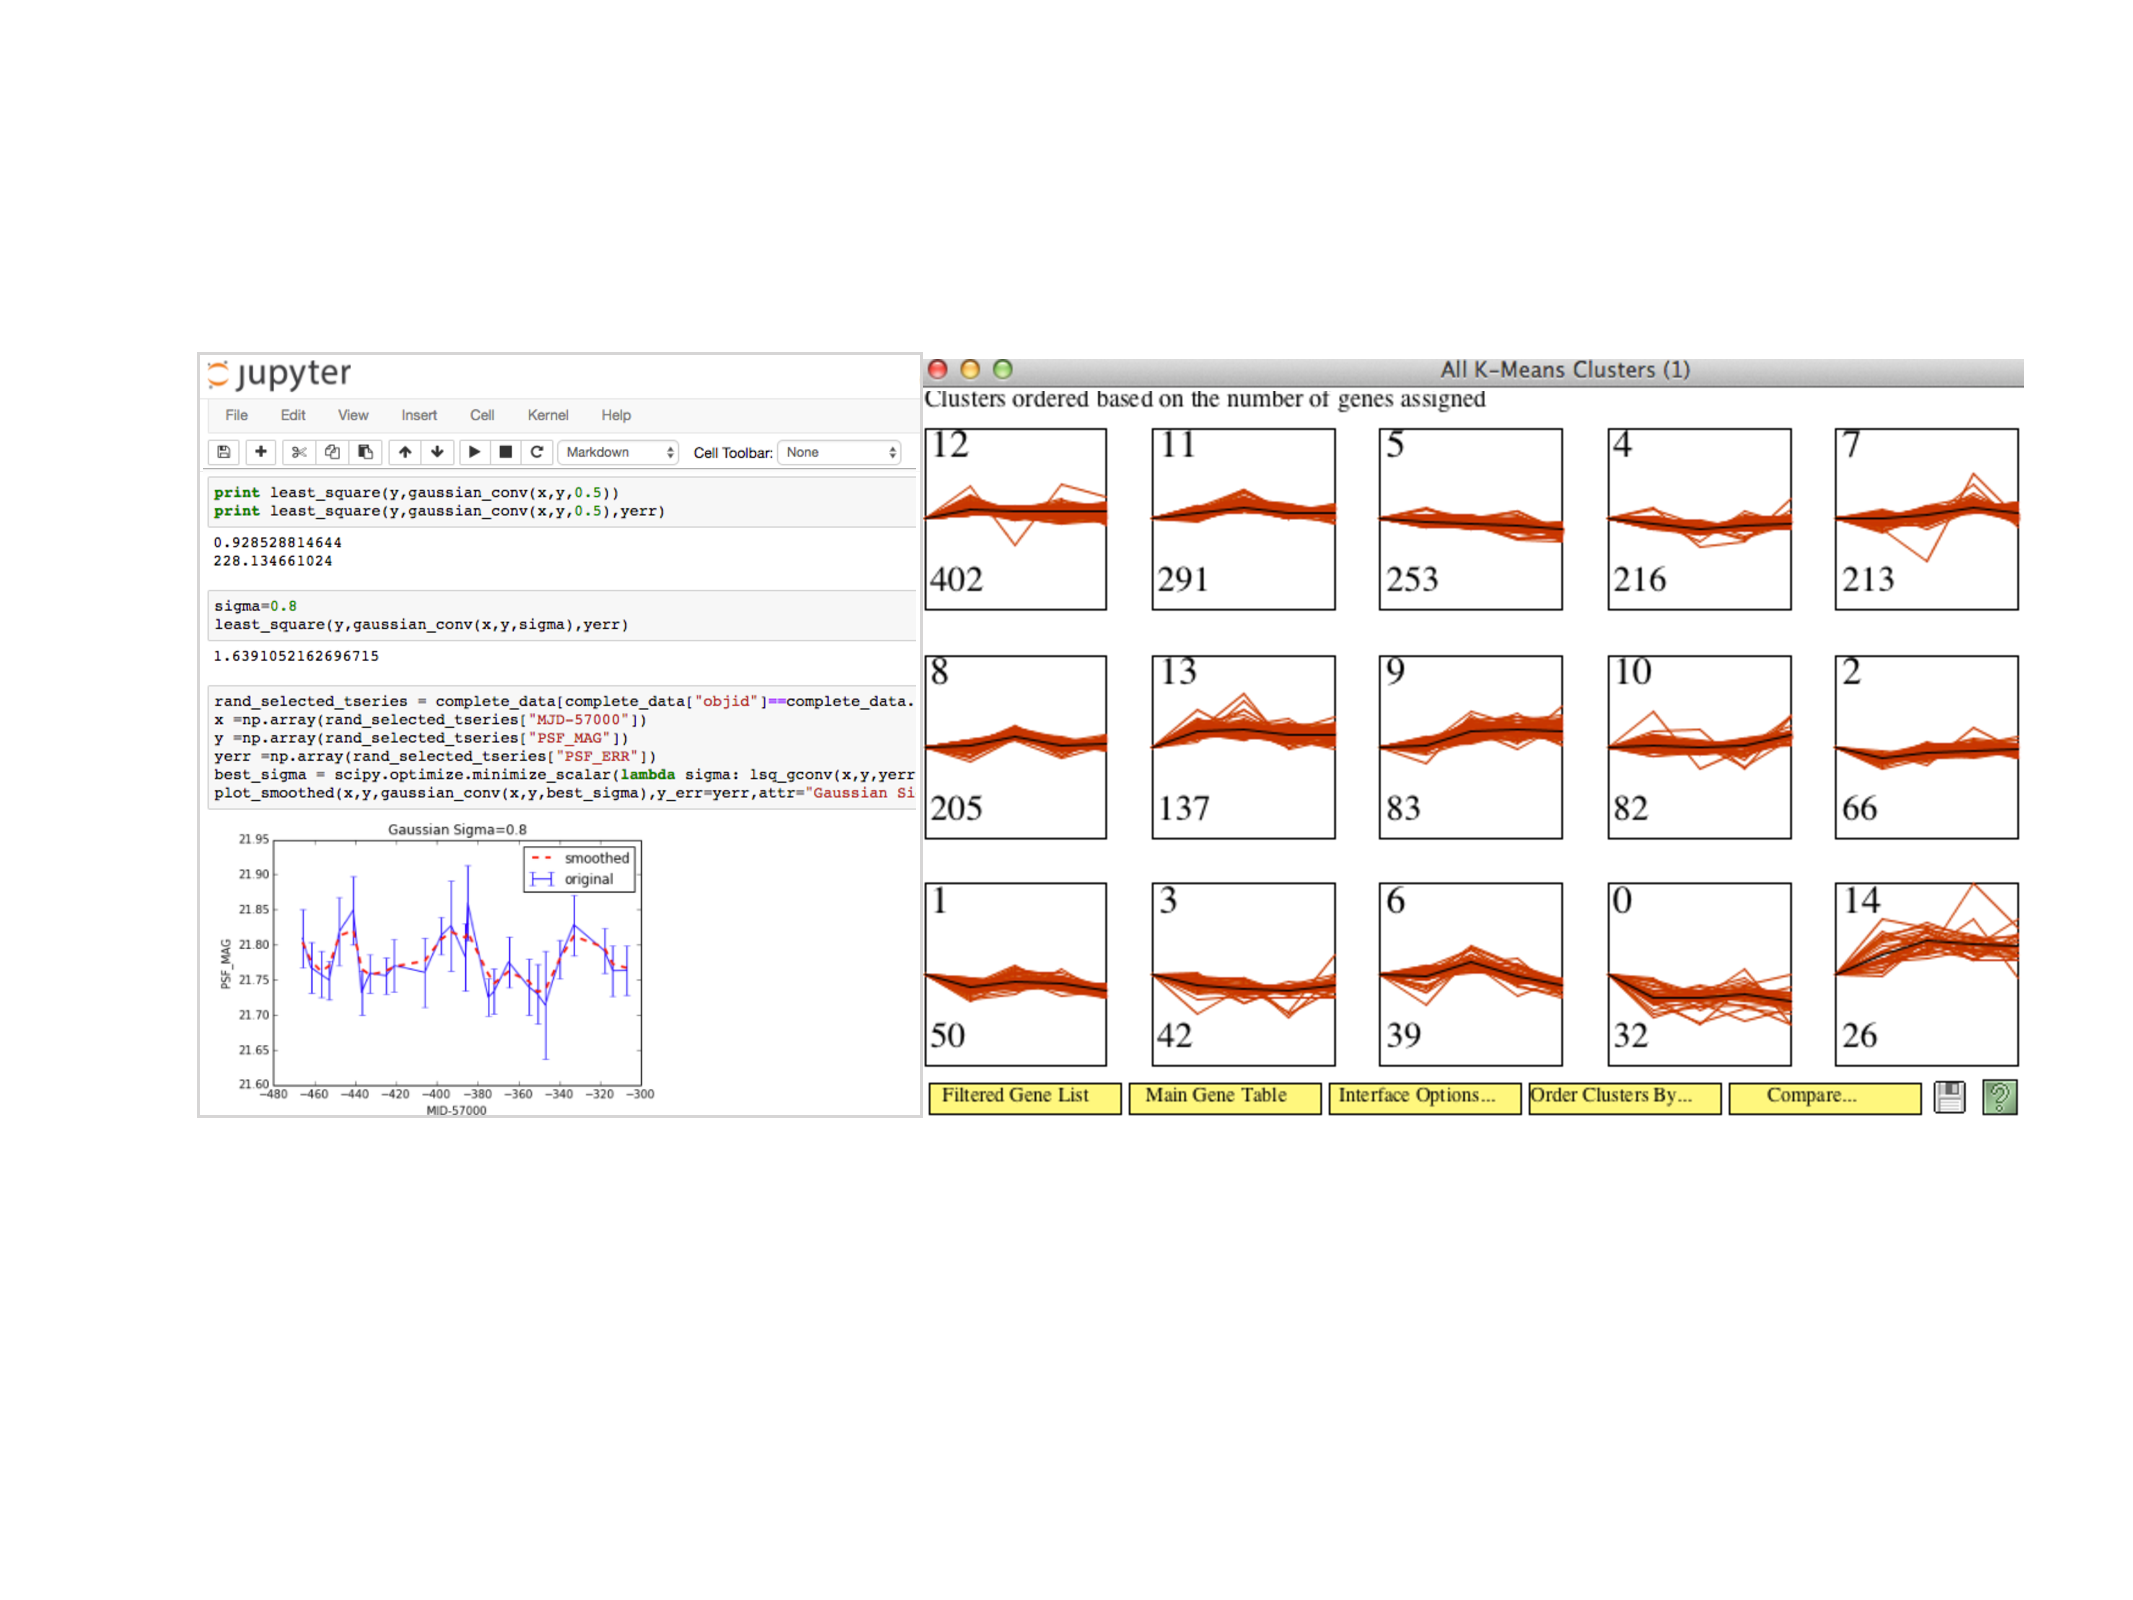
\includegraphics[width=0.8\linewidth]{figures/CIscreenshot.pdf}
 \caption{\rchange{Screenshots from contextual inquiry. Left: A1 performs data smoothing to clean the data and then examines a light curve manually using a Jupyter notebook. Right: G2 uses a domain-specific software to perform clustering and visualize the outputs.}}
 \label{CIscreenshot}
 % \vspace*{-15pt}
\end{figure}
\begin{figure}[h!]
  \captionsetup{font=normalsize,labelfont=normalsize}
    \centering
    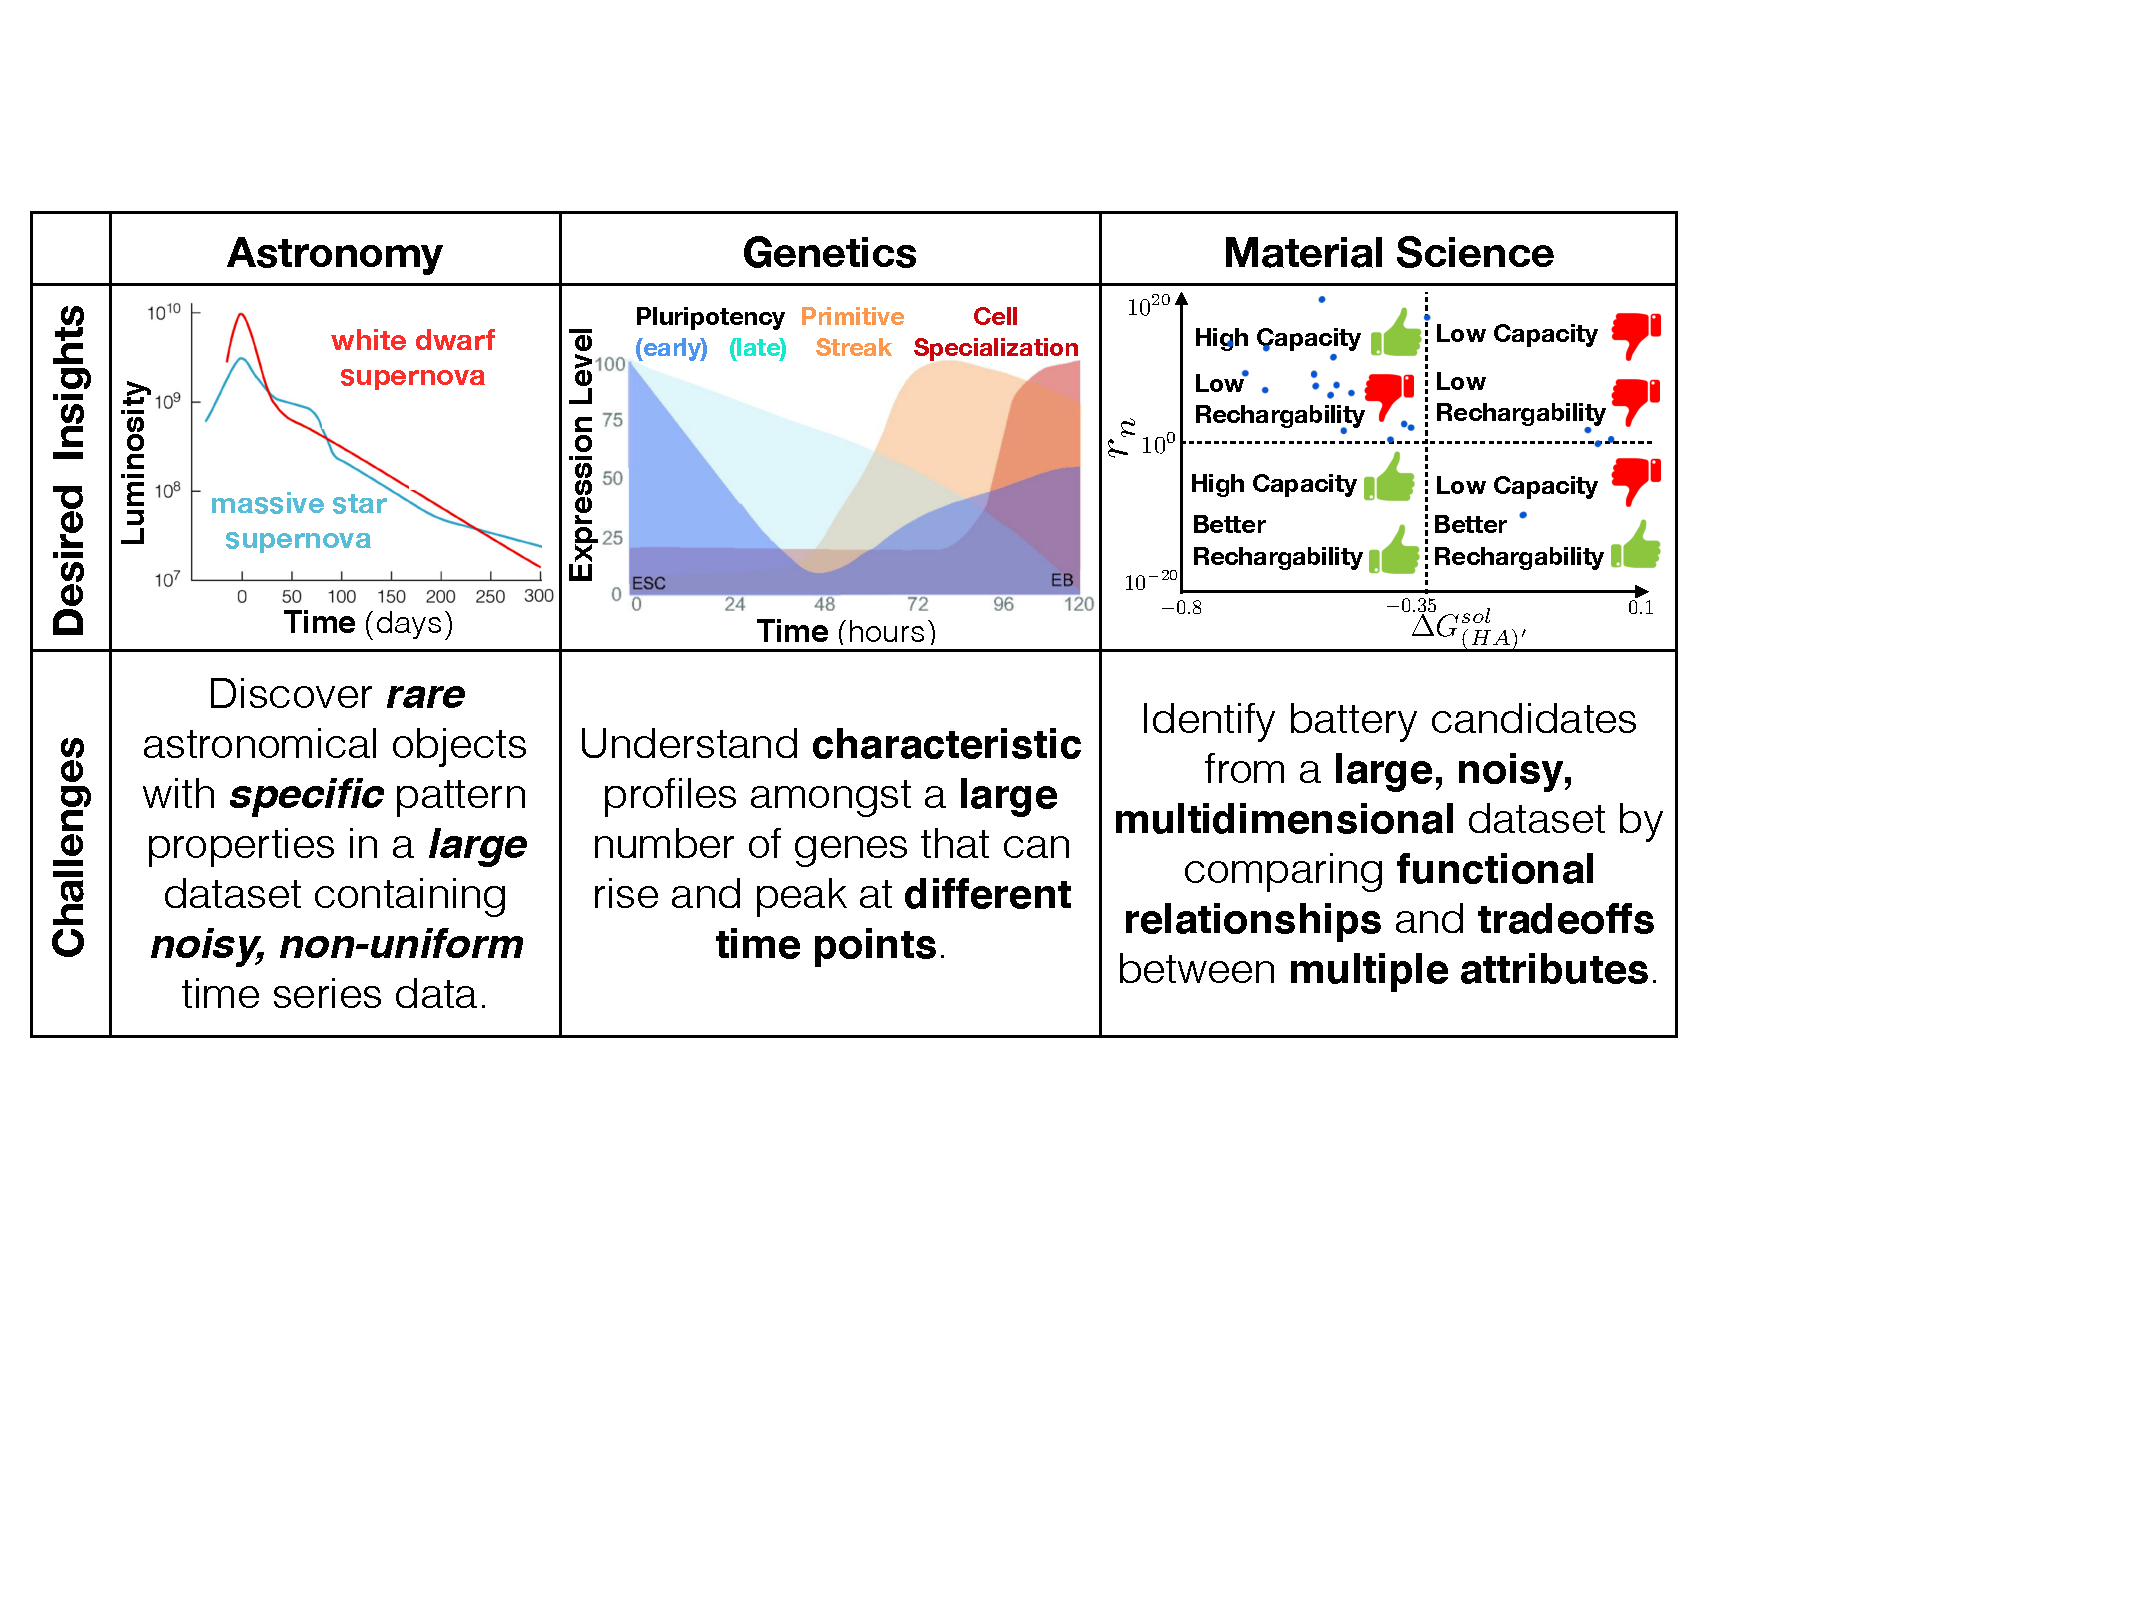
\includegraphics[width=0.5\linewidth]{figures/science_goal.pdf}
    \caption{Desired insights, problem and dataset challenges for each of the three application domains in our study.}
    \label{science_goal}
    % \vspace*{-15pt}
   \end{figure}
 \newpage
 \npar Our collaboration with participants is illustrated in Figure~\ref{timeline}, where we began with an existing VQS (\zv, as illustrated in Figure~\ref{oldZV}) and incrementally incorporated features, such as dynamic class creation (Figure~\ref{dcc}), throughout the PD process. 
 \begin{figure}[h!]
 \captionsetup{font=normalsize,labelfont=normalsize}
 	\centering
 	% \captionsetup{justification=centering,margin=2cm}
 	% 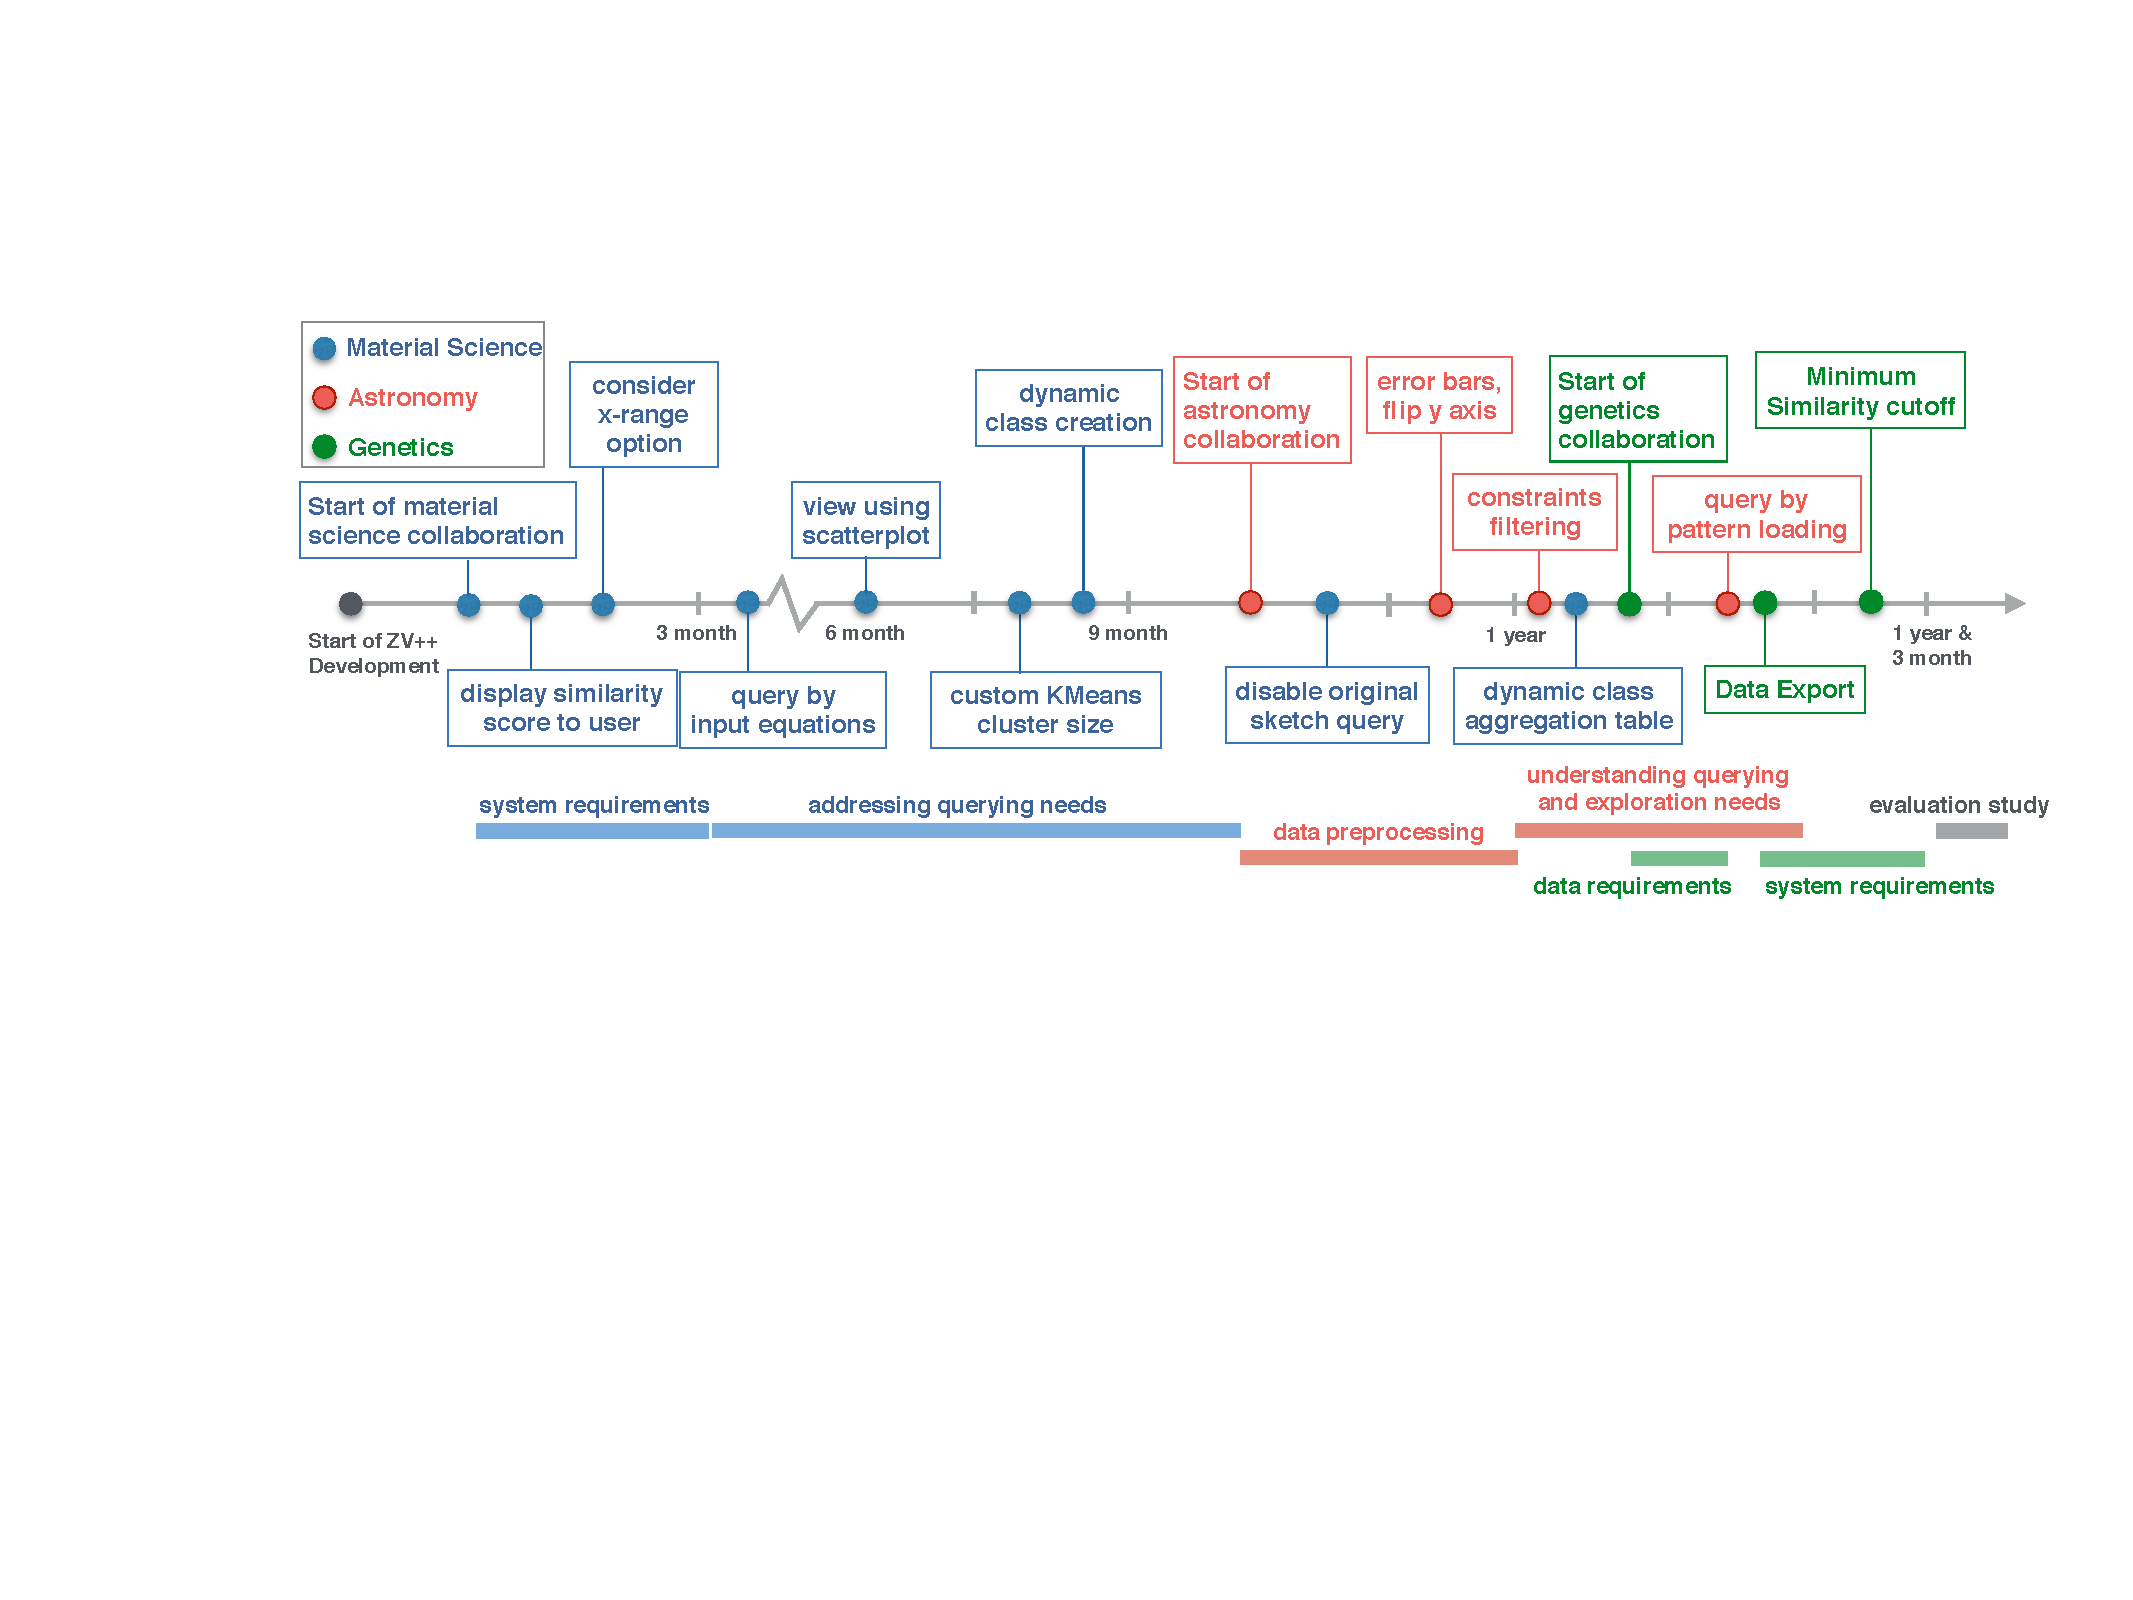
\includegraphics[width=6in]{figures/timeline.pdf}
   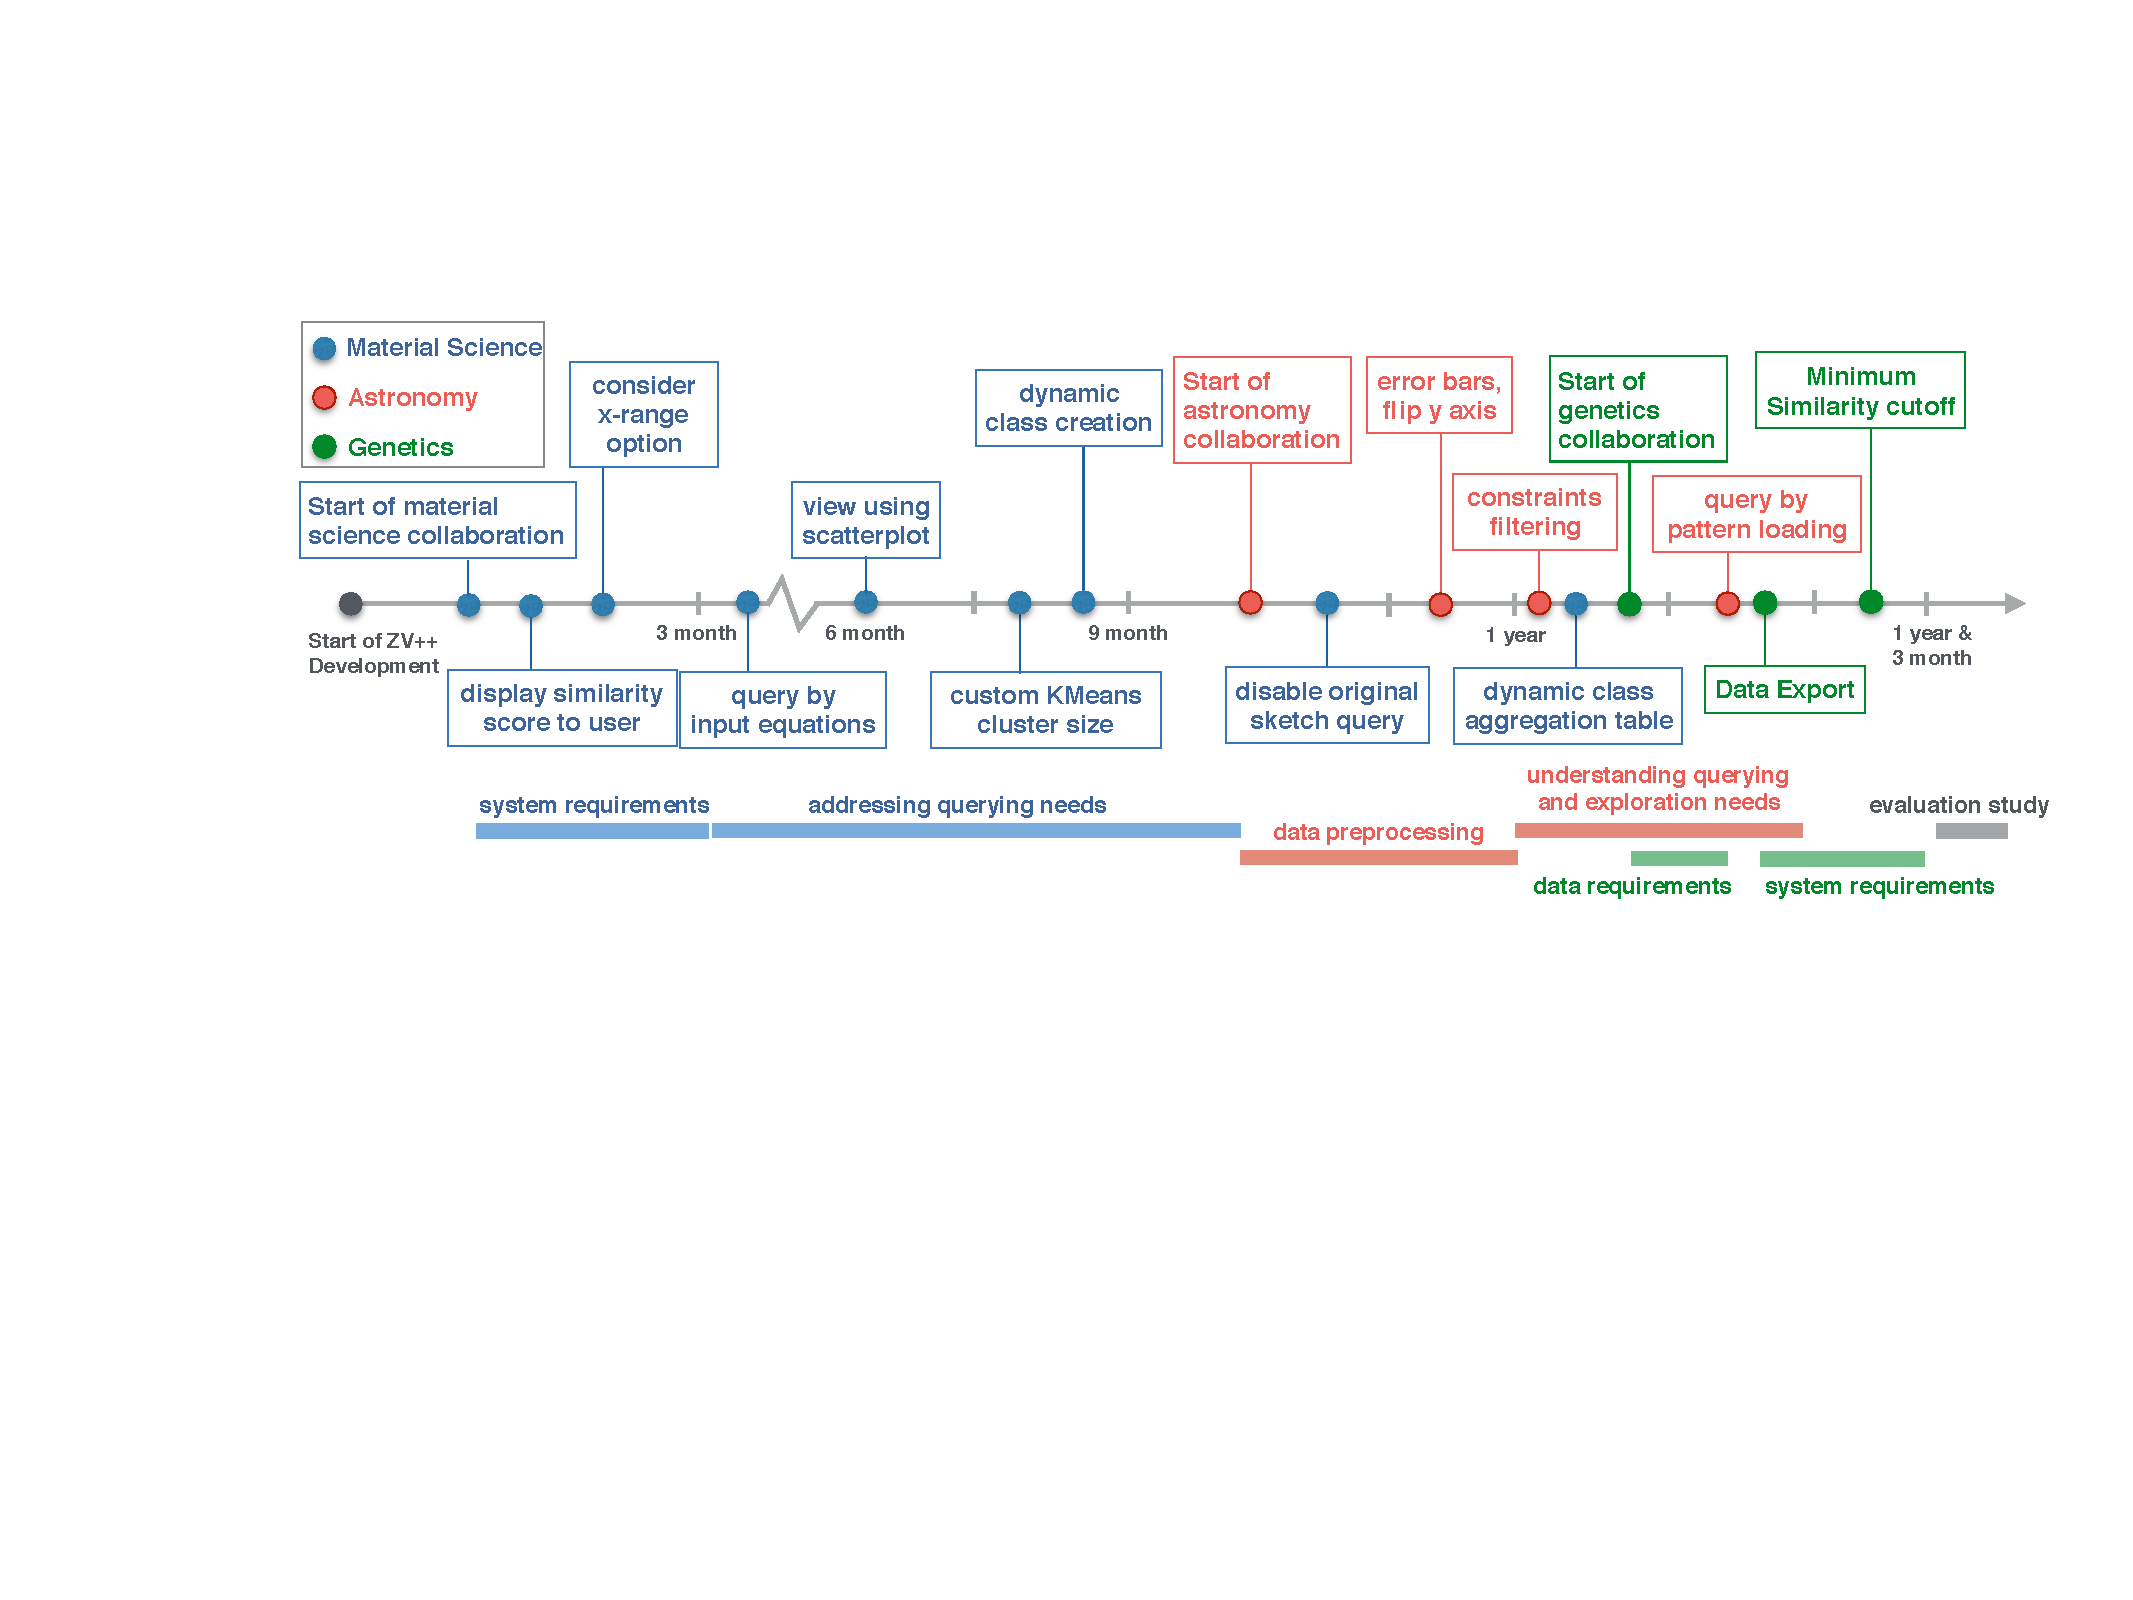
\includegraphics[width=0.8\linewidth]{figures/timeline.pdf}
 	\caption{Timeline for progress in participatory design studies.}
 	\label{timeline}
 	% \vspace{-10pt}
 \end{figure}
 \begin{figure}[h!]
 \captionsetup{font=normalsize,labelfont=normalsize}
 	\centering
 	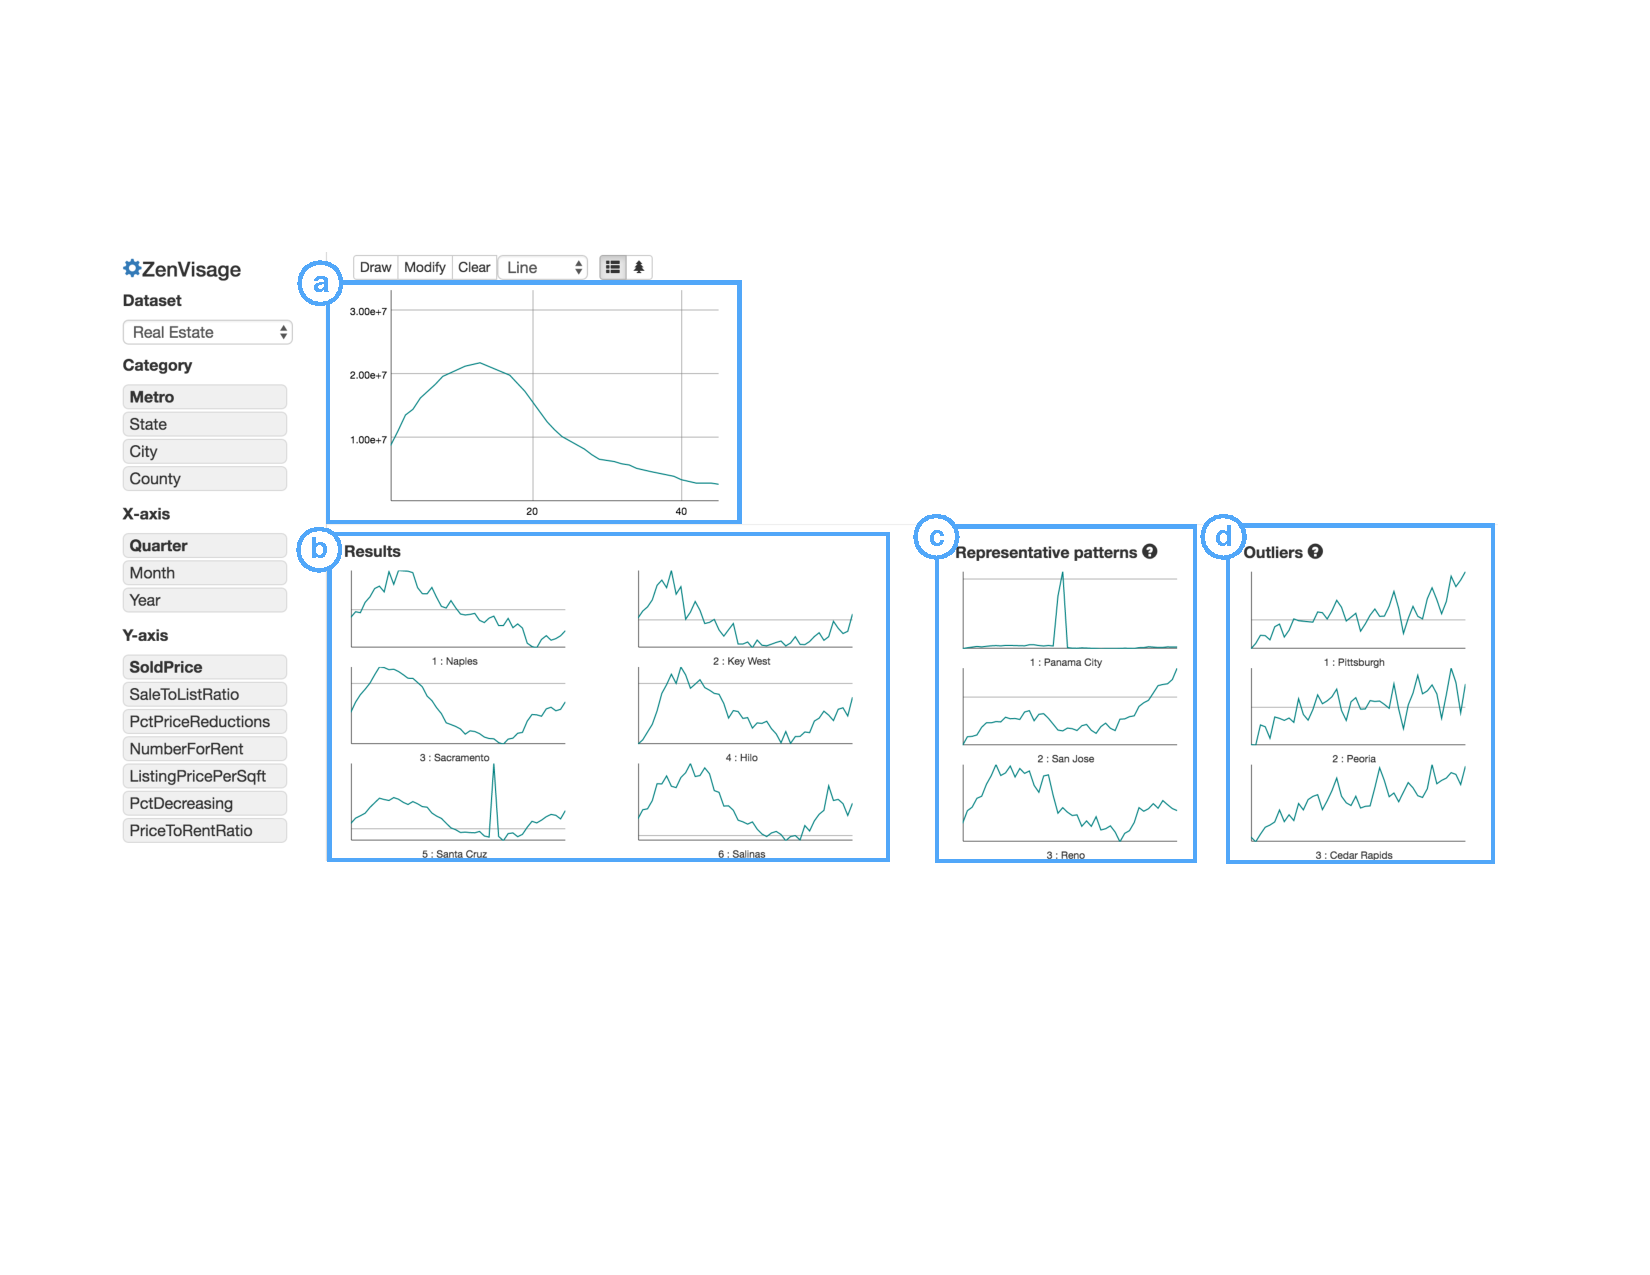
\includegraphics[width=0.85\linewidth]{figures/oldZV_nozql.pdf}
 	\caption{The existing \zv prototype allowed users to sketch a pattern in (a), which would then return (b) results that had the closest Euclidean distance from the sketched pattern. The system also displays (c) representative patterns obtained through K-Means clustering and (d) outlier patterns to help the users gain an overview of the dataset.}
 	\label{oldZV}
   % \vspace{-5pt}
 \end{figure}
 % \npar As discussed in Section~\ref{sec:feature_dsicovery}, not all of the features proposed by participants during PD were incorporated in the \zvpp prototype. Based on our meeting logs with participants, we found that reasons for not carrying a feature from the design to implementation stage included:
 % \begin{denselist} %he amount of nice-to-have features that one could envision for the tool is endless.
 % \item Nice-to-haves: One of the most common reasons for unincorporated features comes from participant's requests for nice-to-have features. To this end, we use two criteria to heuristically judge whether to implement a particular feature:
 % \begin{enumerate}[leftmargin=*]
 % \item \textit{Necessity:} Without this feature, can participants still work with this dataset using the tool and meet their information needs?
 % \item \textit{Generality:} Will this feature benefit only this specific use case or be potentially useful for other domains as well?
 % \end{enumerate}
 % \item ``One-shot'' operations: We decided not to include features that only needed to be performed once and remain fixed thereafter in the analysis workflow. For example, certain preprocessing operations such as filtering null values only needed to be performed once with an external tool.
 % \item Substantial research or engineering effort: Some proposed features did not make sense in the context of VQS or required a completely different set of research questions. For example, the question of how to properly compute similarity between time series with non-uniform number of datapoints arose in the astronomy and genetics use case, but requires the development of a novel distance metric and algorithm that is out of the scope of our design study objective. %. For example, M3 proposed functional fitting to obtain fitting coefficients. Other features
 % \item Underdeveloped ideas: Other feature requirements came from casual specification that were underspecified. For example, A1 wanted to look for objects that have deficiency in one band and high emission in another band, but the scientific definition of ``deficiency'' in terms of brightness levels was ambiguous.
 % \end{denselist}
  \begin{figure}[h!]
    \captionsetup{font=normalsize,labelfont=normalsize}
   \centering
   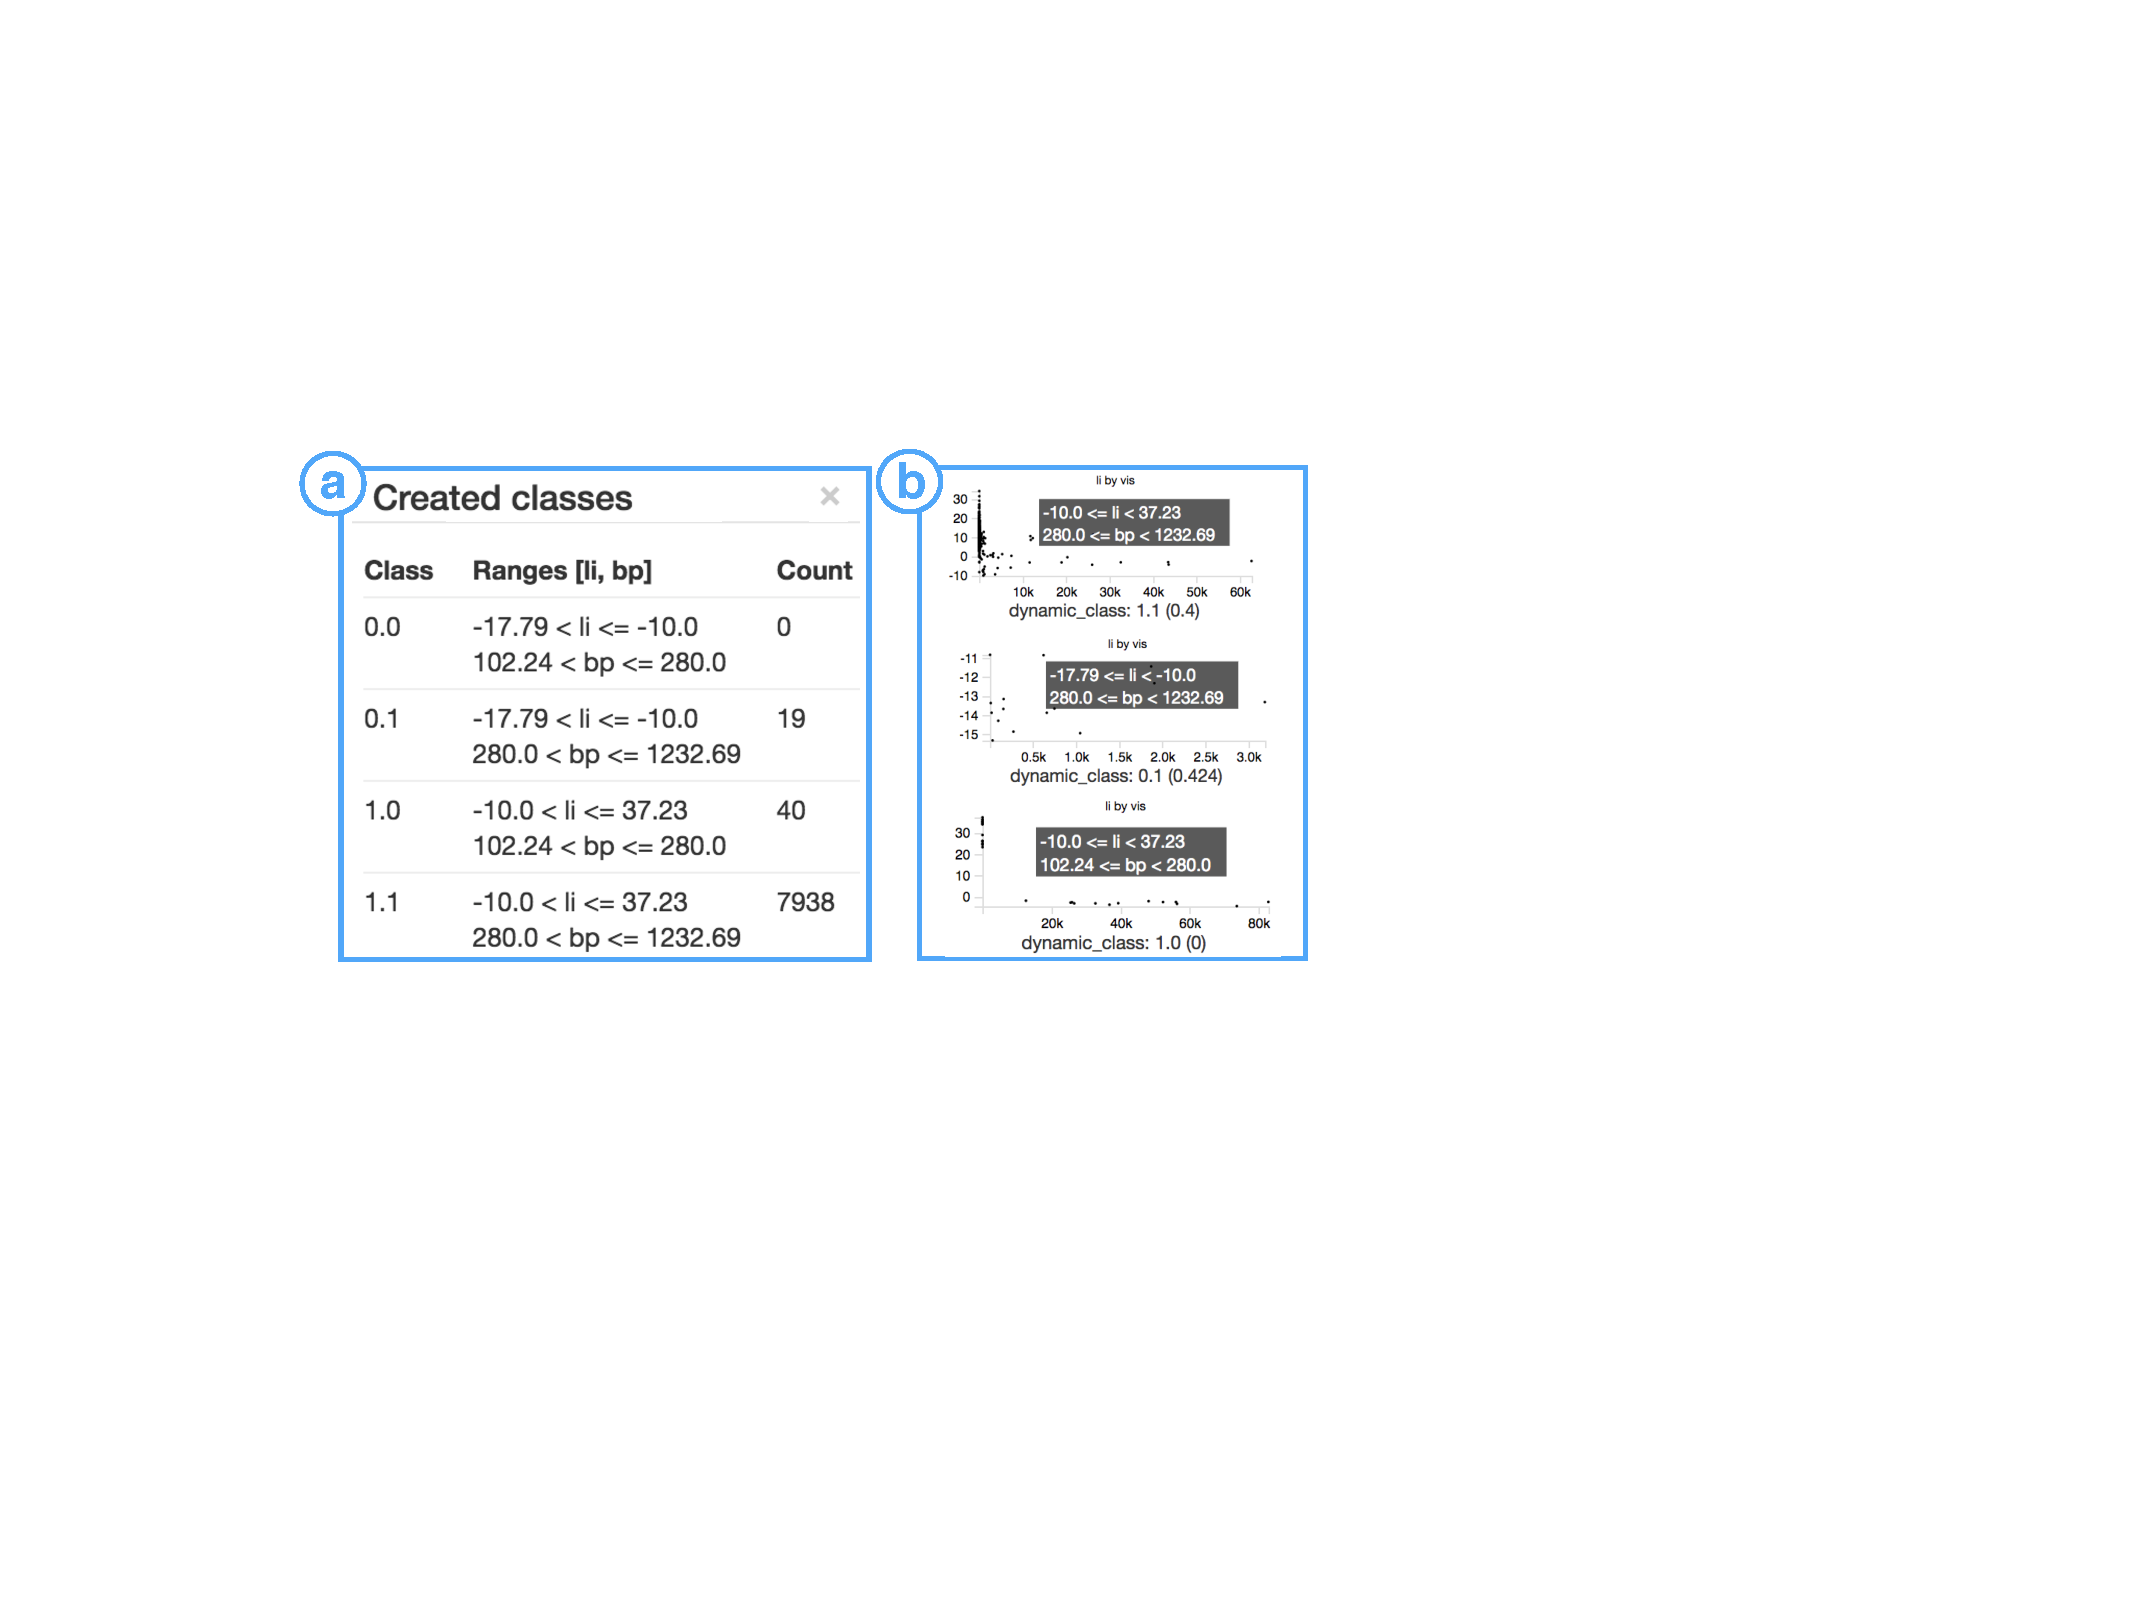
\includegraphics[width=0.55\linewidth]{figures/dcc.pdf}
   \caption{Example of dynamic classes. (a) Four different classes with different Lithium solvation energies (li) and boiling point (bp) attributes based on user-defined data ranges. (b) Users can hover over the visualizations for each dynamic class to see the corresponding attribute ranges for each class. The visualizations of dynamic classes are aggregate across all the visualizations that lie in that class based on the user-selected aggregation method.}
   \label{dcc}
   % \vspace{-10pt}
 \end{figure}
 % \newpage
 % \vspace*{-30pt}
 % \npar Table~\ref{science_task} illustrates how each of the subtasks in participant's workflow can be addressed by a sensemaking process.}
 % \begin{table}[h!]
 % 	\centering
 % 	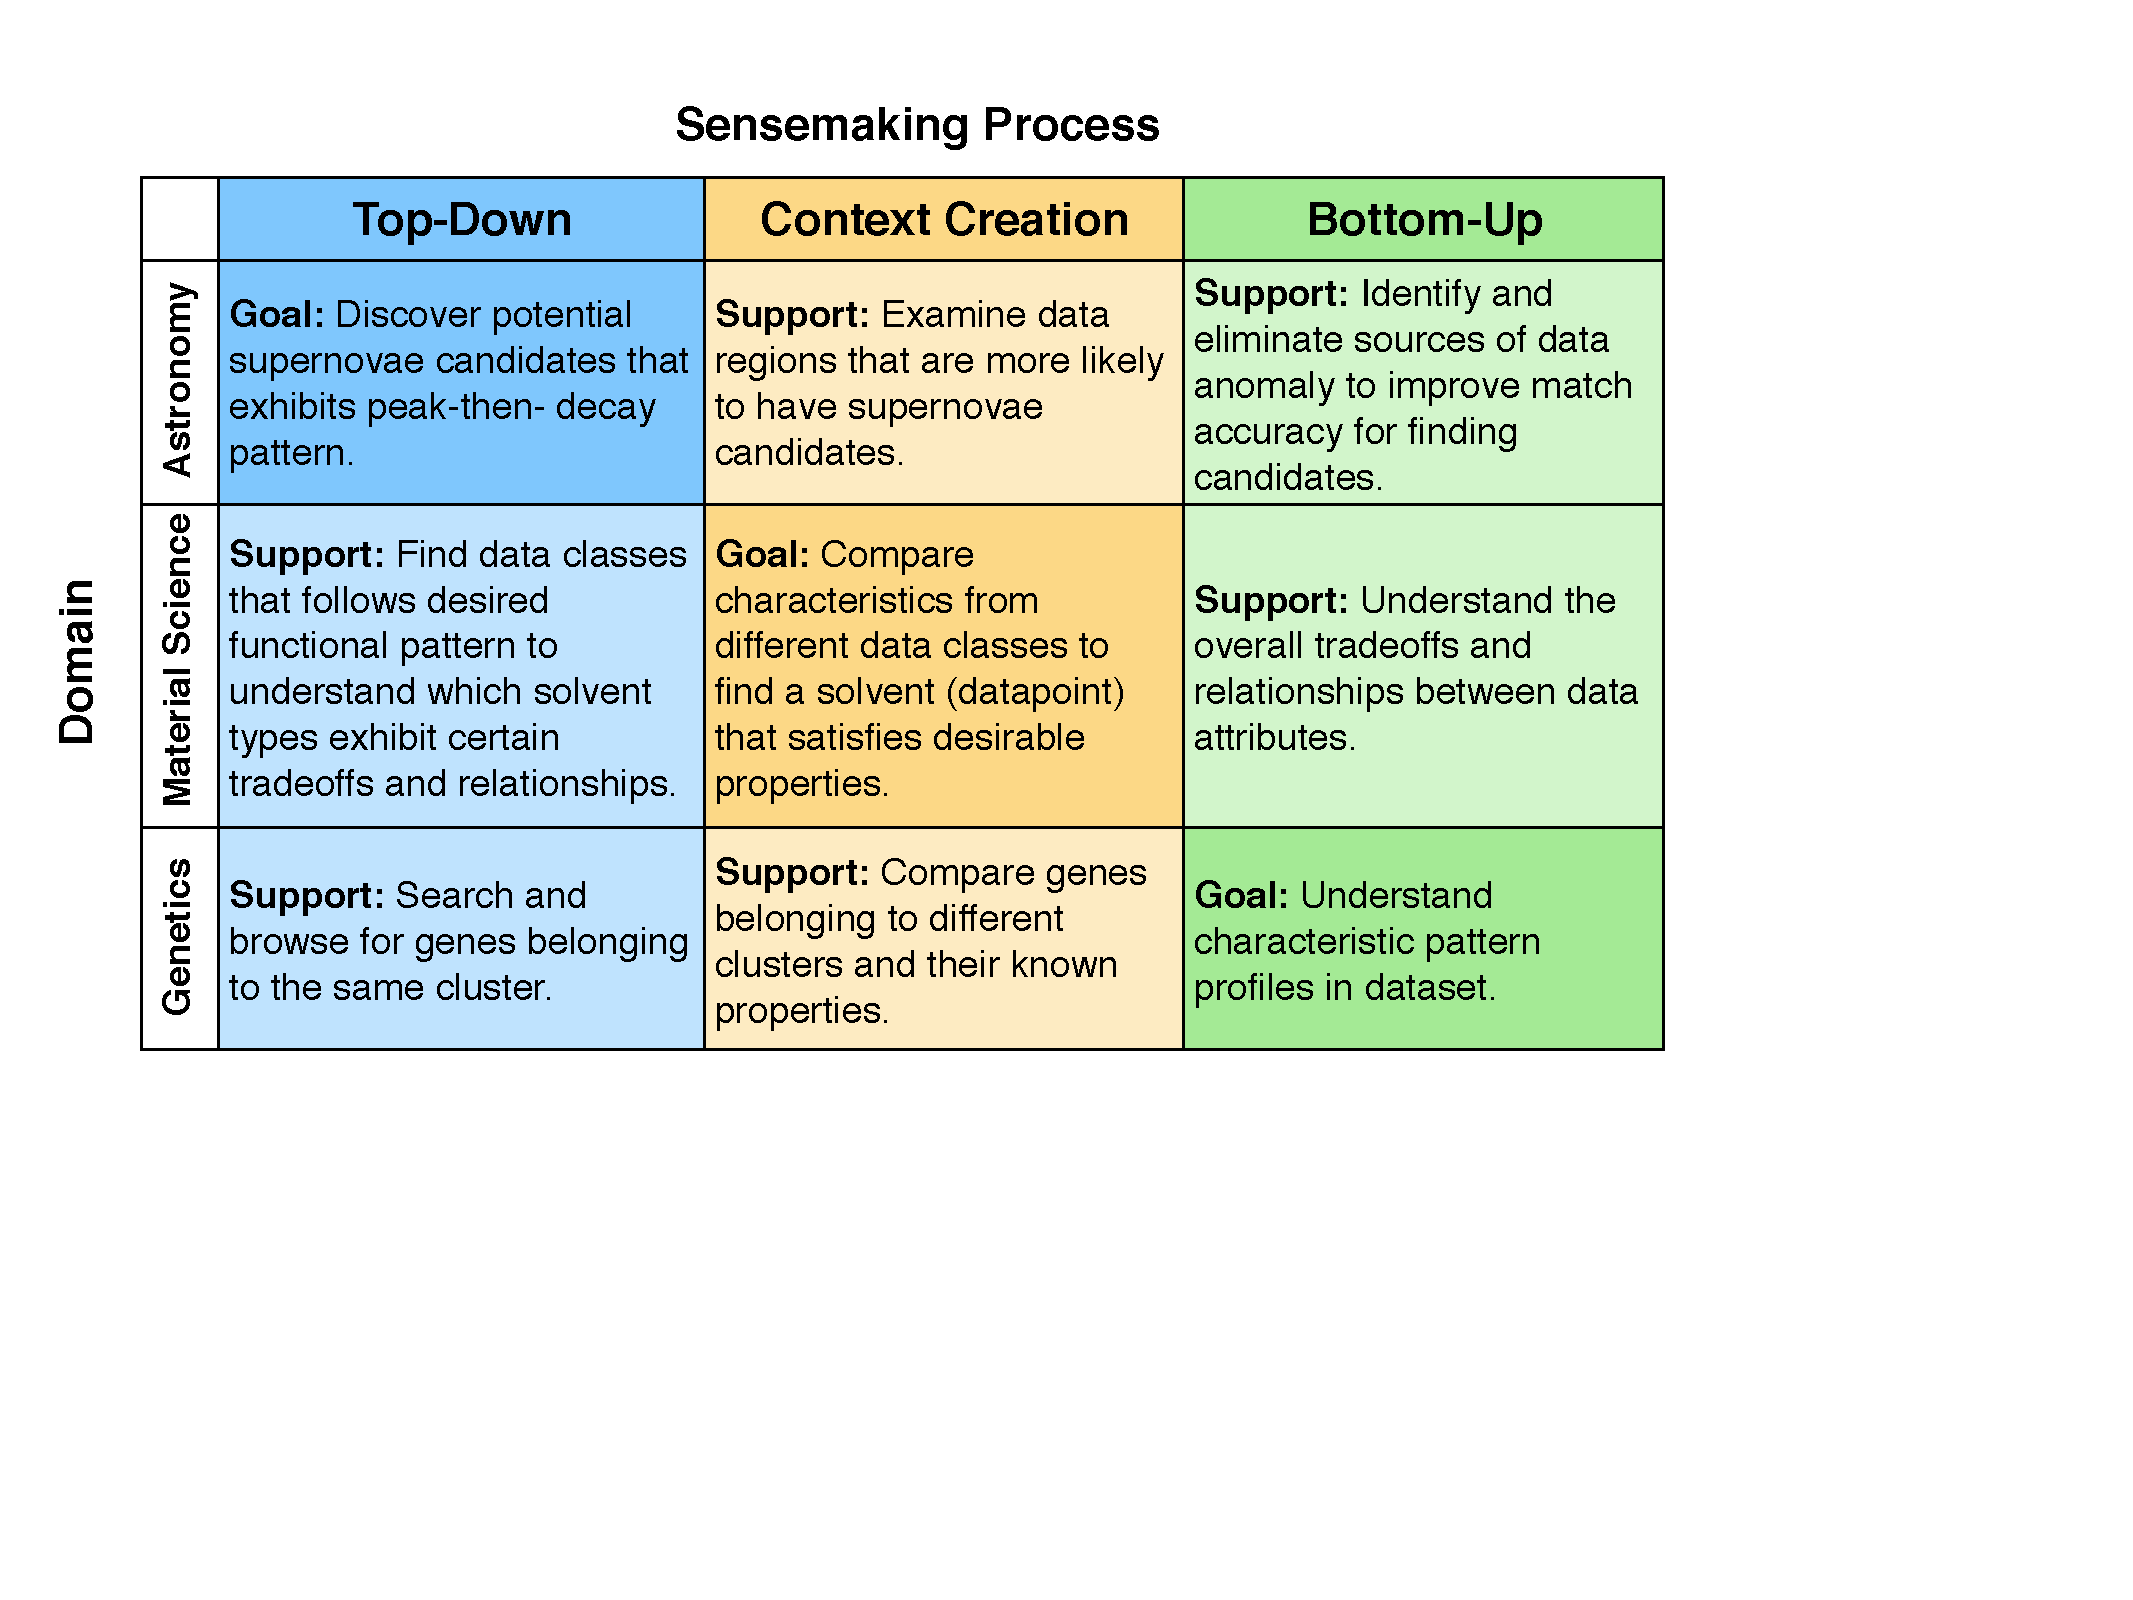
\includegraphics[width=\linewidth]{figures/science_task.pdf}
 % 	\vspace{-6pt}\caption{Each VQS sensemaking process maps to scientific tasks and goals from each use case, from pattern search to comparing visualization collections to gaining overall data understanding. We find that our scientific participants typically have one focussed goal expressible through a single sensemaking process, but since their desired insights may not always be achievable with a single operation, they make use of the two other sensemaking processes to support them in accomplishing their main goal.}
 % 	\label{science_task}
 % 	\vspace{-10pt}
 % \end{table}
 \clearpage
 \section{Characterizing the Problem Space for VQSs\label{appdx:problem_space}}
 We now characterize the space of problems addressable by VQSs and describe how each sensemaking process fits into different problem areas that VQSs are aimed to solve. Visual querying often consists of searching for a desired pattern instance (Z) across a visualization collection specified by some given attributes (X,Y). Correspondingly, we introduce two axes depicting the amount of information known about the visualized attribute and pattern instance as shown in Figure~\ref{2dmodel}.
 \npar Along the \textbf{pattern instance} axis, the visualization that contains the desired pattern may already be \texttt{known} to the analyst, exist as a pattern \texttt{in-the-head} of the analyst, or be completely \texttt{unknown} to the analyst. In the \texttt{known} pattern instance region (Figure~\ref{2dmodel} grey cell), systems such as Tableau, where analysts manually create and examine each visualization one at a time, is more well-suited than VQSs, since analysts can directly work with the selected instance without having to search for which visualization exhibits the desired pattern. We define \textit{top-down pattern search} as the process where analysts query a fixed collection of visualizations based on their in-the-head pattern (Figure~\ref{2dmodel} blue). On the other hand, \textit{bottom-up data-driven inquiries} (Figure~\ref{2dmodel} green) are driven by recommendations or queries that originate from the data (or equivalently, the visualization), since the pattern of interest is unknown and external to the user.
 %analysts often do not start with a known pattern instance. T
 \npar The second axis, \textbf{visualized attributes},
 depicts how much the analyst
 knows about which X and Y axes
 they are interested in visualizing.
 In both the astronomy and genetics use cases,
 as well as past work in this space, the attribute to be visualized is \texttt{known}, as data was in the form of a time series. In the case of our material science participants, they wanted to explore relationships between different
 X and Y variables. In this realm of \texttt{unknown} attributes, context creation (Figure~\ref{2dmodel} yellow) is
 essential for allowing users to pivot across different visualization collections.
 \begin{figure}[h!]
 \captionsetup{font=normalsize,labelfont=normalsize}
   \centering
   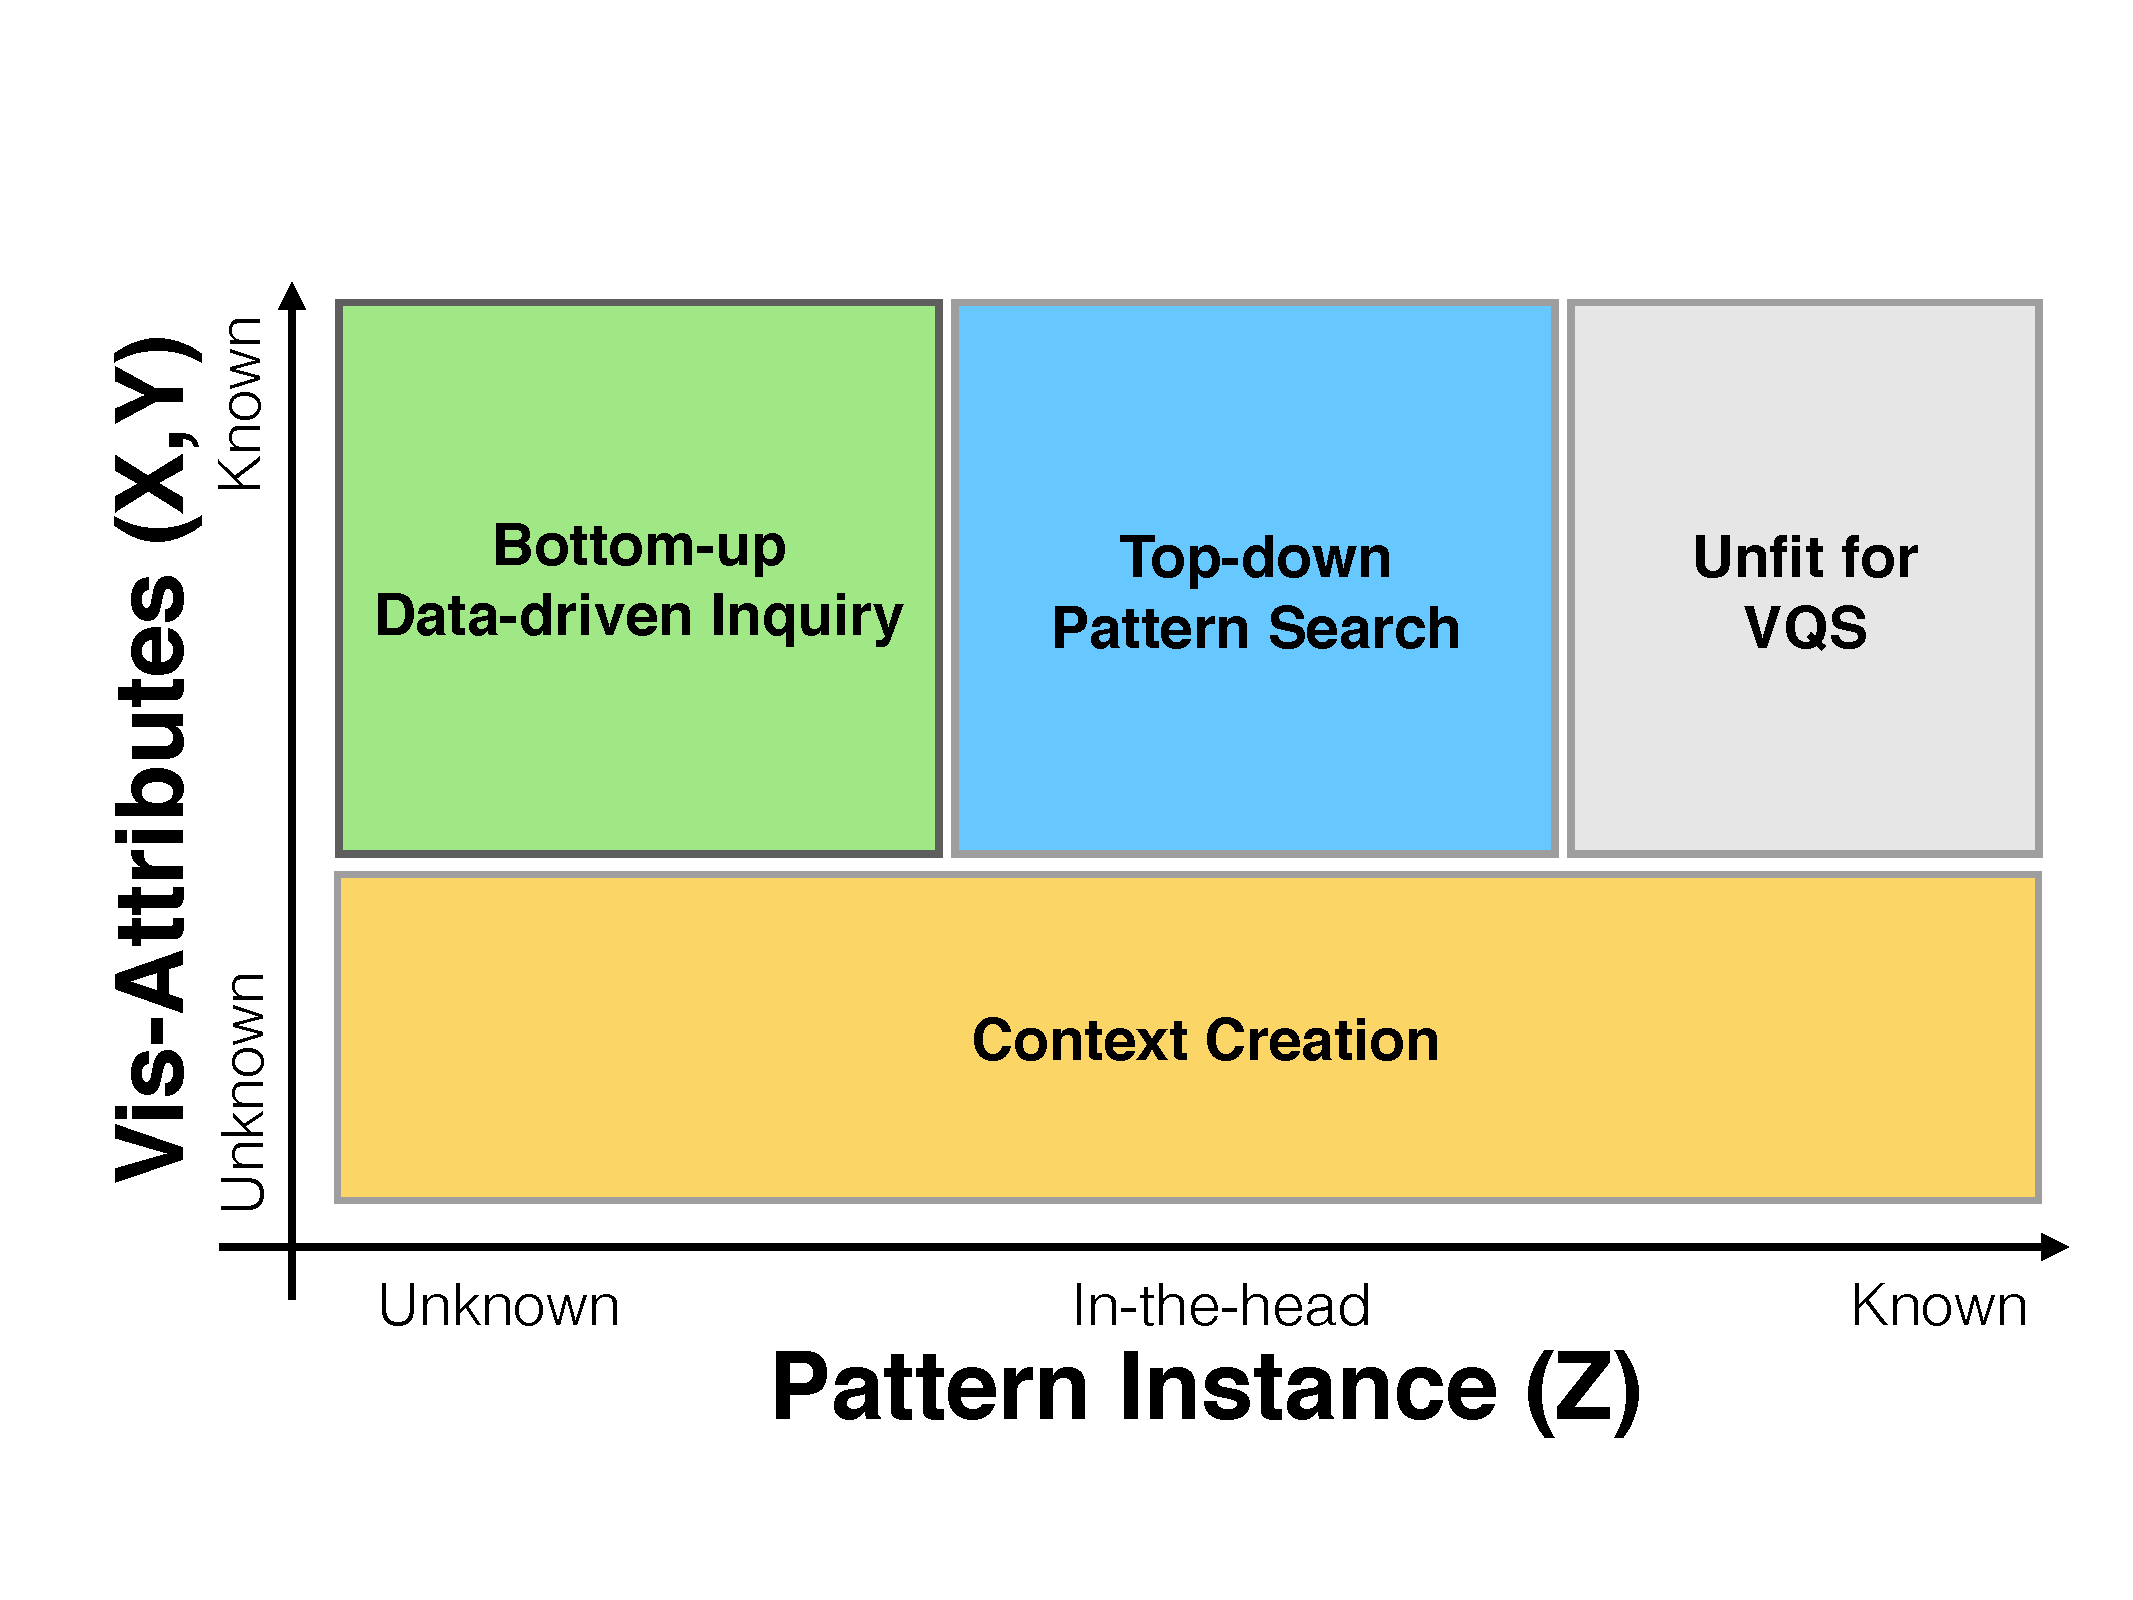
\includegraphics[width=0.5\linewidth]{figures/2dmodel.pdf}
   \caption{The problem space for VQSs is characterized by how much the analyst knows about the visualized attributes and the pattern instance. Colored areas highlight the three sensemaking processes in VQSs for addressing these characteristic problems. While prior work has focused solely on use cases in the blue region, we envision opportunities for VQSs beyond this to a larger space of use cases covered by the yellow and green regions.}
   \label{2dmodel}
   % \vspace{-10pt}
 \end{figure}
 \rchange{
  \clearpage
   \section{Evaluation Study Protocol\label{apdx:studyprotocol}}
   Here, we detail the procedures that were conducted during the evaluation study. At the beginning of the study, participants were asked a set of pre-study survey questions to collect basic information about participant's dataset, scientific questions, and existing workflows. While this information was similar to the ones collected through participatory design and contextual inquiry (Section~\ref{sec:participantdatasets}), the pre-study survey ensured that we have background information even for the ``blank-slate'' participants (who were not part of the earlier design study).
   \begin{itemize}
    \item What is your current role as a scientist? What are some examples of recent questions you have researched?
    \item Describe the workflow that you currently use to analyze and make sense of this type of data.
    \item Can you describe an interesting finding you found with your current workflow and the process you took to obtain this insight? 
   \end{itemize}
   \smallskip\par\noindent After the tutorial and overview of the system, participant's selected dataset was loaded in. Participants were asked about their familiarity with the dataset and their analytical goals for the session.
   \begin{itemize}
    \item On a scale of 1-5, how familiar are you with this dataset? How long have you been working with this dataset? If you have worked with this dataset before, is there any insight that you already know from this dataset? 
    \item What is your goal for this dataset? What are you hoping to accomplish with this dataset?
   \end{itemize}
   \smallskip\par\noindent During the main experiment, participants engaged in talk-aloud exercises as they explored their data. These two semi-structured interview questions were often posed when participants begin a new line of analytical inquiry.
   \begin{itemize}
    \item What is your current goal in this phase of the exploration? What type of insights are you hoping to obtain? 
    \item What actions are you planning to perform? How are you operationalize to achieve those goals?
   \end{itemize}
   In addition, we occasionally remind participants that they ask for help on something they want to accomplish on \zvpp, but were not sure about the sequence of interactions. They were also encouraged to use other tools in their existing workflow alongside \zvpp to perform their analysis. 
   \smallskip\par\noindent At the end of the study, we interviewed participants with a set of open-ended questions regarding their experience with \zvpp, including:
   \begin{itemize}
     \item How was \zvpp different from your existing workflow? 
     \item Can you describe how you would use \zvpp in your current workflow?
     \item On a scale of 1-10, how interested would you be in adopting this tool for your day-to-day workflow?
     \item What were some insights that you have gained from today's session?
     \item Given the insights that you have obtained from \zvpp, are there any additional analysis that you will run downstream before you publish these results? Describe these additional downstream analysis steps.
     \item What are the pros and cons for using \zvpp?
     \item Were there any queries that you were unable to address with \zvpp during today's session?
     \item What are additional features in \zvpp that would help with your scientific workflow or serve your scientific need?
   \end{itemize}
}
\clearpage
 \section{Evaluation Study Analysis Details\label{apdx:studydetails}}
 We analyzed the transcriptions of the evaluation study recordings through open-coding and
 categorized every event in the user study using the following coding labels:
 \begin{denselist}
     \item Insight (Science) \textbf{[IS]}: Insight that connected back to the science (e.g. ``This cluster resembles a repressed gene.'')
     \item Insight (Data) \textbf{[ID]}: Data-related insights (e.g. ``A bug in my data cleaning code generated this peak artifact.'')
     \item Provoke (Science) \textbf{[PS]}: Interactions or observations that provoked a scientific hypothesis to be generated.
     \item Provoke (Data) \textbf{[PD]}: Interactions or observations that provoked further data actions to continue the investigation.
     \item Confusion \textbf{[C]}: Participants were confused during this part of the analysis.
     \item Want \textbf{[W]}: Additional features that participant wants, which is not currently available on the system.
     \item External Tool \textbf{[E]}: The use of external tools outside of \zvpp to complement the analysis process.
     \item Feature Usage \textbf{[F]}: One of the features in \zvpp was used.
     \item Session Break \textbf{[BR]}: Transition to a new line of inquiry.
 \end{denselist}
 \begin{table}[h!]
 \captionsetup{font=normalsize,labelfont=normalsize}
  \centering
   \begin{tabular}{lrrrrrrrrr}
   \hline
    Domain           &   IS &   ID &   PS &   PD &   C &   W &   E &   BR &   F \\
   \hline
    astro            &    4 &   12 &   13 &   57 &   2 &  18 &  20 &   22 &  67 \\
    genetics         &    8 &   12 &    7 &   35 &   4 &  13 &   1 &   21 &  52 \\
    mat sci          &   14 &    8 &    7 &   44 &   8 &  11 &   3 &   12 &  48 \\
   \hline
   \end{tabular}
   \caption{Count summary of thematic event code across all participants of the same domain.}
   % \vspace*{-15pt}
 \end{table}
 \npar In addition, based on the usage of each feature during the user study, we categorized the features into one of the three usage types:
 \begin{denselist}
     \item Practical \textbf{[P]}: Features used in a sensible and meaningful way.
     \item Envisioned usage \textbf{[E]}: Features which could be used practically if the envisioned data was available or if they conducted downstream analysis, but was not performed due to the limited time during the user study.
     \item Not useful \textbf{[N]}: Features that are not useful or do not make sense for the participant's research question and dataset.
 \end{denselist}
 The feature usage labels for each user is summarized in Figure~\ref{feature_heatmap}. A feature is regarded as \emph{useful} if it has a \textbf{P} or \textbf{E} code label. Using the matrix from Figure~\ref{feature_heatmap}, we compute the percentage of useful features for each sensemaking process as: $\frac{\textrm{\# of useful features in process}}{\textrm{total \# of features in process} \times \textrm{total \# of users}}$.
%  \begin{figure}[h!]
%   \begin{minipage}{.5\linewidth}
%      \captionsetup{font=normalsize,labelfont=normalsize}
%      \centering
%      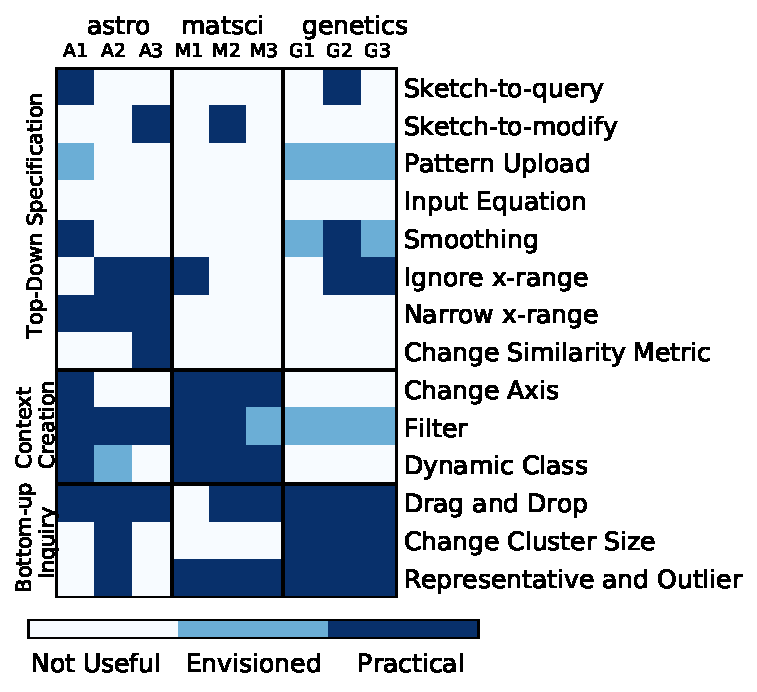
\includegraphics[width=\linewidth]{figures/PENcoding.pdf}
%      \vspace{-6pt}\caption{Heatmap of features categorized as practical usage (P), envisioned usage (E), and not useful (N). Columns are arranged in the order of subject areas and the features are arranged in the order of the three foraging acts. Participants preferred to query using bottom-up methods such as drag-and-drop over top-down approaches such as sketching or input equations. Participants found that context creation via filter constraints and dynamic class creation were powerful ways to compare between subgroups or filtered subsets.}
%      \label{feature_heatmap}
%   \end{minipage}
%   \hspace{2pt}
%   \begin{minipage}{.5\linewidth}
%     \captionsetup{font=normalsize,labelfont=normalsize}
%     \centering
%    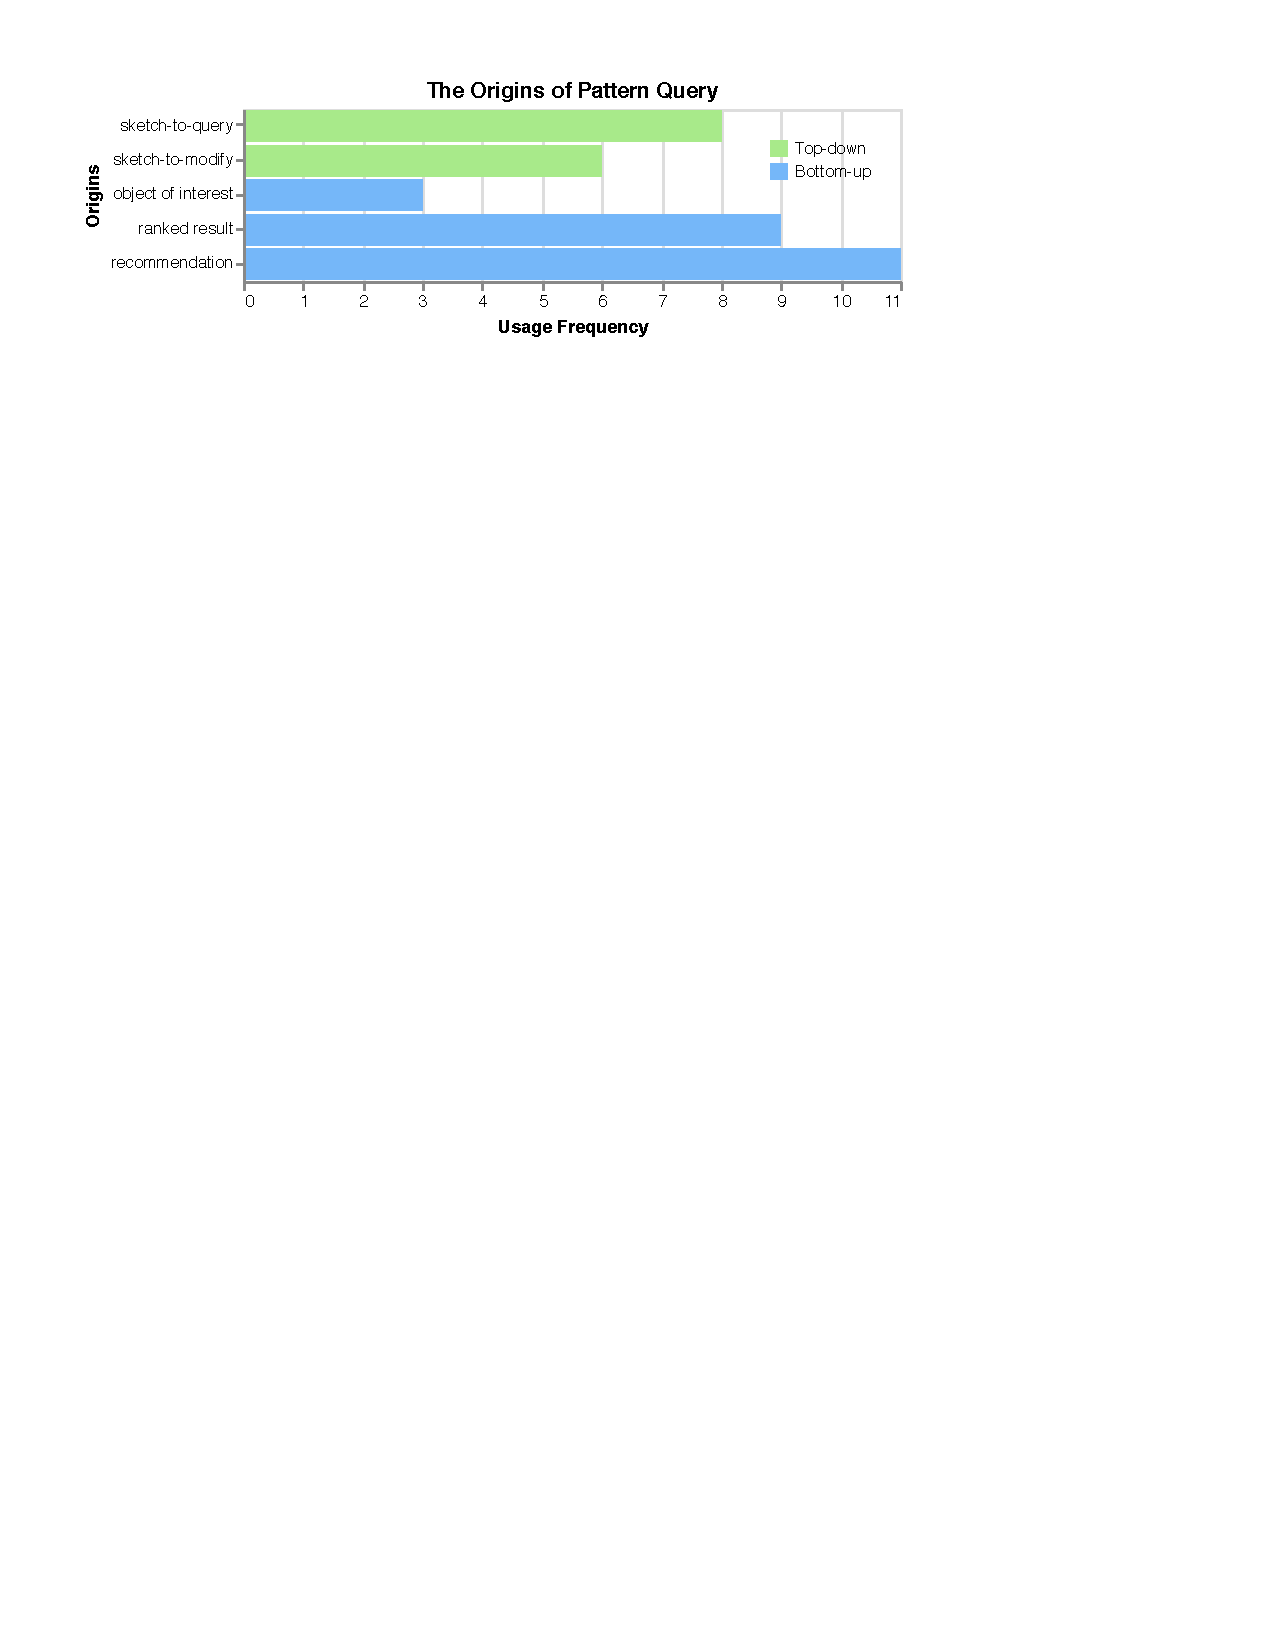
\includegraphics[width=\linewidth]{figures/the_origins_of_sketch.pdf}
%    \vspace{-5pt}
%    \caption{The number of times a pattern query originates from one of the workflows. Pattern queries are far more commonly generated via bottom-up than top-down processes.}\label{fig:origins_of_sketch}
%      \vspace*{-5pt}
%   \end{minipage}
%   \vspace*{-25pt}
% \end{figure}
 \begin{figure}[h!]
 \captionsetup{font=normalsize,labelfont=normalsize}
     \centering
     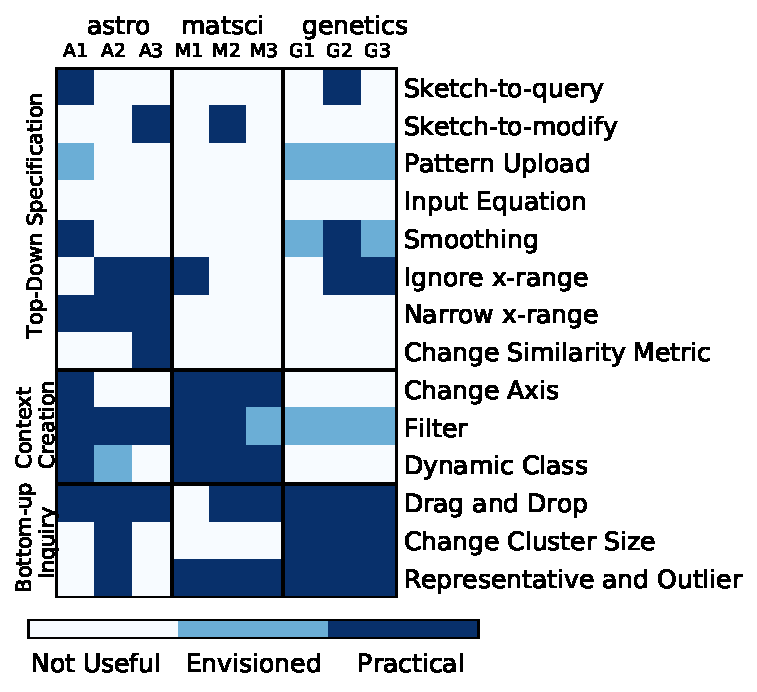
\includegraphics[width=0.45\columnwidth]{figures/PENcoding.pdf}
     \vspace{-6pt}\caption{Heatmap of features categorized as practical usage (P), envisioned usage (E), and not useful (N). Columns are arranged in the order of subject areas and the features are arranged in the order of the three foraging acts. Participants preferred to query using bottom-up methods such as drag-and-drop over top-down approaches such as sketching or input equations. Participants found that context creation via filter constraints and dynamic class creation were powerful ways to compare between subgroups or filtered subsets.}
     \label{feature_heatmap}
     % \vspace{-5pt}
 \end{figure}
 \vspace{-5pt}
 \begin{figure}[h!]
  \captionsetup{font=normalsize,labelfont=normalsize}
    \centering
   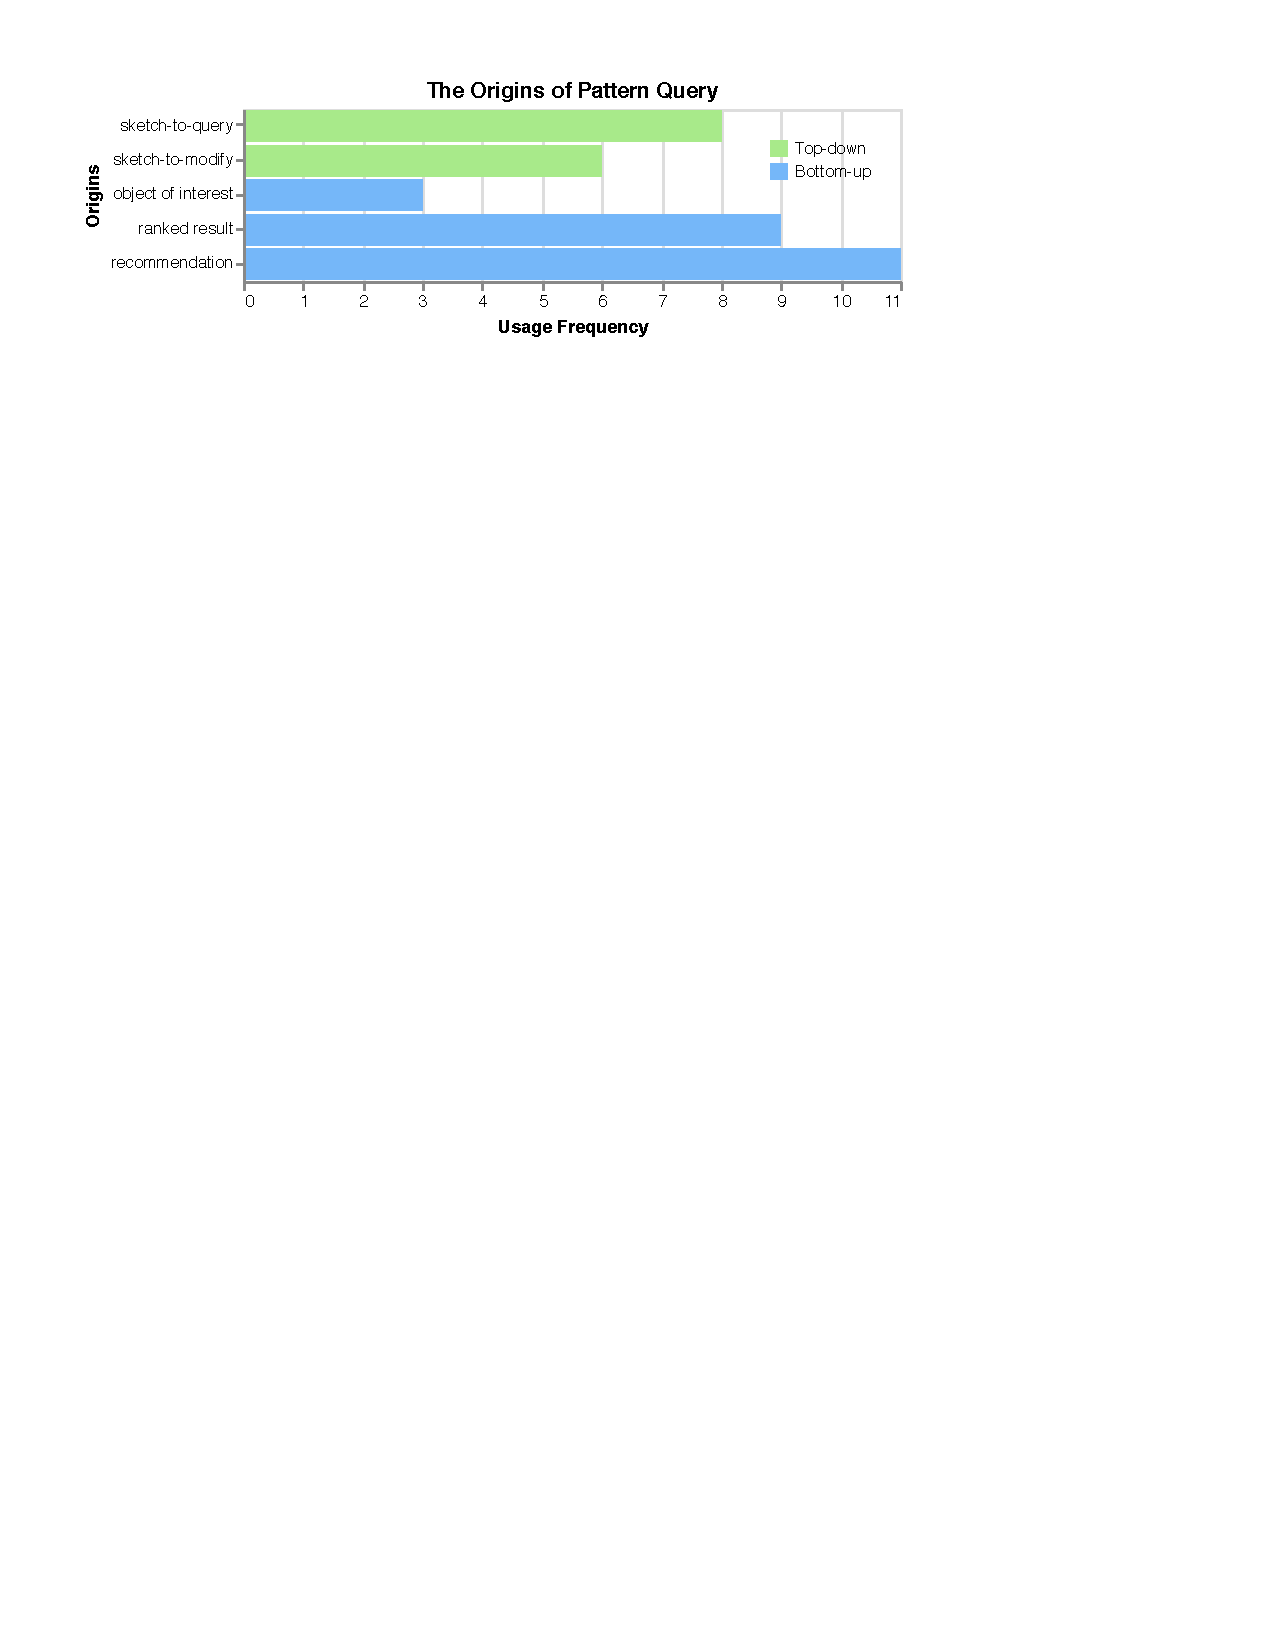
\includegraphics[width=0.55\linewidth]{figures/the_origins_of_sketch.pdf}
   \vspace{-5pt}
   \caption{The number of times a pattern query originates from one of the workflows. Pattern queries are far more commonly generated via bottom-up than top-down processes.}\label{fig:origins_of_sketch}
   % \vspace{-5pt}
 \end{figure}
 \begin{table}[h!]
  \captionsetup{font=normalsize,labelfont=normalsize}
   \centering
   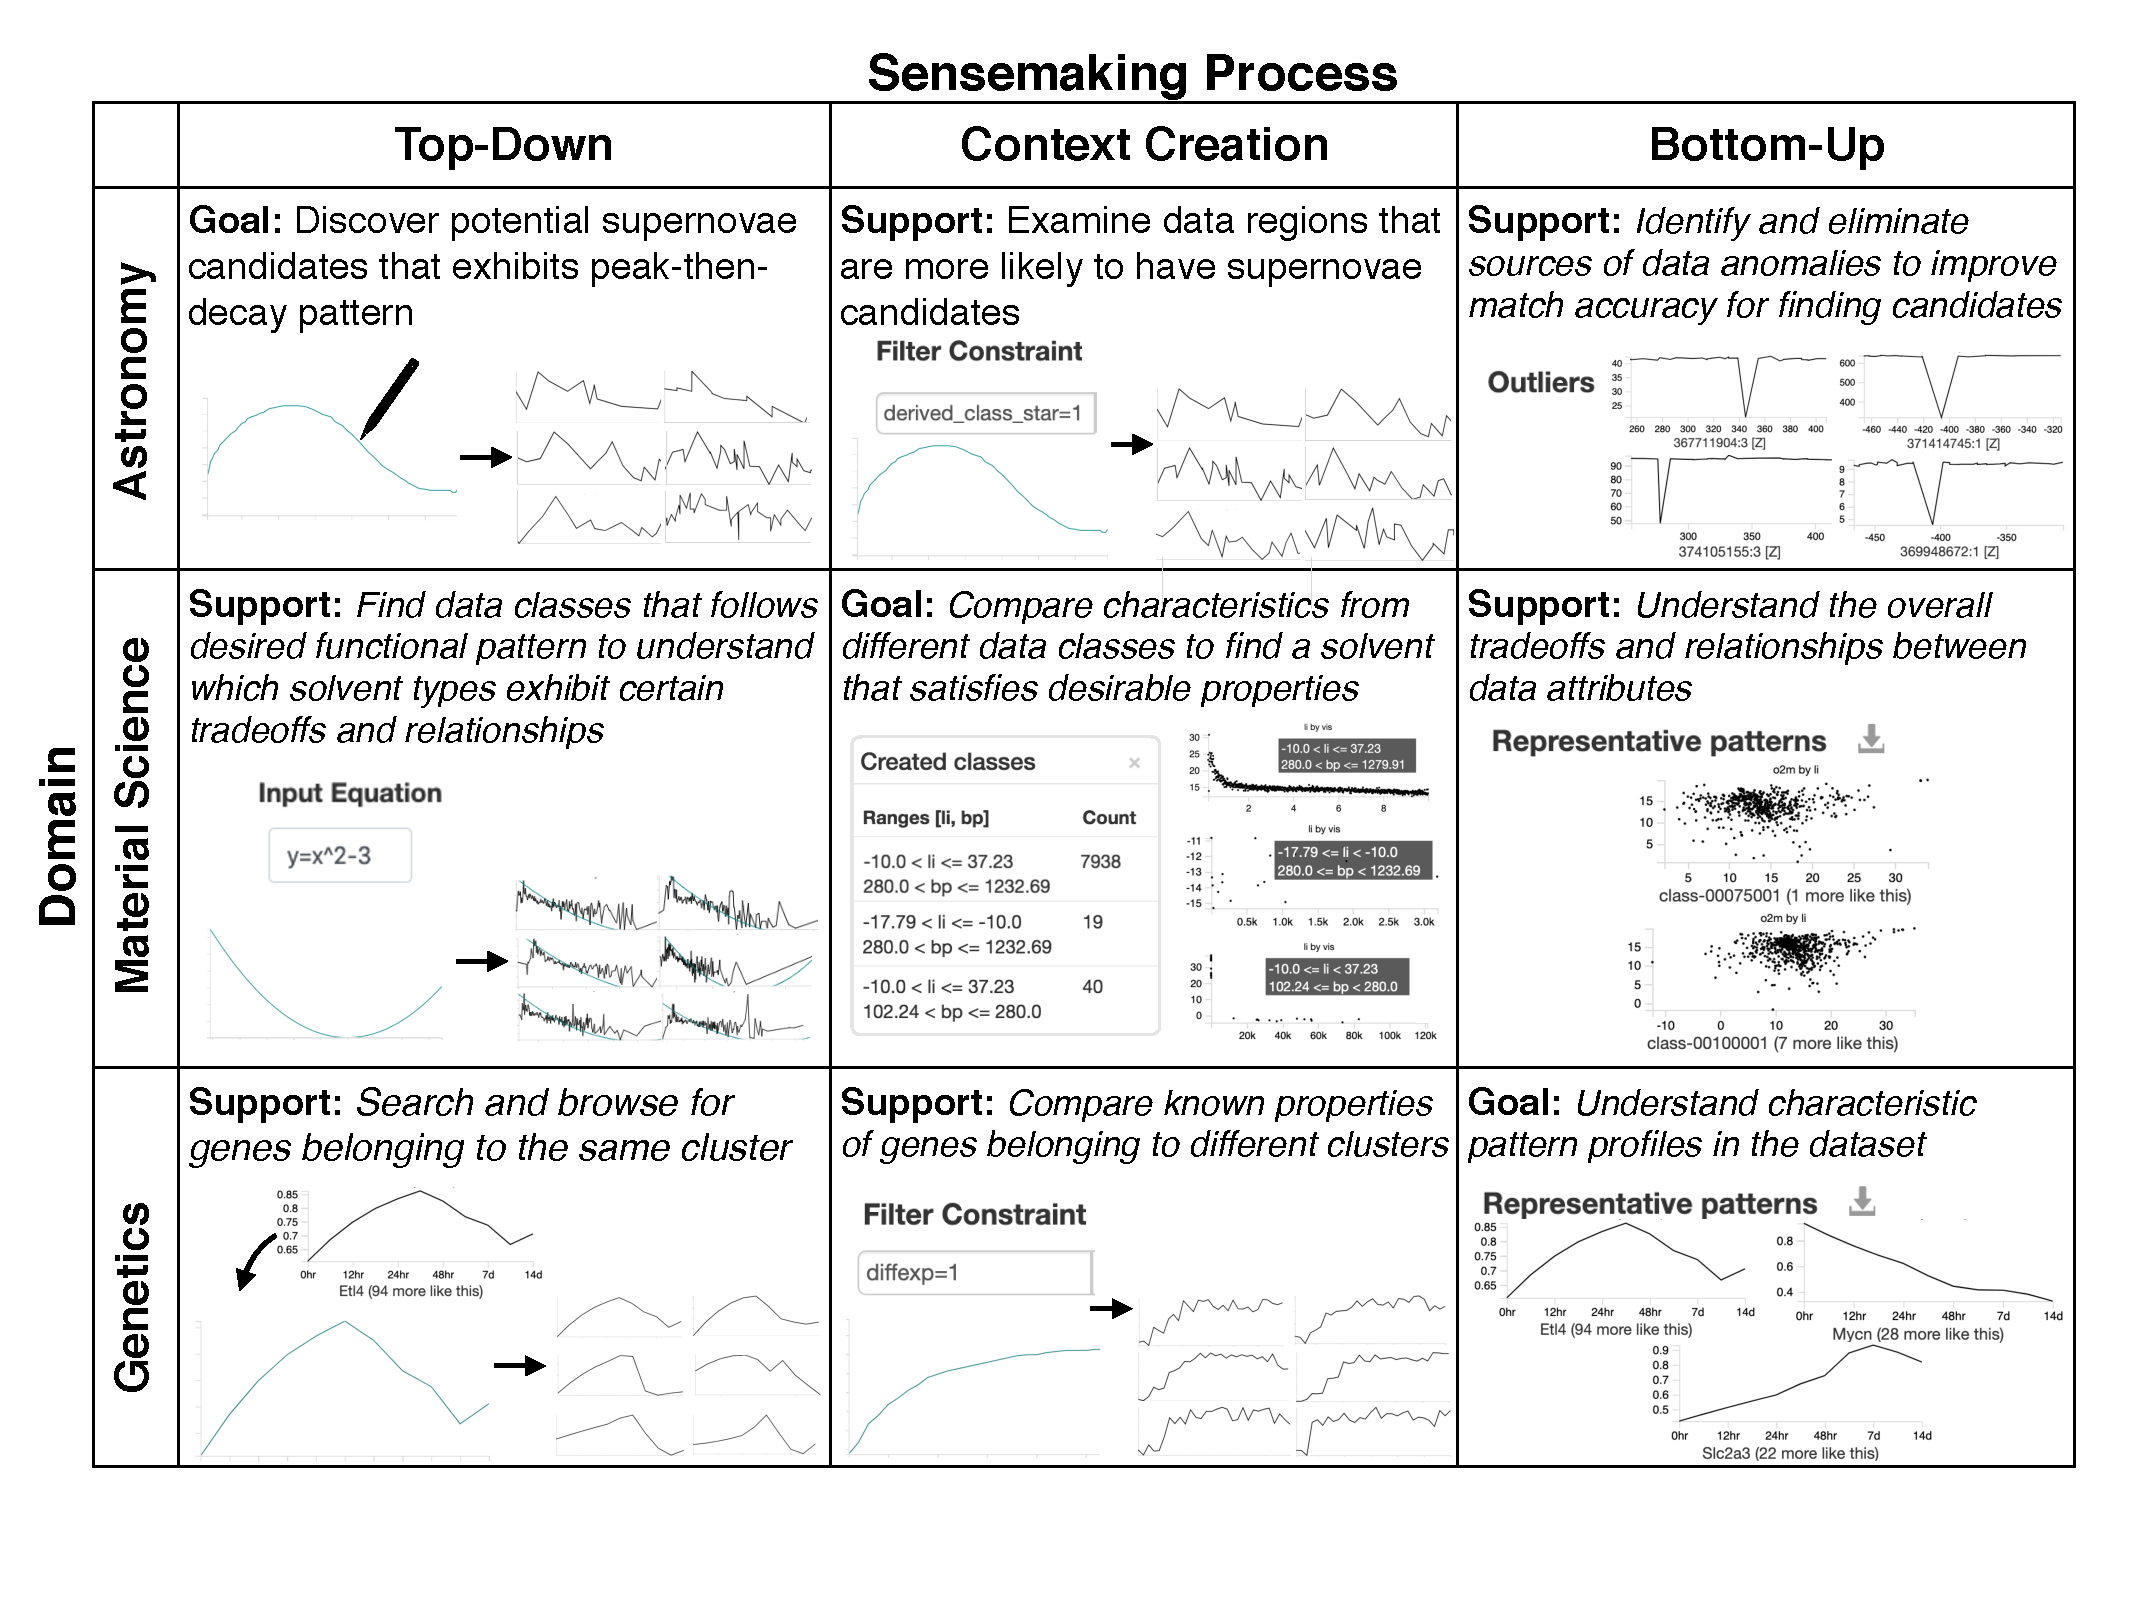
\includegraphics[width=0.85\linewidth]{figures/science_task_new.pdf}
   \caption{\rchange{Table of example usage scenarios from each domain for each sensemaking process.}\cut{Each VQS sensemaking process maps to scientific tasks and goals from each use case, from pattern search to comparing visualization collections to improving overall data understanding.} We find that our participants typically have one focused goal expressible through a single sensemaking process, but since their desired insights may not always be achievable with a single class of operation, \rchange{they make use of the two other sensemaking processes to support\cut{ (\textbf{Support})} them in accomplishing their main goal\cut{  (\textbf{Goal})}}.}%(shown with lighter background color)
   \label{science_task}
   % \vspace{-10pt}
  \cchange{
  \section{Acknowledgments}
  \begin{flushleft}
  \npar We thank Chaoran Wang, Edward Xue, and Zhiwei Zhang, who have contributed to the development of \zvpp, as well as our scientific collaborators, who provided valuable feedback during the design study. We appreciate the constructive feedback from the anonymous reviewers, which significantly improved the quality of this paper. We acknowledge support from grants IIS-1513407,IIS-1633755, IIS-1652750, and IIS-1733878 awarded by the National Science Foundation, and funds from Microsoft, 3M, Adobe, Toyota Research Institute, Google, and the Siebel Energy Institute. The content is solely the responsibility of the authors and does not necessarily represent the official views of the funding agencies and organizations.
  \end{flushleft}
  }
  %Abhishek Khetan, Matias Carrasco Kind, Vikram Pande, Pei-Chen Peng, Saurabh Sinha, and Venkat Viswanathan 
  %This paper has also benefited from discussions with Hidy Kong, Kristen Vaccaro, and Grace Yen. 
\end{table}

\end{document}

